\documentclass[a4paper]{report}

\usepackage{../mathstemplate}

\date{III семестр, осень 2023 г.}
\title{Дифференциальная геометрия. Неофициальный конспект}
\author{Лектор: Лебедева Нина Дмитриевна \\ Конспектировал Леонид Данилевич}

\begin{document}
    \shorthandoff{"}
    \maketitle
    \tableofcontents
    \newpage
    \setcounter{lection}{0}

    %Алгебраическая топология, кривые в $\R^2$ и в $\R^3$, двумерные поверхности в трёхмерном пространстве, риманова геометрия.


    \chapter{Алгебраическая топология}
    \newlection{4 сентября 2023 г.}


    \section{Применения фундаментальной группы}
    \theorem[Об инвариантности размерности]{
        $\R^n$ (при $n > 2$) не гомеоморфно никакому открытому подмножеству $U \subset \R^2$.
        \provehere{
            Рассмотрим произвольную точку $x \in U$.

            Если её удалить, то фундаментальная группа $U \sm \{x\}$ будет нетривиальной, а $\R^n \sm \{pt\}$ --- односвязно.
        }
    }
    \theorem[Об инвариантности края]{
        $\R_{\ge 0} \times \R$ не гомеоморфно никакому открытому $U \subset \R^2$.
        \provehere{
            У $\R_{\ge 0} \times \R$ можно выкинуть граничную точку, пространство останется односвязным.
        }
    }
    \definition[Ретракция топологического пространства $X \supset A$]{
        $f: X \map A$, такое, что $f\big|_A = \id$.
    }
    \theorem[Борсук]{
        Не существует ретракции двумерного диска $D^2$ на свою границу $S^1 = \partial D^2$.
        \provehere{
            От противного: пусть нашлась ретракция $f: D^2 \map S^1$. Рассмотрим композицию $S^1 \overset{\text{in}}\hookrightarrow D^2 \overset{f}{\map} S^1$.
            Композиция $\text{in} \circ f = \id_{S^1}$.

            Эта композиция индуцирует гомоморфизм фундаментальных групп $\pi_1(S^1) \overset{\text{in}_*}\Map \pi_1(D^2) \overset{f_*}{\Map} \pi_1(S^1)$, причём $\text{in}_* \circ f_* = \id_* = \id$, однако фундаментальная группа диска тривиальна.
        }
    }
    \note{
        Все предыдущие теоремы можно обобщить на случай больших размерностей, но в доказательстве будет уже не фундаментальная группа.
    }
    \theorem[Брауэр]{
        Любое непрерывное отображение $f: D^2 \map D^2$ имеет неподвижную точку.
        \provehere{
            От противного: $\exists f: D^2 \map D^2$ без неподвижных точек.

            Тогда можно построить ретракцию из диска на окружность: $x \in D^2$ отобразим в пересечение луча $f(x) \rightarrow x$ с границей $\partial D^2$.
            Назовём построенную функцию $g$.

            $g\big|_{S^1} = \id$ по определению. Для проверки непрерывности запишем $g$ формулой:
            \[g(x) = f(x) + t_{x}(x - f(x))\]
            где $t_x$ выбирается так, что $|f(x) + t_x (x - f(x))| = 1$. Таким образом, $t_x$ --- положительный (больший) корень некоего квадратного уравнения с непрерывно меняющимися коэффициентами.
        }
    }
    \theorem[Основная теорема алгебры]{
        $\forall f \in \C[x]$, $\deg f \ge 1: \exists z_0 \in \C: f(z_0) = 0$.
        \provehere[Доказательство (дама с собачкой)]{
            Запишем $f(z) = z^n + a_1 z^{n -1} + \dots + a_n$.

            Обозначим $g(z) = a_1 z^{n-1} + \dots + a_n$.
            Выберем достаточно большое $R \in \R$, такое, что $|z| \ge R \then |z^n| > |g(z)|$.

            Если $z$ пробегает все значения одного модуля $z = R \cdot e^{i t}$ по $t \in [0, 2\pi]$, то <<дама>> $z^n$ обходит большой круг $n$ раз, а <<собачка на поводке>> $g(z)$ находится внутри достаточно малого круга, что $z^n + g(z)$ не задевает нуль.
            Таким образом, $f(z) = z^n + g(z)$ пробегает некую нетривиальную петлю в $l \subset \C \sm \{0\}$ ($n$ раз оборачивающуюся вокруг нуля --- можно линейно прогомотопировать в петлю $z^n$).

            Рассмотрим гомотопию петли $\defset{t \mapsto R \cdot e^{it}}{t \in [0, 2\pi]} \subset \C$ в точку.
            Композиция $f$ с этой гомотопией создаст гомотопию петли $l$ в точку.
            Но в $\C \sm \{0\}$ петля $l$ не стягиваема, значит, применение $f$ заденет где-то $0$.
        }
    }
    \theorem[Улам-Борсук]{
        У любого $f: S^2 \map \R^2$ найдётся $x \in S^2: f(x) = f(-x)$.

        \provehere{Предположим противное. Рассмотрим функцию $g(x) \coloneqq f(x) - f(-x)$. Это нечётная функция ($g(x) = -g(-x)$), мы предполагаем, что она не обнуляется.

        Сузим $g$ на экватор сферы. $g\big|_{S^1}$ --- нечётная петля.
        \indentlemma{
            Нечётная петля имеет нечётный индекс (\emph{индекс} --- количество раз, которое петля обмоталась вокруг 0 с учётом ориентации).
        }{
            Рассмотрим $\alpha(x) = \frac{g(x)}{|g(x)|}$ --- отображение $S^1 \map S^1$, по-прежнему нечётное.

            Для определения индекса петли надо рассмотреть универсальное накрытие $\R \overset{p}\map S^1$.
            Обозначим за $\tilde{\alpha}: [0, 2\pi] \map \R$ поднятие петли $\alpha$ ($\tilde{\alpha}(0) = \tilde{\alpha}(2\pi)$).

            Без потери общности можно считать, что $\tilde{\alpha}(0) = 0$.
            Так как $\alpha$ нечётная, то $\tilde{\alpha}(\pi) = \pi(2k + 1)$ для некоего $k \in \Z$.
            Дальше из нечётности $\alpha$ получаем $\tilde{\alpha}(2\pi) = 2\pi(2k + 1)$, что и значит нечётность индекса.
        }
        Аналогично предыдущей теореме, стянем экватор $S^1$ в точку, петля стянется в точку, значит, где-то заденет $0$.}
    }


    \section{Теорема Жордана}
    \theorem[Детская версия теоремы Жордана]{
        Рассмотрим диск $D^2$, пусть $N$ и $S$ --- северный и южный полюса диска соответственно.

        Пусть $\gamma: [0, 1] \map D^2$ --- путь от $S$ до $N$, причём пусть $\gamma(0, 1) \cap S^1 = \o$.

        Тогда существуют $p, q \in D^2$, <<достаточно близкие к границе>>, такие, что $p$ и $q$ лежат в разных компонентах связности $D^2 \sm \Image(\alpha)$.
        \[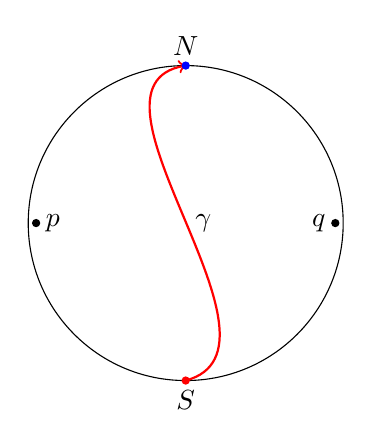
\begin{tikzpicture}
              \draw (0,0) circle (2cm);
              \node at (0,2) [above] {$N$};
              \node at (0,-2) [below] {$S$};
              \draw[red,thick,->] (0,-2) to[out=15, in=190] (0,2);
              \node at (0,0) [right]{$\gamma$};
              \fill[blue] (0,2) circle (1.5pt);
              \fill[red] (0,-2) circle (1.5pt);
              \fill (-1.9,0) circle (1.5pt) node[right] {$p$};
              \fill (1.9,0) circle (1.5pt) node[left] {$q$};
        \end{tikzpicture}\]
        \provehere{
            Выберем $p_0$ на дуге $NS$ и $q_0$ на дуге $SN$.
            Выберем внутри диска достаточно близко к $p_0$ и $q_0$, точки $p$ и $q$ соответственно (выберем так, чтобы отрезки $p p_0$ и $q q_0$ не пересекали $\Image(\gamma)$).
            Так можно сделать, так как $p_0, q_0 \notin \Image(\gamma)$, и $\Image(\gamma)$ компактно, откуда дополнение открыто.

            Теперь рассмотрим замкнутую кривую $\gamma\cdot\overset{\frown}{NS}$ (обход против часовой стрелки).
            Индекс точки $p$ относительно неё равен индексу относительно кривой $SN \cdot \overset{\frown}{NS}$ (так как можно прогомотопировать, не задевая $p$), то есть 1.
            Аналогично, индекс точки $q$ относительно этой кривой равен 0, значит, эти точки лежат в разных компонентах линейной связности $D^2 \sm \Image(\gamma)$.
        }
    }
    \intfact[Теорема Жордана]{
        Рассмотрим инъективное $S^1 \overset{\alpha}\hookrightarrow \R^2$. Тогда число компонент связности $\#(\R^2 \sm \Image(\alpha)) = 2$.
    }
    \intfact[Уточнение, теорема Шёнфлиса]{
        Эти компоненты связности гомеоморфны компонентам связности $\R^2 \sm S^1$.
    }


    \section{Ретракция. Гомотопическая эквивалентность}
    Напомним определение ретракции.
    \definition[Ретракция топологического пространства $X \supset A$]{
        $f: X \map A$, такое, что $f\big|_A = \id$.
    }

    \theorem{
        Пусть существует $r: X \map A$ --- ретракция. Тогда для отображения $\text{in}: A \map X$ индуцированный гомоморфизм фундаментальных групп $\text{in}_*$ инъективен.
        \provehere{
            Композиция $A \overset{\text{in}}\map X \overset{r}\map A$ тождественна, значит, индуцированный гомоморфизм фундаментальных групп тождественен, значит, никакие точки при $\text{in}_*$ не склеились.
        }
    }
    \definition[Деформационная ретракция $X \supset A$]{
        \emph{Гомотопия} $H: X \times [0, 1] \map X$, такая, что $\forall x \in X: H(x, 0) = x$, и $\forall a \in A: H(a, \_) = a$, причём $H(\_, 1) = A$.
    }
    \note{
        Условие $\forall a \in A: H(a, \_) = a$ можно ослаблять: некоторые определения не такие сильные --- требуют $H(a, t) \in A$ или даже только $H(a, 1) = a$.
    }
    \newlection{11 сентября 2023 г.}
    \precaution[Проблемы с доказательством теоремы Жордана]{
        Длина кривой может быть бесконечной.
        Кривая может бесконечно закручиваться, как спираль, внутрь себя (нет?)
        Легко заменить кривую на ломаную может не получиться, так как будут возникать самопересечения.
    }
    \lemma{
        Пусть $p, q$ --- концы пути $\gamma$, причём петля $\alpha$ не пересекается с носителем пути $\gamma$.
        Тогда $\textup{ind}_p(\alpha) = \textup{ind}_q(\alpha)$.
        \provehere{
            Рассмотрим гомотопию $H(x, t) = \alpha(x) - \gamma(t)$. Это непрерывная деформация $\alpha$, которая не задевает 0, значит, индексы $p$ и $q$ равны.
        }
    }
    \theorem[Шёнфлис, для ломаных]{
        Пусть $\alpha$ --- замкнутая несамопересекающаяся ломаная с вершинами $A_1, \dots, A_n$.

        Тогда плоскость бьётся на две компоненты связности, одна гомеоморфна $B_1(0)$, другая --- $\R^2\sm D_1(0)$.
        \provebullets{
            \item Докажем, что компонент связности $\R^2 \sm \Image(\alpha)$ не больше 2.
            Зафиксируем точку $p$ на границе, у неё есть окрестность, гомеоморфная $B_2$ без диаметра.

            Любую другую точку $q$ можно соединить с этой окрестностью путём, не пересекающим $\Image(\alpha)$ --- подойдём достаточно близко к кривой, дальше будем идти вдоль неё.

            Так как компонент связности $B_2$ без диаметра две, то и компонент связности $\R^2 \sm \Image(\alpha)$ не больше 2.
            \item Пусть $l$ --- прямая, не параллельная $A_i A_{i+1}$ для всех пар соседних точек (индекс берётся по модулю $n$, $A_{n+1} = A_1$).

            Пусть $N$ --- нормаль к $l$.
            Определим функцию высоты $h(p) = \angles{N, p}$.
            Все отрезки вида $A_i A_{i+1}$ не параллельны прямой $l$, их концы имеют разную высоту.

            Зафиксируем высоту $h$, рассмотрим точки пересечения $B_1, \dots, B_k$ ломаной $\alpha$ с линией уровня $h$.
            Каждой вершине $B_1, \dots, B_k$ сопоставим чётность --- $0$, если в окрестности этой вершины уровни ломаной всегда не больше (или не меньше), чем уровень данной точки.
            Иначе --- если уровень ломаной меняет знак в данной вершине --- присвоим чётность $1$.

            Каждой точке на линии уровня $h$ присвоим чётность, равную сумме (в $\Z/2\Z$) чётностей вершин левее.
            Точки с чётностями $0$ лежат снаружи ломаной, с чётностями $1$ --- внутри.

            \[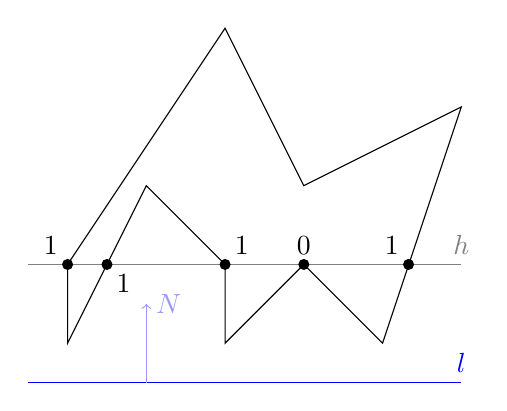
\begin{tikzpicture}
                  % Draw the polygon
                  \draw (0,0) -- (-1,1) -- (-2,-1) -- (-2,0) -- (0,3) -- (1,1) -- (3,2) -- (2,-1) -- (1,0) -- (0, -1) -- cycle;

                  % Draw the horizontal lines
                  \draw[blue] (-2.5,-1.5) -- (3,-1.5) node[above] {$l$};
                  \draw[gray] (-2.5,0) -- (3,0) node[above] {$h$};
                  \draw[blue!40,->] (-1, -1.5) -- (-1, -0.5) node[right]{$N$};

                  % Mark the points of intersection and write zeroes
                  \fill (-2,0) circle (2pt) node[above left] {$1$};
                  \fill (-1.5,0) circle (2pt) node[below right] {$1$};
                  \fill (0,0) circle (2pt) node[above right] {$1$};
                  \fill (1,0) circle (2pt) node[above] {$0$};
                  \fill (2.33,0) circle (2pt) node[above left] {$1$};

            \end{tikzpicture}\]

            По построению очевидно, что точки разных чётностей лежат в разных компонентах связности $\R^2\sm\Image(\alpha)$ (отображение $\R^2\sm\Image(\alpha) \map \{0, 1\}$, сопоставляющее точке уровень непрерывно, что проверяется ручками), а так как компонент связности не больше 2, то их ровно 2.
            \item Докажем, что множество <<нечётных точек>> гомеоморфно $B_2$.
            Для этого триангулируем их замыкание --- <<нечётные точки>>, объединённые с $\Image(\alpha)$.

            Проведя все линии уровня для $h \in \{h(A_1), \dots, h(A_n)\}$, мы получим разбиение на множество треугольников и трапеций --- трапеции несложно триангулировать.

            Склейка множества треугольников по рёбрам, как известно, даёт сферу с ручками, дырками и плёнками.

            Плёнки получиться не могут --- они неориентируемы, а $\R^2$ ориентируема.
            Но и ручки получиться не могут --- в предположении, что из плоскости получилось вырезать ручку, мы можем устроить (не деформационную) ретракцию из плоскости на окружность, что противоречит тому, что у окружности фундаментальная группа больше.
            Для этого представим ручку, как тор с дыркой --- $S^1 \times S^1$ с дыркой.
            Ретракция на окружность устроена отбрасыванием второй координаты.

            У каждой дырки есть компонента края.
            То, что дырок ровно одна, понятно из того, что край --- как-раз-таки только та (связная) ломаная $\alpha$.
        }
    }


    \section{Гомотопическая эквивалентность}
    Пусть $X, Y$ --- топологические пространства.
    \definition[Гомотопически обратные отображения]{
        Отображения $f: X \map Y, g: Y \map X$, такие, что $f \circ g \sim \id_Y$ и $g \circ f \sim \id_X$.
    }
    \definition[Гомотопически эквивалентные пространства]{
        Такие $X, Y$, что $\exists f: X \map Y, g: Y \map X$ --- гомотопически обратные отображения.

        Обозначается $X \sim Y$.
    }
    \theorem{
        Пусть $X$ --- деформационный ретракт $Y$ (достаточно самого слабого определения).
        Тогда $X \sim Y$.
        \provehere{
            Пусть $H(\_, 1) = \tau: Y \map X$ --- ретракция, $\text{in}: X \map Y$ --- включение.

            Докажем, что $\tau$ и $\text{in}$ --- гомотопически обратные.
            \bullets{
                \item $\tau \circ \text{in} = \id_X$, поэтому и гомотопически эквивалентно $X$.
                \item $\text{in} \circ \tau \sim \id_Y$ по определению деформационной ретракции.\qedhere
            }
        }
    }
    \examples[Гомотопически эквивалентные пространства]{
        \item $[0, 1] \sim [0, 1]\times[0, 1]$ --- отрезок является деформационным ретрактом квадрата.
        \item $S^1 \sim \text{лист Мёбиуса}$.
        \item Точка гомотопически эквивалентна дереву.
        \item Две разные (одномерные) восьмёрки гомотопически эквивалентны, потому что они --- ретракты третьей (двумерной) восьмёрки~(\cref{eights}).
        \pic[0.4]{eights}{Восьмёрки}
    }
    \theorem{
        Гомотопическая эквивалентность --- отношение эквивалентности.
        \provebullets{
            \item Рефлексивность: $X \sim X$, так как $\id_X$ и $\id_X$ --- гомотопически обратные.
            \item Симметричность заложена в определение.
            \item Транзитивность:
            пусть $X \underset{h}{\overset{f}\rightleftarrows} Y \underset{i}{\overset{g}\rightleftarrows} Z$, где $g \circ i, i \circ g, f \circ h$ и $h \circ f$ гомотопны постоянным отображениям соответствующего пространства.
            Таким образом, так как $i \circ g \sim \id_Y$, то \[h \circ (i \circ g) \circ f \sim h \circ f \sim \id_X\]
            Аналогично $g \circ f \circ h \circ i \sim \id_Z$.
        }
    }


    \section{Пары Борсука}
    \definition[$(X, A)$ --- пара Борсука]{
        $A \subset X$, причём $\forall Y: \forall f: X \map Y: \forall H: A \times I \map Y$: если $H(\_, 0) = f\big|_A(\_)$, то гомотопию можно продолжить: $\exists \tilde{H}:X \times I \map Y$, такая что ${\tilde{H}\big|_{A \times I} = H}$, причём $\tilde{H}(\_, 0) = f(\_)$.
    % https://q.uiver.app/#q=WzAsNSxbMCwwLCJBIl0sWzEsMSwiWCBcXHRpbWVzIEkiXSxbMSwwLCJYIl0sWzAsMSwiQSBcXHRpbWVzIEkiXSxbMiwyLCJZIl0sWzMsNCwiSCIsMCx7ImN1cnZlIjoyfV0sWzIsNCwiZiIsMCx7ImN1cnZlIjotMn1dLFswLDIsIiIsMix7InN0eWxlIjp7InRhaWwiOnsibmFtZSI6Imhvb2siLCJzaWRlIjoidG9wIn19fV0sWzEsNCwiXFx0aWxkZXtIfSIsMCx7InN0eWxlIjp7ImJvZHkiOnsibmFtZSI6ImRhc2hlZCJ9fX1dLFsyLDEsIiIsMCx7InN0eWxlIjp7InRhaWwiOnsibmFtZSI6Imhvb2siLCJzaWRlIjoiYm90dG9tIn19fV0sWzAsMywiIiwwLHsic3R5bGUiOnsidGFpbCI6eyJuYW1lIjoiaG9vayIsInNpZGUiOiJ0b3AifX19XSxbMywxLCIiLDEseyJzdHlsZSI6eyJ0YWlsIjp7Im5hbWUiOiJob29rIiwic2lkZSI6InRvcCJ9fX1dXQ==
        \[\begin{tikzcd}[ampersand replacement=\&]
              A \& X \\
              {A \times I} \& {X \times I} \\
              \&\& Y
              \arrow["H", curve={height=12pt}, from=2-1, to=3-3]
              \arrow["f", curve={height=-12pt}, from=1-2, to=3-3]
              \arrow[hook, from=1-1, to=1-2]
              \arrow["{\tilde{H}}", dashed, from=2-2, to=3-3]
              \arrow[hook', from=1-2, to=2-2]
              \arrow[hook, from=1-1, to=2-1]
              \arrow[hook, from=2-1, to=2-2]
        \end{tikzcd}\]
    }
    \newlection{18 сентября 2023 г.}
    В некотором смысле, практически все пары пространства-подпространства, которые естественно придумать, являются парой Борсука.
    Например, парами Борсука являются пары клеточного пространства и его клеточного подпространства~(\cref{cw-borsuk})
    \definition[Локально компактное пространство $X$]{$\forall x \in X: \exists U \ni x: \Cl U$ компактно.}
    \fact{\label{factor-times}
    Пусть $X \supset A$, причём $B$ локально компактно.
    Тогда $(X/A) \times B \cong (X \times B)/_\sim$, где $\forall a_1, a_2 \in A, b \in B: (a_1, b) \sim (a_2, b)$.
    \provehere{
        Равенство множеств проверить несложно, но чтобы проверить гомеоморфизм топологических пространств, надо воспользоваться локальной компактностью.

        Этот факт из общей топологии мы доказывать не будем.
    }
    }
    \note{
        $A$ --- стягиваемо $\iff \exists a \in A$: $\{a\}$ --- деформационный ретракт $A$ в самом слабом смысле.
    }
    \theorem{
        Пусть $(X, A)$ --- пара Борсука.
        Если $A$ стягиваемо, то $X \sim X/A$.
        \provehere{ Пусть $\mathcal{F}^*: A \times I \map A$ --- гомотопия, стягивающая $A$ в точку $a \in A$ (таким образом $\mathcal{F}^*\big|_{A \times \{0\}} = \id_A$ и $\mathcal{F}^*\big|_{A \times \{1\}} = a$)

            Положим в качестве $\mathcal{F}: X \times I \map X$ гомотопию, продолжающую $\mathcal{F}^*$ так, что $\mathcal{F}\big|_{X \times \{0\}} = \id_X$ (такая найдётся по определению пары Борсука).

            Так как $\forall t \in I: \mathcal{F}(A, t) \subset A$, то $(p \circ \mathcal{F})(A, t) = p(A)$ ($p(A)$ --- одноточечное множество), и $p \circ \mathcal{F}$ пропускается через фактор:
            $\exists!$ непрерывное $\tilde{\mathcal{F}}: (X\times I)/_\sim$, делающее диаграмму коммутативной.
        % https://q.uiver.app/#q=WzAsNCxbMCwwLCJYXFx0aW1lcyBJIl0sWzEsMCwiWCJdLFsxLDEsIlgvQSJdLFswLDEsIihYIFxcdGltZXMgSSkvX1xcc2ltIl0sWzAsMSwiXFxtYXRoY2Fse0Z9Il0sWzEsMiwicCJdLFswLDMsIi9fXFxzaW0iLDAseyJsYWJlbF9wb3NpdGlvbiI6MzB9XSxbMywyLCJcXHRpbGRle1xcbWF0aGNhbHtGfX0iXV0=
            \[\begin{tikzcd}[ampersand replacement=\&]
            {X\times I}
                  \& X \\
                  {(X \times I)/_\sim} \& {X/A}
                  \arrow["{\mathcal{F}}", from=1-1, to=1-2]
                  \arrow["p", from=1-2, to=2-2]
                  \arrow["{/_\sim}", from=1-1, to=2-1]
                  \arrow["{\tilde{\mathcal{F}}}", from=2-1, to=2-2]
            \end{tikzcd}\]
            Отождествляя $(X \times I)/_\sim \cong (X/A) \times I$, получаем $\tilde{\mathcal{F}}: (X / A) \times I \map X/A$, $\tilde{\mathcal{F}}(\_, 0) = \id_{X/A}$.

            Так как $\mathcal{F}(A, 1) = a$, то можно пропуститься через фактор: $\exists q: X/A \map X: q \circ p = \mathcal{F}(\_, 1)$.

            Таким образом, $q \circ p \sim \id_{X/A}$ (гомотопией является $\tilde{\mathcal{F}}$) и $p \circ q \sim \id_X$ (гомотопией является $\mathcal{F}$).
        }
    }


    \section{Клеточная пара --- пара Борсука}
    \fact{\label{about-retraction}
    Пусть $A$ замкнуто в $X$ (необязательное условие, без которого сложнее, и без которого нужна хаусдорфовость $X$).

    Рассмотрим пространство $X \times I$.
        $A \subset X$ --- пара Борсука, если $(X \times \{0\}) \cup (A \times I)$ --- ретракт $X \times I$.
        \provehere{
            Обозначим данную ретракцию за $\rho: X \times I \map (X \times \{0\} \cup A \times I)$.
            Чтобы показать, что $(X, A)$ --- пара Борсука, рассмотрим произвольное $f: X \map Y$, рассмотрим гомотопию $H: A \times I \map Y$, такую, что $H\big|_{A \times \{0\}} = f\big|_A$.

            Необходимо показать существование продолжения гомотопии $\tilde{H}: X \times I \map Y$.
            Подойдёт \[\tilde{H}: (x, t) \mapsto \all{f(\tilde{x}),&\rho(x) = (\tilde{x}, 0) \in X \times \{0\}\\ H(a, t),&\rho(x) = (a, t) \in A \times I}\]
            Непрерывность $\tilde{H}$ следует из замкнутости $A$ в $X$.
        }
    }
    \note{В обратную сторону тоже верно.}
    \note{
        $(D^n, \partial D^n) = (D^n, S^{n - 1})$ --- пара Борсука.
        \provehere{
            Цилиндр $D^n \times I$ легко можно стянуть на <<стакан>> $(D^n \times \{0\}) \cup (S^{n - 1} \times I)$.

            Пусть $y$ --- центр шара $D^n$.
            Ретракция может быть устроена следующим образом:
            \begin{align*}
                H: D^n \times I &\map (D^n \times \{0\}) \times (S^{n - 1} \times I)\\(x, t) &\mapsto \all{\left(y + (x - y) \cdot \frac{1}{d(x, y)},\frac{1}{d(x,y)}\right),&\frac{2 - t}{d(x, y)} \le 2\\\left(y + (x - y) \cdot \frac{2}{2 - t},0\right),&\frac{2 - t}{d(x, y)} \ge 2}
            \end{align*}
            Иначе говоря, берётся произведение диска $D^n \subset \R^n$ с отрезком $[0, 2]$, в качестве стакана выбирается $(D^n \times \{0\}) \cup (\partial D^n \times [0, 1])$, после чего все точки $x \in D^n \times [0, 1]$ переходят в пересечение луча $(y, 2) \rightarrow x$ и стакана.
        }
    }
    \note{
        Если $(X, A)$ и $(A, B)$ --- пары Борсука, то $(X, B)$ --- пара Борсука.
        \provehere{
            Прямо из определения.
            Пусть $f: X \map Y$, $H: B \times I \map Y$ --- отображение и гомотопия, которые надо продолжить $f\big|_{B} = H\big|_{B \times \{0\}}$.

            Так как $(A, B)$ --- пара Борсука, то $\exists H_1: A \times I \map Y$, такая, что $H_1\big|_{B \times I} = H, H_1\big|_{A \times \{0\}} = f\big|_{A}$.

            Так как $(X, A)$ --- пара Борсука, то $\exists H_2: X \times I \map Y$, такая, что $H_2\big|_{A \times I} = H_1, H_2\big|_{X \times \{0\}} = f$.
        }
    }
    \fact{
        Приклеим $n$-мерную клетку $D^n$ по её границе с помощью $f: \partial D^n \map X$.
        Назовём результат склейки $Y \coloneqq X \sqcup_f D^n$.
        Утверждается, что тогда $(Y, X)$ --- пара Борсука.
        \provehere{
            Докажем~(\cref{about-retraction}).

            $Y \times I = (X \sqcup_f D^n) \times I \underset{\text{\cref{factor-times}}}= ((X \sqcup D^n) \times I)/_\sim$, где $\sim$ порождено $(x, t) \sim (f(x), t)$ ($x \in \partial D^n, t \in I$).
            Совместив ретракцию $D^n \times I$ на стакан $D^n \times \{0\} \cup \partial D^n \times I$ и $\id_{X \times I}$, получим ретракцию
            \[\phi: (X \sqcup D^n) \times I \map X \times I \sqcup \underbrace{(D^n \times \{0\} \cup \partial D^n \times I)}_{\text{стакан}}\]
            $\phi$ пропускается через фактор: $\exists$ ретракция $\tilde{\phi}: (X \sqcup_f D^n) \times I \map (X \times I \sqcup \underbrace{D^n \times \{0\} \cup \partial D^n \times I}_{\text{стакан}})/_\sim$.
        }
    }
    Пусть $X$ --- клеточное пространство, $A \subset X$ --- замкнутое подпространство, состоящее из целого числа клеток.
    \corollary{\label{cw-borsuk}
    Клеточное пространство $X$ с клеточным подпространством $A \subset X$ --- пара Борсука.
    \provehere{
        Индукция по построению клеточного пространства --- приклеивая клетку к $X$, мы можем либо приклеить, либо не приклеить, эту клетку к $A$, в обоих случаях пара останется парой Борсука.

        Согласно транзитивности пар Борсука на выходе получится пара Борсука.
    }
    }


    \section{Гомотопическая эквивалентность и фундаментальная группа}
    Пусть $\gamma: I \map X$ путь, такой, что $p \coloneqq \gamma(0), q \coloneqq \gamma(1)$.

    Тогда $T_{\gamma}: \pi_1(X, p) \map \pi_1(X, q); [\alpha] \mapsto [\gamma\alpha \gamma^{-1}]$ --- изоморфизм фундаментальных групп.

    \theorem{
        Фундаментальные группы гомотопически эквивалентных пространств изоморфны.
        \provehere{
            Пусть $f: X \map Y, g: Y \map X$ --- отображения из определения гомотопических эквивалентностей.

            Пусть $f(x_0) = y_0$. Тогда $f$ индуцирует \emph{гомоморфизм прямого образа} $f_*: \pi_1(X, x_0) \map \pi_1(Y, y_0)$.

            Чтобы проверить, что $f_*$ --- изоморфизм групп, проверим, что это биекция. $g \circ f \sim \id_X$.
            Тогда соответствующие петли тоже получаются свободно гомотопными.

            Проверим, что петли свободно гомотопны: рассмотрим петлю $\gamma(t) \coloneqq h_t(x_0)$, где $h_t$ --- гомотопия, соединяющая $g \circ f$ и $\id_X$.
            $[\alpha] = (T_{\gamma} \circ g_* \circ f_*)([\alpha])$, откуда $T_{\gamma} \circ g_* \circ f_* = \id$.

            Воспользуемся тем, что $T_\gamma$ --- биекция ($T_{\gamma} \circ T_{\gamma^{-1}} = \id$).
            Таким образом, у $f_*$ имеется обратный слева, у $g_*$ --- обратный справа.
            Но аналогично у $f_*$ имеется обратный справа, у $g_*$ --- обратный слева, значит, это биекции.
        }
    }


    \section{Накрытия}
    \definition[Накрытие]{
        Непрерывное отображение $p: Y \map X$, такое что $\forall x \in X: \exists U \ni x$ --- правильная окрестность, такая, что $p^{-1}(U) = \bigcup\limits_{\alpha \in \Lambda}V_{\alpha}$,  причём $\forall \alpha \in \Lambda: p\big|_{V_\alpha}$ --- гомеоморфизм на $U$.
    }
    \definition[Поднятие отображения $f: Z \map X$ в накрытии]{
        Такое $\tilde{f}: Z \map Y$, что $f = p \circ \tilde{f}$.
        % https://q.uiver.app/#q=WzAsMyxbMCwxLCJaIl0sWzEsMSwiWCJdLFsxLDAsIlkiXSxbMCwxLCJmIiwyXSxbMiwxLCJwIl0sWzAsMiwiXFx0aWxkZXtmfSJdXQ==
        \[\begin{tikzcd}[ampersand replacement=\&]
              \& Y \\
              Z \& X
              \arrow["f"', from=2-1, to=2-2]
              \arrow["p", from=1-2, to=2-2]
              \arrow["{\tilde{f}}", from=2-1, to=1-2]
        \end{tikzcd}\]
    }
    Не у всякого отображения есть поднятие (например, при двулистном накрытии окружности собой нет поднятия у тождественного отображения окружности в себя).
    В прошлом семестре мы доказали, что если в $X$ есть стягиваемая петля, то её поднятие --- тоже стягиваемая петля.

    \definition[Петли, которые размыкаются при поднятии]{
        Пути $\tilde{\gamma}: [0, 1] \map X$ (являющиеся петлями, то есть $\tilde{\gamma}(0) = \tilde{\gamma}(1)$), такие, что для поднятия $\gamma$: $\gamma(0) \ne \gamma(1)$.
    }

    \fact{Для любого накрытия $p: Y \map X$: $p_*$ --- инъекция.
    \provehere{Если $\exists \alpha: p_*([\alpha]) = 0$, то $p([\alpha])$ --- стягиваемая петля, откуда $\alpha$ --- тоже, то есть $[\alpha] = e$.}}

    \definition[Группа накрытия]{
        Образ $\Image(p_*) \le \pi_1(X, x_0)$.
        Группа накрытия может зависеть от отмеченной точки $x_0$.
    }
    \definition[Локально линейно связное пространство $X$]{
        $\forall$ точки и окрестности ${x \in U \subset X}$: $\exists$ линейно связная подокрестность $V: x \in V \subset U$.
    }
    \counterexamples[Локально линейно связные и линейно связные пространства]{
        \item Конус над $\left\{\frac{1}{n}\right\}_{n = 1}^{\infty} \cup \{0\}$ линейно связен, но не локально линейно связен.
        \item Любое несвязное многообразие связно локально, но несвязно.
    }
    \newlection{25 сентября 2023 г.}
    Пусть $X, Y$ --- линейно связны, $Z$ --- линейно связное и локально линейно связное пространство.

    Рассмотрим накрытие с базой $X$ и накрывающим $Y$.
    \theorem{\label{last}
    Зафиксируем $z_0 \in Z$ и $y_0 \in p^{-1}(f(z_0))$.
    Следующие условия равносильны:
    \bullets{
        \item У $f$ найдётся единственное поднятие $\tilde{f}: Z \map Y$, такое что $\tilde{f}(z_0) = y_0$.
        \item $\Image(f_*) \subset \Image(p_*)$.
    }
    % https://q.uiver.app/#q=WzAsMyxbMCwxLCJaIl0sWzEsMSwiWCJdLFsxLDAsIlkiXSxbMCwyLCJcXHRpbGRle2Z9Il0sWzAsMSwiZiIsMl0sWzIsMSwicCJdXQ==
        \[\begin{tikzcd}[ampersand replacement=\&]
              \& Y \\
              Z \& X
              \arrow["{\tilde{f}}", from=2-1, to=1-2]
              \arrow["f"', from=2-1, to=2-2]
              \arrow["p", from=1-2, to=2-2]
        \end{tikzcd}\]
        \provetwhen{
            $f_* = p_* \circ \tilde{f}_*$.
        }{
            Пусть $\Image f_* \subset \Image p_*$.
            \bullets{
                \item
                Рассмотрим $z \in Z$, соединим с $z_0$ каким-то путём $\gamma$ ($\gamma(0) = z_0, \gamma(1) = z$).
                Путь $f \circ \gamma: [0, 1] \map X$ поднимается до какого-то пути $\alpha: [0, 1] \map Y, \alpha(0) = y_0$ единственным образом, положим $\tilde{f}(z) = \alpha(1)$.

                Понятно, что из коммутативности диаграммы нельзя выбрать $\tilde{f}(z)$ чем-нибудь другим, то есть поднятие можно определить так, и если определение корректно, то поднятие единственно.

                \item Проверим корректность определения: поднятие $z$ не зависит от пути. Пусть $z_0$ и $z$ соединяются двумя путями $\alpha$ и $\beta$.
                Тогда $f \circ (\alpha \beta^{-1})$ --- петля с началом в $x_0$. Так как $[f \circ (\alpha \beta^{-1})] \in \Image(p_*)$, то эта петля не размыкается при поднятии.

                \item Пусть $z \mapsto \tilde{f}(z)$.
                Рассмотрим любую $U \ni \tilde{f}(z)$. Для проверки непрерывности $\tilde{f}$ надо проверить, что $\exists W \ni z: \tilde{f}(W) \subset U$.

                Пусть $U'$ --- правильно накрывающая окрестность, содержащая $\tilde{f}(z)$, $p: U' \cong V$ --- гомеоморфизм.
                Заменим $U'$ на $U' \cap U$ и $V$ на $V \cap p(U)$.
                Теперь $p: U' \cong V$ — гомеоморфизм подокрестности $U$ и куска $X$.
                Берём прообраз $W_0 \coloneqq f^{-1}(V)$, это открытое множество, из коммутативности диаграммы $p \circ \tilde{f}(W_0) \subset V$.
                Выберем линейно связную подокрестность $W \subset W_0$, содержащую $z$.
                Из предыдущего равенства $p \circ \tilde{f}(W) \subset V$, но так как $V$ — правильно накрываемая окрестность, то $\tilde{f}(W)$ бьёт в дизъюнктное объединение прообразов $V$ при гомеоморфизмах, полученных из накрытия $p$.

                При этом можно убедиться, что на самом деле $\tilde{f}(W) \subset U'$: рассмотрим $w \in W$.
                Соединим $z$ и $w$ путём $\gamma$ ($\gamma(0) = z$), так, что $\Image(\gamma) \subset W$.
                Этот путь поднимается до пути $\tilde{f} \circ \gamma$ в $Y$, причём $\Image(\tilde{f} \circ \gamma) \subset p^{-1}(V)$.
                Так как $\tilde{f} \circ \gamma$ --- путь, то его концы лежат в одной компоненте связности $p^{-1}(V)$, то есть на деле в $U'$.
            }}
    }
    \ok
    \definition[Микроодносвязное или полулокально односвязное пространство $X$]{\label{good}
    $\forall x \in X: \exists U \ni x$: все петли, лежащие в $U$, стягиваемы в $X$.
    }
    Ниже считаем, что все пространства <<хорошие>>: линейно связные, локально линейно связные, микроодносвязные.

    \subsection{Морфизмы накрытий}
    Рассмотрим два накрытия с общей базой, пусть у каждого из трёх пространств отмечена некоторая точка (и морфизмы отображают отмеченную точку в отмеченную точку).
    % https://q.uiver.app/#q=WzAsMyxbMCwwLCIoWSwgeV8wKSJdLFsyLDAsIihaLCB6XzApIl0sWzEsMSwiKFgsIHhfMCkiXSxbMCwyLCJwIl0sWzEsMiwicSIsMl0sWzAsMSwiZiJdXQ==
    \[\begin{tikzcd}[ampersand replacement=\&,column sep=tiny]
    {(Y, y_0)}
          \&\& {(Z, z_0)} \\
          \& {(X, x_0)}
          \arrow["p", from=1-1, to=2-2]
          \arrow["q"', from=1-3, to=2-2]
          \arrow["f", from=1-1, to=1-3]
    \end{tikzcd}\]
    \definition[Морфизм накрытий]{
        Отображение $f$, делающее диаграмму выше коммутативной.
    }
    \note{    Требование непрерывности $f$ можно опустить, так как оно следует из доказательства~(\cref{last}).}
    \theorem{
        $\exists!$ морфизм накрытий $f \iff \Image(p_*) \subset \Image(q_*)$.
        \provehere{См.~(\cref{last}).}
    }
    \corollary{\label{cor}
    Если $p$ --- универсальное накрытие, то $\forall$ накрытия $q$: $\exists$ морфизм $f:p \map q$.
    }
    \theorem{
        Для хороших пространств универсальное накрытие существует и единственно с точностью до автоморфизма накрытий.
        \provehere{См.~(\cref{universal}).}
    }
    \definition[Автоморфизм накрытия $p: Y \map X$]{
        Такой гомеоморфизм $f$, что диаграмма коммутативна.
        % https://q.uiver.app/#q=WzAsMyxbMCwwLCIoWSwgeV8xKSJdLFsyLDAsIihZLCB5XzIpIl0sWzEsMSwiKFgsIHhfMCkiXSxbMCwyLCJwIl0sWzEsMiwicCIsMl0sWzAsMSwiZiJdXQ==
        \[\begin{tikzcd}[ampersand replacement=\&,column sep=tiny]
        {(Y, y_1)}
              \&\& {(Y, y_2)} \\
              \& {(X, x_0)}
              \arrow["p", from=1-1, to=2-2]
              \arrow["p"', from=1-3, to=2-2]
              \arrow["f", from=1-1, to=1-3]
        \end{tikzcd}\]}
    В данной категории объекты --- накрытия $p: Y \map X$ без отмеченной точки.
    \examples[Автоморфизмы]{
        \item Два накрытия $(\R, 0) \map S^1$ и $(\R, 2\pi) \map S^1$ изоморфны сдвигом \begin{align*}
                                                                                            f: (\R, 0) &\map (\R, 2\pi)\\x &\mapsto x + 2\pi
        \end{align*}
        \item В накрытии букета окружностей диаграммой свободной группы на двух образующих можно отметить любую вершину графа валентности 4.
    }
    \definition[Группа скольжения $p$]{
        Группа автоморфизмов накрытия $p$.
        Обозначается $\Aut(p)$.
    }
    \theorem{
        Если накрытие $p: Y \map X$ универсально, то $\forall y_1, y_2 \in p^{-1}(x_0): \exists!$ автоморфизм накрытия, такой, что $f: f(y_1) = y_2$.
        \provehere{ См.~(\cref{cor}).        }
    }
    \theorem{\label{regular}
    Пусть дано накрытие $p: Y \map X$. Следующие условия равносильны
    \bullets{
        \item $\forall y_1, y_2 \in p^{-1}(x_0)$ существует автоморфизм $f: f(y_1) = y_2$
        \item $\Image(p_*) \normeq \pi_1(X)$.}
    \provehere{
        Образы фундаментальных групп $\pi_1(Y, y_1)$ и $\pi_1(Y, y_2)$ при действии $p_*$ сопряжены.
        В самом деле, пусть $\gamma$ --- путь от $y_2$ до $y_1$. Пусть $\alpha$ --- петля с началом в $y_1$.
        Петле $p(\alpha)$ поставим в соответствие петлю $p(\gamma\alpha \gamma^{-1})$.

        Из теоремы о поднятии автоморфизм накрытий существует, если $\forall y_1, y_2 \in p^{-1}(x_0): \Image_{y_1}(p_*) = \Image_{y_2}(p_*)$ (выполнено включение в обе стороны), а это верно, если подгруппа нормальна.

        Если же подгруппа не нормальна, то найдётся петля, которой можно сопрячь образы так, чтобы они различались, тогда автоморфизма не будет существовать.
    }
    }
    \definition[Регулярное накрытие]{
        Накрытие, $p: Y \map X$ о котором идёт речь в ~(\cref{regular}), то есть $\Image(p_*) \normeq \pi_1(X)$.
    }
    \examples{
        \item Двулистное накрытие букета двух окружностей склейкой трёх окружностей регулярно~(\cref{two_s1s}).
        \item Трёхлистное накрытие букета двух окружностей склейкой четырёх окружностей нерегулярно (разные отмеченные точки неравноправны, нет автоморфизма, переводящего точку одного цвета в точку другого цвета)~(\cref{three_s1s})
        \begin{figure}[h!]
            \begin{minipage}{0.5\textwidth}
                \centering
                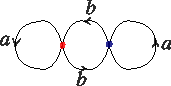
\includegraphics[width=0.4\linewidth]{two_s1s}
                \caption{\label{two_s1s}Двулистное накрытие}
            \end{minipage}
            \begin{minipage}{0.5\textwidth}
                \centering
                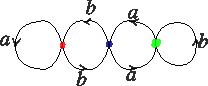
\includegraphics[width=0.4\linewidth]{three_s1s}
                \caption{\label{three_s1s}Трёхлистное накрытие}
            \end{minipage}
        \end{figure}
    }
    \theorem{\label{aut_is_pi1_factor_image}\down
    \bullets{
        \item Если накрытие $p: Y \map X$ универсально, то группа автоморфизмов накрытия $\Aut(p)$ совпадает с фундаментальной группой пространства $X$.
        \item Для произвольного регулярного накрытия $\Aut(p) = \pi_1(X)/\Image(p_*)$ (факторгруппа существует, так как $\Image(p_*)$ --- нормальная подгруппа;\ это же влечёт, что $\Image(p_*)$ не зависит от выбранной точки).
    }
    \provehere{Докажем второй пункт, первый из него следует. Зафиксируем ${y_0 \in Y: p(y_0) = x_0}$.
    Ниже определим гомоморфизм групп $\mathcal{F}: \pi_1(X) \map \Aut(p)$.

    Рассмотрим произвольную петлю $\gamma$ с концом в $x_0$.
    Её поднятие --- путь, соединяющий $y_0$ с некой точкой $y$. Так как $p(y) = x_0$, а накрытие регулярно, то найдётся автоморфизм накрытия $\tau$, такой что $\tau(y_0) = y$.
    Положим $\mathcal{F}([\gamma]) = \tau$.

    Проверим, что
    \numbers{
        \item $\mathcal{F}$ --- гомоморфизм.
        Рассмотрим петли $\gamma, \gamma'$ --- образы путей $\tilde{\gamma}$ и $\tilde{\gamma}'$, соединяющих $y_0$ с $y$ и $y'$ соответственно.
        Точкам $y$ и $y'$ соответствуют автоморфизмы $\tau$ и $\tau'$ соответственно.

        Рассмотрим путь $\tau\circ\tilde{\gamma}'$, он соединяет точку $y'$ с некой точкой, пусть это $y''$.
        Заметим, что $\mathcal{F}([\gamma] \cdot [\gamma'])$ --- это автоморфизм, переводящий $y$ в $y''$, но он же равен $\mathcal{F}([\gamma]) \cdot \mathcal{F}([\gamma']) = \tau \circ \tau'$.
        \item $\mathcal{F}$ корректно определено и сюръективно, так как каждой точке $y \in p^{-1}(x_0)$ соответствует единственный морфизм $\tau: \tau(y_0) = y$.
        \item $\Ker(\mathcal{F}) = \Image(p_*)$, так как $[\alpha] \in \Ker(\mathcal{F}) \iff$ при поднятии $\alpha$ не размыкается, а такие петли и составляют $\Image(p_*)$.\qedhere
    }
    }
    }
    \definition[Группа $G$ действует на топологическом пространстве $X$]{
        $\exists$ гомоморфизм групп $G \map \Homeo(X)$, где $\Homeo(X)$ --- группа гомеоморфизмов пространства $X$.
    }
    Назовём эквивалентными элементы $x_1, x_2 \in X$, если $\exists g \in G: g(x_1) = x_2$.
    Так как $G$ --- группа, то эквивалентными названы элементы одной орбиты, это действительно отношение эквивалентности.
    \examples{
        \item $\R \curvearrowright S^1$ --- действие поворотами.
        Все точки $S^1$ эквивалентны.
        \item Действие целочисленными сдвигами $\Z^2 \curvearrowright \R^2$ порождает тор, как факторпространство: ${\R^2/\Z^2 = T^2}$.
    }
    \newlection{2 октября 2023 г.}
    Пусть имеется действие группы на топологическом пространстве $G \curvearrowright X$.

    \definition[Действие $G\curvearrowright X$ --- накрывающее]{
        $\forall x \in X: \exists U \ni x: \{gU\}_{g \in G}$ дизъюнктны.
    }
    \examples{
        \item Универсальное накрытие $\tilde{X} \map X$. Группа автоморфизмов накрытия действует накрывающе.
    }
    \theorem{
        Если $G \curvearrowright X$ --- накрывающее, то $p: X \map X/G$ --- накрытие.
        \provehere{
            Рассмотрим $x \in X$.
            Так как действие накрывающее, то $\exists U \ni x$, такая, что $\{gU\}_{g \in G}$ дизъюнктны.
            Тогда $p(U)$ --- правильно накрываемая окрестность $p(x) \in X/G$.

            В самом деле, $p^{-1}(p(U)) = \bigsqcup\limits_{g \in G}gU$.

            Осталось проверить, что $p(U)$ открыто. Это общий факт про действие групп --- образ открытого множества открыт.
            В самом деле, $p^{-1}(p(U)) = \bigcup\limits_{g \in G}gU$, что открыто, откуда $p(U)$ открыто (по определению $V$ открыто в $X/_\sim$ $\iff p^{-1}(V)$ открыто в $X$).
        }
    }
    \corollary{
        Если $G$ действует накрывающе, и $X$ односвязно, то $G \sim \pi_1(X/G)$.
        \provehere{
            Накрытие $X \map X/G$ универсально, откуда группа автоморфизмов накрытия ($G$) совпадает с фундаментальной группой $X/G$~(\cref{aut_is_pi1_factor_image}).
        }
    }
    \theorem{
        Пусть $X$ --- хорошее пространство (существует универсальное накрытие).

        Тогда $\forall N \le \pi_1(X): \exists!$ накрытие $p: Y \map X$, такое, что $p_*(\pi_1(Y)) = N$.
        Единственность накрытия предполагается, как и следует, с точностью до изоморфизмов.
        \provehere{
            Пусть $p_0: \tilde{X} \map X$ --- универсальное накрытие.
            $G \coloneqq \pi_1(X) = \Aut(p_0)$, имеется действие $G \curvearrowright\tilde{X}, X = \tilde{X}/G$.

            Положим $Y \coloneqq \tilde{X}/N$, тогда $Y \map X$ --- накрытие с требуемой группой.
            $p_0$ пропускается через фактор.
        % https://q.uiver.app/#q=WzAsMyxbMCwwLCJcXHRpbGRle1h9Il0sWzEsMSwiWSBcXGNvbG9uZXFxIFxcdGlsZGV7WH0vTiJdLFswLDIsIlggPSBcXHRpbGRle1h9L0ciXSxbMCwyLCJwXzAiXSxbMCwxLCJwXzEiXSxbMSwyLCJcXGV4aXN0cyBwIiwwLHsic3R5bGUiOnsiYm9keSI6eyJuYW1lIjoiZGFzaGVkIn19fV1d
            \[\begin{tikzcd}[ampersand replacement=\&]
            {\tilde{X}}
                  \\
                  \& {Y \coloneqq \tilde{X}/N} \\
                  {X = \tilde{X}/G}
                  \arrow["{p_0}", from=1-1, to=3-1]
                  \arrow["{p_1}", from=1-1, to=2-2]
                  \arrow["{\exists p}", dashed, from=2-2, to=3-1]
            \end{tikzcd}\]
            Чтобы проверить, что $N = \Image(p_*)$, посмотрим, что при поднятии не размыкаются как раз петли с нужными концами.
        }
    }
    \example{
        Букет двух окружностей имеет группу $\mathcal{F}_2$. Накрытие с группой $\Z$ факторизует по одной образующей, оставляя другую. Выглядит это примерно так:
        \[\begin{tikzpicture}
              \begin{scope}[xshift=-4cm]
                  \fill (0, 0) circle (1.5pt);
                  \newcommand{\rose}[4]{ %x, y, dir, length
                      \pgfmathsetmacro{\length}{\numexpr{8 * #4}};
                      \ifnum\length>1
                      \IfStrEq{#3}{u}{\draw[<-] (#1, #2) -- ({#1}, {#2-#4})}{\rose{#1}{#2-#4/2}{d}{#4/2}};
                      \IfStrEq{#3}{d}{\draw[<-] (#1, #2) -- ({#1}, {#2+#4})}{\rose{#1}{#2+#4/2}{u}{#4/2}};
                      \IfStrEq{#3}{l}{\draw[<-] (#1, #2) -- ({#1+#4}, {#2})}{\rose{#1+#4/2}{#2}{r}{#4/2}};
                      \IfStrEq{#3}{r}{\draw[<-] (#1, #2) -- ({#1-#4}, {#2})}{\rose{#1-#4/2}{#2}{l}{#4/2}};
                      \fi
                  }
                  \rose{0}{0}{.}{3};
                  \node[above] at(0.75,0){$a$};
                  \node[above] at(-0.75,0){$a^{-1}$};
                  \node[right] at(0,0.75){$b$};
                  \node[right] at(0,-0.75){$b^{-1}$};
              \end{scope}
              \begin{scope}[xshift=3cm, yshift=2cm]
                  \fill (1.2, 0) circle (1.5pt);
                  \foreach \x in {-2.4,-1.2,0} {
                      \draw[<-] (\x, 0) -- ({\x+4}, 0);
                      \draw ({\x},{-0.5}) circle[radius=0.5];
                      \draw[->] (\x, -1) -- ({\x-0.05}, -1) node[below] {$b$};
                      \node[above] at ({\x+0.6},0) {$a^{-1}$};
                  }
                  \foreach \x in {1.2,2.4} {
                      \draw[->] ({\x-4}, 0) -- ({\x+1.2}, 0);
                      \node[above] at ({\x+0.6},0) {$a$};
                      \draw ({\x},{-0.5}) circle[radius=0.5];
                      \draw[->] (\x, -1) -- ({\x-0.05}, -1) node[below] {$b$};
                  }
                  \draw ({3.6},{-0.5}) circle[radius=0.5];
                  \draw[->] (3.6, -1) -- (3.55, -1) node[below] {$b$};
              \end{scope}
              \begin{scope}[xshift=3cm, yshift=-2cm]
                  \fill (0, 0) circle (1.5pt);
                  \draw[->] (-0.5, 0.5) -- (-0.45, 0.5);
                  \draw[->] (0.5, 0.5) -- (0.55, 0.5);
                  \draw (-0.5, 0) circle [radius=0.5];
                  \draw (0.5, 0) circle [radius=0.5];
                  \node[above] at (-0.5, 0.5) {$a$};
                  \node[above] at (0.5, 0.5) {$b$};
              \end{scope}
              \draw[->,dashed] (-1,0.5) -- (-0.2,1);
              \draw[->,dashed] (1,0.5) -- (1.5,-1);
              \draw[->,dashed] (-1,-0.5) -- (1,-1.3);
        \end{tikzpicture}\]
%        \pic[0.5]{partial_factorizing}{Накрытие букета окружностей с группой $\Z$.}
    }

    \subsection{Иерархия накрытий с общей базой}
    Пусть $\pi_1(X) \ge N_1 \ge N_2$ --- цепочка вложений групп, пусть $Y \map X$ --- универсальное накрытие.
    Тогда имеется цепочка морфизмов накрытий в обратном направлении.
    % https://q.uiver.app/#q=WzAsNCxbMCwxLCJ7WX0vTl8yID0gKFlfMiwgeV8yKSJdLFswLDIsIntZfS9OXzEgID0gKFlfMSwgeV8xKSJdLFswLDMsIlkvXFxwaV8xKFgpID0gKFgsIHhfMCkiXSxbMCwwLCJZL1xcezFcXH0gPSAoWSwgeV8wKSJdLFswLDEsInBfMiJdLFsxLDIsInBfMSJdLFszLDAsInBfMCJdXQ==
    \[\begin{tikzcd}[ampersand replacement=\&]
    {Y/\{1\} = (Y, y_0)}
          \\
          {{Y}/N_2 = (Y_2, y_2)} \\
          {{Y}/N_1  = (Y_1, y_1)} \\
          {Y/\pi_1(X) = (X, x_0)}
          \arrow["{p_2}", from=2-1, to=3-1]
          \arrow["{p_1}", from=3-1, to=4-1]
          \arrow["{p_0}", from=1-1, to=2-1]
    \end{tikzcd}\]
    Здесь, например, $p_2$ --- морфизм накрытий $p_1 \circ p_2$ и $p_1$.
    Он же является накрытием $p_2: (Y_2, y_2) \map (Y_1, y_1)$.


    \section{Фундаментальные группы клеточных пространств (CW-комплексов). Теорема Зейферта --- ван Кампена}

    \subsection{План}
    \bullets{
        \item Начинаем с одномерного остова (букета окружностей)
        \item Приклеиваем двумерные клетки, ищем соотношения
        \item Приклеиваем клетки размерности $\ge 3$, докажем, что ничего не будет меняться.
    }

    \subsection{Фундаментальная группа конечного графа}
    Пусть $X = (V, E)$ --- связный граф с $|V| = n, |E| = m$.

    Тогда $\pi_1(X)$ --- свободная группа $\mathcal{F}_{m - n + 1}$.
    \provehere{
        Выберем в графе остовное дерево $T = \left(V, \tilde{E}\right)$. $\tilde{E} = n - 1$.
        Заметим, что $(X, T)$ --- пара Борсука (клеточное пространство и подпространство).

        Стягивая $T$ в точку, получаем букет из $m - (n - 1) = m - n + 1$ окружностей.
    }

    \subsection{Теорема Зейферта --- ван Кампена}

    \subsubsection{Некоторые определения из теории групп}
    Мы будем рассматривать только конечнопорождённые конечнопредставленные группы.

    Напомним, что \emph{свободное произведение} групп $G = \angles{g_1, \dots, g_n\middle|\alpha_1, \dots, \alpha_k}$ и $H = \angles{h_1, \dots, h_m|\beta_1, \dots, \beta_l}$ --- это группа
    \[G \star H = \angles{g_1, \dots, g_n, h_1, \dots, h_m\middle|\alpha_1, \dots, \alpha_k, \beta_1, \dots, \beta_l}\]
    \examples{
        \item Свободное произведение $\Z \star \Z = \mathcal{F}_2$.
        \item <<Несвободное произведение>> $\Z \oplus \Z = \angles{a, b \middle| [a, b] = aba^{-1}b^{-1} = 1}$.
    }
    \[\text{Пусть }\begin{aligned}
                       G = &\angles{g_1, \dots, g_n\middle|\alpha_1, \dots, \alpha_k}\\ H = &\angles{h_1, \dots, h_m\middle|\beta_1, \dots, \beta_l}\\F = &\angles{f_1, \dots, f_s \middle| \gamma_1, \dots, \gamma_r}
    \end{aligned}\text{ --- группы, и зафиксированы гомоморфизмы }I: F \map G, J: F \map H.\]

    \definition[Амальгамированное произведение]{Группа
        \[G \underset{F}\star H = \angles{\arr{ccc}{g_1& \cdots& g_n\\ h_1& \cdots& h_m }\middle|\arr{ccc}{\alpha_1& \cdots& \alpha_k\\ \beta_1& \cdots& \beta_l\\ I(f_1) = J(f_1)& \cdots& I(f_s) = J(f_s)}}\]
    }

    \subsubsection{Формулировка теоремы Зейферта --- ван Кампена и доказательство для клеточных пространств}
    Пусть $X = U \cup V$, где $U, V$ --- открыты и линейно связны, $U \cap V$ линейно связно тоже.

    Выберем $x_0 \in U \cap V$, все фундаментальные группы будем рассматривать с этой отмеченной точкой.

    Имеются вложения $i: U \cap V \map U, j: U \cap V \map V$.
    Положим $I = i_*: \pi_1(U \cap V) \map \pi_1(U)$ и $J = j_*: \pi_1(U \cap V) \map \pi_1(V)$.
    \theorem[Зейферт --- ван Кампен]{
        Тогда фундаментальная группа $X$ --- это  \[\pi_1(X) = \pi_1(U) \underset{\pi_1(U \cap V)}\star \pi_1(V)\] амальгамированное произведение $\pi_1(U)$ и $\pi_1(V)$ по отношению к гомоморфизмам $I$ и $J$.
    }
    \examples[Примеры применения]{
        \item При склейке по точке никаких новых соотношений не добавляется.
        Пусть $X, Y$ --- локально односвязны.
        \[\pi_1(X \vee Y) = \pi_1(X) \star \pi_1(Y)\]
        где $\vee$ --- склейка по точке, букет.

        Для доказательства надо рассмотреть некоторую окрестность точки склейки.
        \item Например, $\pi_1(S^1 \vee S^1) = \mathcal{F}_2$.
        \item При склейке сферы из двух дисков по границе получится тривиальная группа.
        \item \textbf{23 с практики.}
        Для односвязных $A$ и $B$ и линейно связного $A \cap B$ верно, что $A \cup B$ односвязно.
        \item \textbf{24 с практики.}
        Для односвязных $A \cup B, A \cap B$ сами пространства $A, B$ тоже односвязны.
    }
    \counterexample[Важность линейной связности $U \cap V$]{
        \item При склейке двух (односвязных) отрезков по концам получится окружность с нетривиальной фундаментальной группой.
    }
    \theorem[О приклеивании двумерной клетки]{
        Пусть $Y$ --- <<хорошее>>, приклеим двумерную клетку $D^2$ по отображению $\alpha: \partial D^2 \map Y$.
        $X \coloneqq Y \sqcup_\alpha D^2$. Тогда $\pi_1(X) = \pi_1(Y)/\angles{[\alpha]}^{\pi_1(Y)}$ (где $\angles{[\alpha]}^{\pi_1(Y)}$ --- нормальное замыкание подгруппы $\angles{[\alpha]} \le \pi_1(Y)$).
        \provehere[Доказательство из теоремы Зейферта --- ван Кампена]{
            Пусть $y \in D^2$ --- центр диска.
            Рассмотрим $U = X \sm \{y\}, V = B_{\frac{1}{2}}(y)$. Тогда пересечение $U \cap V$ гомотопически эквивалентно (внутри $U \cup V$) петле $\alpha$, $\pi_1(V) = \{e\}$.
            \[\pi_1(X) = \pi_1(Y) \underset{\angles{[\alpha]}}\star \{e\} = \pi_1(Y)/\angles{[\alpha]}^{\pi_1(Y)}\]
        }
        \provehere[Другое доказательство]{
            Пусть $\alpha: S^1 \map Y, X = Y \sqcup_{\alpha} D^2, i: Y \map X, i_*: \pi_1(Y) \map \pi_1(X)$.

            Заметим, что $i_*$ --- эпиморфизм: используя лемму о свободной точке (появлялась при доказательстве того, что на $D^n$ для $n \ge 2$ всякая петля гомотопически эквивалентна несюръективной) можно гомотопией любую петлю $\beta: S^1 \map X$ привести к петле $\beta: S^1 \map Y$.
            Для этого надо рассмотреть линейное <<отталкивание>> от данной свободной точки.

            Теперь осталось проверить, что $\Ker(i_*) = \angles{[\alpha]}^{\pi_1(Y)}$.
            Очевидно включение $[\alpha] \in \Ker(i_*)$, так как ядро нормально, то $\angles{[\alpha]}^{\pi_1(Y)} \le \Ker(i_*)$.

            Рассмотрим накрытие $p_1: \tilde{Y} \map Y$ с группой $\Image((p_1)_*) = \angles{[\alpha]}^{\pi_1(Y)}$.

            Зафиксируем $w_0 \coloneqq \alpha(0) \in W$, и положим $W \coloneqq \Image(\alpha) \subset Y$, $\tilde{W} \coloneqq p_1^{-1}(W)$.
            Из регулярности накрытия: $\forall \tilde{w}_\gamma \in p_1^{-1}(w_0)$: группа накрытия с отмеченной точкой $\tilde{w}_\gamma$ --- это $\angles{[\alpha]}^{\pi_1(Y)}$.
            Так как эта группа содержит $\pi_1(W) = \angles{\alpha}$, то включение $W \hookrightarrow Y$ можно поднять, для точки $\tilde{w}_\gamma \in p_1^{-1}(w_0)$ получится $\tilde{w}_\gamma \in \tilde{W}_\gamma \cong W$.
            Иными словами, $\tilde{W}$ состоит из нескольких компонент связности $\tilde{W}_\gamma$, гомеоморфных $W$ (гомеоморфизм $p_1\big|_{W_\gamma}$).

            Приклеим к каждой такой компоненте связности $\tilde{W}_\gamma$ свой диск по отображению $\tilde{\alpha}_\gamma: \partial D^2 \map \tilde{W}_\gamma$, и назовём склейку $\tilde{X} \coloneqq \tilde{Y} \sqcup_{\{\alpha_\gamma\}} \{D^2_{\gamma}\}$.
            Пусть $\tilde{i}: \tilde{Y} \hookrightarrow \tilde{X}$ --- включение.

            Построим $p_2: \tilde{X} \map X$, такое, что $p_2\big|_{\tilde{Y}} = p_1$, и $p_2$ отображает тождественно $D^2_\gamma \map D^2$.
            Оно непрерывно, и, более того, это накрытие --- в этом несложно убедиться руками, оно очень похоже на накрытие $p_1$.

            Теперь мы готовы доказать, что $\Ker(i_*) \le \angles{[\alpha]}^{\pi_1(Y)}$.
            Рассмотрим $[\beta] \notin \angles{[\alpha]}^{\pi_1(Y)}$.
            Эту петлю можно поднять, получив разомкнутый путь $\tilde{\beta}: [0, 1] \map \tilde{Y}$.
            % https://q.uiver.app/#q=WzAsNSxbMCwxLCJbMCwgMV0iXSxbMSwxLCJZIl0sWzIsMSwiWCJdLFsxLDAsIlxcdGlsZGV7WX0iXSxbMiwwLCJcXHRpbGRle1h9Il0sWzMsNCwiXFx0aWxkZXtpfSJdLFsxLDIsImkiLDJdLFszLDEsInBfMSJdLFs0LDIsInBfMiJdLFswLDEsIlxcYmV0YSIsMl0sWzAsMywiXFx0aWxkZXtcXGJldGF9IiwwLHsic3R5bGUiOnsiYm9keSI6eyJuYW1lIjoiZGFzaGVkIn19fV1d
            \[\begin{tikzcd}[ampersand replacement=\&]
                  \& {\tilde{Y}} \& {\tilde{X}} \\
                  {[0, 1]} \& Y \& X
                  \arrow["{\tilde{i}}", from=1-2, to=1-3]
                  \arrow["i"', from=2-2, to=2-3]
                  \arrow["{p_1}", from=1-2, to=2-2]
                  \arrow["{p_2}", from=1-3, to=2-3]
                  \arrow["\beta"', from=2-1, to=2-2]
                  \arrow["{\tilde{\beta}}", dashed, from=2-1, to=1-2]
            \end{tikzcd}\]
            Из коммутативности диаграммы петля $i \circ \beta$ в $X$ при поднятии в $\tilde{X}$ размыкается точно так же.
            Значит, эта петля не стягиваема в $X$, $[\beta] \notin \Ker(i_*)$.
        }
    }
    \newlection{9 октября 2023 г.}
    Проверим, что при приклеивании клетки размерности хотя бы 3 фундаментальная группа не меняется.
    \provebullets{
        \item Рассмотрим склейку $X = D^n \sqcup_\phi Y$, и в ней петлю $\alpha: [0, 1] \map X$.
        Рассмотрим гомоморфизм вложения $\text{in}: Y \hookrightarrow X$, он индуцирует $\text{in}_*: \pi_1(Y)\map \pi_1(X)$.
        \item Применяя лемму о свободной точке, находим петле в $X$ гомотопную петлю в $Y$, значит, $\text{in}_*$ сюръективен.
        \item Проверим инъективность: $\alpha$ стягиваема в $X \then \alpha$ стягиваема в $Y$.
        $\exists$ гомотопия $H$, стягивающая $\alpha$ внутри $X$.
        Найдём точку в образе $D^n$, не покрываемую $H$.

        Представим $X = U \cup V$, где $U$ --- образ $B_{\frac12}(0)$, $V$ --- весь $X$ без образа $0$.
        $U \cap V \cong S^{n - 1} \times (0, 1)$.

        Разобьём квадрат гомотопии $[0,1]\times [0,1]$ по лемме Лебега на маленькие квадратики $K_{i,j}$, так что $H(K_{i,j}) \subset U$ или $H(K_{i,j}) \subset V$.

        Обозначим $L \coloneqq \bigcup\limits_{K_{i,j} \subset U}K_{i,j}$.
        Рассмотрим связные компоненты квадратиков из $L$, два квадратика будем считать связанными, если у них есть общая сторона.
        Тогда $L = \bigcup\limits_{i}L_i$, где $L_i$ --- объединение квадратиков, между любыми двумя из которых есть путь, в котором соседние квадратики имеют общую сторону.
        $\Image(\partial L_i) \subset U \cap V$.

        Можно представить $\partial L_i$, как образ $\alpha_i: S^1 \map [0,1]\times[0,1], \alpha_i(S^1) = \partial L_i$ (это правда только в том случае, если $L_i$ <<без дырок внутри>>;\ если есть дырки, то их можно заклеить квадратиками, присоединив их к $L_i$).
        Так как $S^{n-1}\times (0,1)$ односвязно, то петля $H \circ \alpha$ стягиваема в $U \cap V$.
        Тогда внутрь петли можно вклеить диск $D^2$.

        Таким образом, гомотопия не задевает образ центра шара, дальше <<линейным отталкиванием>> выдуваем гомотопию в $Y$.
    }

    \subsection{Фундаментальные группы основных поверхностей}
    $S_p$ --- сфера с $p$ ручками, $S_q$ --- сфера с $q$ плёнками.

    Склеим сферу с $p$ ручками, как клеточное пространство.
    \[\pi_1(S_p) = \angles{a_1, \dots, a_p, b_1, \dots, b_p\middle| a_1 b_1 a_1^{-1}b_1^{-1}\dots a_p b_p a_p^{-1}b_p^{-1}}\]
    Если посчитать абелианизацию $\pi_1(S_p)$, то есть фактор по коммутанту, то будет $\underbrace{\Z \oplus \cdots \oplus\Z}_{2p}$.
    \[\pi_1(S_q) = \angles{a_1, \dots, a_q \middle| a_1^2 \cdots a_q^2}\]
    Если посчитать абелианизацию $\pi_1(S_q)$, то есть фактор по коммутанту, то будет $\Z/2\Z \oplus \underbrace{\Z \oplus \cdots \oplus\Z}_{q - 1}$.
    \provehere{
        В качестве системы образующих $\pi_1(S_q)^{\ab}$ можно взять $a_1 \proddots a_q$ и $a_2, \dots, a_q$.
    }
    \corollary{
        Сферы с ручками и плёнками неэквивалентны друг другу.
    }
    \theorem{
        Для всякой конечнопредставленной группы $G$ $\exists$ CW-комплекс $X: \pi_1(X) = G$.
        \provehere{
            Пусть $G = \angles{a_1, \dots, a_n\middle| \alpha_1, \dots, \alpha_k}$.

            Приклеиваем клетки к букету окружностей.
        }
    }


    \section{Построение универсального накрытия}
    \theorem{\label{universal}
        Для <<хороших>> пространств существует универсальное накрытие $p: \tilde{X} \map X$.
        \provehere{
            Пусть $X$ --- <<хорошее>>, то есть линейно связное, локально линейно связное, полулокально односвязное~(\cref{good}).
            \bullets{
                \item Построим $\tilde{X}$, как множество.
                Зафиксируем $x_0 \in X$.
                Пусть $PX = \defset{\alpha: [0, 1] \map X}{\alpha(0) = x_0}$.
                $\tilde{X} = PX/_\sim$ --- пути, профакторизованные по гомотопности, связанной на концах.
                \item Определим $p: \tilde{X} \map X, p([\alpha]) = \alpha(1)$.
                \item Введём на $\tilde{X}$ топологию. Назовём $U \subset X$ хорошим, если оно открыто, линейно связно, любая петля в $U$ стягиваема в $X$.

                Введём базу топологии для $\tilde{X}$. Зафиксируем хорошее $U \subset X$.

                Пусть $\alpha \in PX, \alpha(1) \in U$; обозначим через $U_{\alpha} \coloneqq \defset{[\alpha s]}{s\text{ --- путь в $U$ с началом в $\alpha(1)$}} \subset \tilde{X}$.
                \indentlemma{
                    Если $[\beta] \in U_{\alpha}$, то $U_{\beta} = U_{\alpha}$.
                }{
                    Пусть $\beta \sim \alpha s$.
                    Проверим включение в обе стороны.
                    $\forall [\gamma] \in U_{\alpha}, \gamma \sim \alpha s_1$, откуда $\gamma \sim \alpha s \cdot s^{-1} s_1$.
                    Аналогично $U_{\beta} \subset U_{\alpha}$.
                }

                Проверим, что $\defset{U_{\alpha}}{\alpha \in PX,U\text{ --- хорошее}}$ образуют базу топологии, то есть $U_\alpha \cap V_\beta = \bigcup W_{\gamma}$ для неких $W_\gamma$.
                $\alpha(1) \in U, \beta(1) \in V$.
                Пусть некий $[\gamma] \in U_{\alpha} \cap V_{\beta}$, в частности, $\gamma(1) \in U \cap V$.
                Надо проверить, что $[\gamma]$ содержится в $U \cap V$ вместе с некой окрестностью.

                В качестве $W$ выберем хорошую окрестность $\gamma(1)$, содержащуюся в $U \cap V$ (достаточно выбрать линейно связную компоненту $U \cap V$).
                Достаточно проверить, что $W_{\gamma} \subset U_{\alpha}, V_{\beta}$, это правда.
                \item Докажем, что $p$ --- накрытие.
                Пусть $U \subset X$ --- хорошее. $p^{-1}(U) = \bigsqcup\limits U_{\alpha}$.
                В самом деле, если $U_{\alpha} \cap U_{\beta}$ непусто, то $U_{\alpha} = U_{\beta}$.

                $p^{-1}(U)$ --- классы путей с концами в $U$. $p$ непрерывно и открыто (проверяем на базе).

                Проверим, что $p\big|_{U_\alpha}$ --- биекция.
                То, что это сюръекция --- очевидно, почему $p$ --- инъекция?

                Рассмотрим $[\gamma_1], [\gamma_2] \in U_{\alpha}$, предположим, что $p([\gamma_1]) = p([\gamma_2])$.
                Тогда $\gamma_1(1) = \gamma_2(1)$, и каждый из них представим в виде $\alpha \cdot s$.
                Тогда пути $s_1$ и $s_2$ гомотопны, потому что окрестность хорошая, и $s_1 s_2^{-1}$ --- петля.
                \item Докажем, что $\tilde{X}$ линейно связно.
                Для этого посмотрим на поднятие путей из $X$ в $\tilde{X}$.
                Зафиксируем в соответствии с $x_0 \in X$ постоянный путь $\tilde{x}_0 = [\const_{x_0}] \eqqcolon \alpha_0 \in \tilde{X}$.

                Рассмотрим $\alpha \in PX$.
                У него имеется поднятие $\tilde{\alpha}: [0, 1]\map\tilde{X}$, такое, что $\tilde{\alpha}(0) = \alpha_0$.

                Заметим, что $\tilde{\alpha}(t) \sim \alpha\big|_{[0, t]}$.
                Таким образом, $\tilde{X}$ линейно связно: $\tilde{\alpha}$ соединяет $\alpha_0$ и $[\alpha]$.
                \item Проверим односвязность $\tilde{X}$.

                Пусть $\tilde{\alpha}: [0,1] \map \tilde{X}$ --- петля. Спроецируем её: $\alpha \coloneqq p \circ \tilde{\alpha}$.

                Так как $\tilde{\alpha}$ --- петля, то $[\alpha_0] = \tilde{\alpha}(0) = \tilde{\alpha}(1) = [\alpha]$, то есть $\alpha$ --- стягиваема.
                Но $\tilde{\alpha}$ --- поднятие $\alpha$, а поднятие стягиваемой петли стягиваемо.\qedhere
            }
        }
    }
    Кстати, мы уже доказали, что если накрытие существует, то оно единственно.


    \chapter{Дифференциальная геометрия}
    \newlection{16 октября 2023 г.}


    \section{Дифференциальная геометрия кривых}
    \definition[Гладкая функция $f$]{Бесконечно дифференцируемая функция ${f \in C^{\infty}(\R^n \map \R^m)}$.}

    Пусть $(X, d)$ --- метрическое пространство.
    \definition[Путь (кривая)]{
        Непрерывное $\gamma: I \map X$, где $I$ --- выпуклое подмножество прямой.
        Чаще всего рассматривают $I = [a, b]$.
    }
    \definition[Гладкая кривая]{
        Гладкое отображение $I \map \R^n$ (все координатные отображения гладкие).
    }
    \precaution{
        Необязательно гладкое отображение выглядит гладким.
        График $|y| = x^{\nicefrac{3}{2}}$ представим, как гладкая кривая $\gamma(t) = (t^2, t^3)$.
        \[\begin{tikzpicture}
              \draw[->] (-3,0) -- (3,0) node[right] {$x$};
              \draw[->] (0,-3) -- (0,3) node[above] {$y$};
              \draw[scale=1,domain=-1.6:1.6,blue] plot ({\x*\x},{0.5*\x*\x*\x});
        \end{tikzpicture}\]
    }
    \definition[Регулярная кривая]{
        Гладкая кривая $\gamma$, такая, что $\forall t: |\gamma'(t)| \ne 0$.
    }
    Пусть $\gamma_1, \gamma$ --- две кривые.
    \definition[$\gamma_1$ --- перепараметризация $\gamma$]{
        $\exists$ строго возрастающее $\phi$: $\gamma_1 = \gamma \circ \phi$.
    }
    Для гладких кривых вводят \emph{гладкую перепараметризацию} $\phi \in C^{\infty}$, $\phi' > 0$.
    \definition[Кривые $\gamma_1, \gamma_2$ эквивалентны]{
        Существует перепараметризация $\phi$.
        Пишут $\gamma_1 \sim \gamma_2$
    }
    \fact{
        Эквивалентность кривых --- отношение эквивалентности.
        Аналогичный факт верен для эквивалентности гладких перепараметризаций гладких кривых.
    }
    \definition[Разбиение отрезка $\lbrack a, b\rbrack$]{
        Разбиение $a = t_0 \le \cdots \le t_k = b$.
    }
    \definition[Длина кривой $\gamma: \lbrack a, b\rbrack \map X$]{
        $L(\gamma) \bydef \sup\limits_{a = t_0 \le \cdots \le t_k = b} \sum\limits_{i = 0}^{k-1}d(\gamma(t_i), \gamma(t_{i + 1}))$
    }
    \note{
        Согласно неравенству треугольника, при измельчении разбиения $\sum\limits_{i = 0}^{k-1}d(\gamma(t_i), \gamma(t_{i + 1}))$ возрастает.
    }
    \definition[Кривая спрямляемая]{$L(\gamma) < \infty$}
    \example{
        Неспрямляемую кривую придумать несложно.
        Например, соединим ломаной соседние точки в последовательности $(\alpha_n, (-1)^n\beta_n)$, где $\alpha_n, \beta_n$ --- убывающие, стремящиеся к нулю, последовательности, причём $\sum\limits_{n \ge 0}\beta_n = \infty$.
    }
    \proposal{
        $\gamma_1 \sim \gamma_2 \then L(\gamma_1) = L(\gamma_2)$.
    }
    \statement{
        Если кривая $\gamma$ гладкая, то $L(\gamma) = \int\limits_{a}^{b}|\gamma'(t)|\d t$.\provehere{
            Докажем неравенство в обе стороны.
            \bullets{
                \item $\int\limits_{a}^{b}|\gamma'(t)|\d t \le L(\gamma)$.

                $\gamma'$ равномерно непрерывна. Таким образом, $\forall \eps > 0: \exists \delta > 0: |t_1 - t_2| \le \delta \then |\gamma'(t_1) - \gamma'(t_2)| < \eps$.
                Разобьём отрезок на $\ceilfrac{b - a}{\delta}$ частей равной длины (каждая часть имеет длины не больше $\delta$) точками $a = t_0 \le \cdots \le t_k = b$.

                Обозначим $\phi_i(t) \coloneqq \gamma'(t_i) - \gamma'(t)$. Из равномерной непрерывности $|\phi_i(t)| < \eps$ на $[t_i, t_{i + 1}]$.
                \multline{
                    \int\limits_{t_i}^{t_{i+1}}(|\gamma'(t)| - \eps)\d t \le \int\limits_{t_i}^{t_{i+1}}|\gamma'(t_i)|\d t = \abs{\int\limits_{t_i}^{t_{i+1}}\gamma'(t_i)\d t} = \abs{\int\limits_{t_i}^{t_{i+1}}(\gamma'(t) + \phi_i(t))\d t} \le \\
                    \le \abs{\int\limits_{t_i}^{t_{i+1}}\gamma'(t)\d t} + \abs{\int\limits_{t_i}^{t_{i+1}}\phi_i(t)\d t} \le \abs{\gamma(t_{i+1})-\gamma(t_i)} + \eps|t_{i+1}-t_i|
                }
                Получаем $\int\limits_{a}^{b}|\gamma'(t)|\d t - 2\eps|b -a| \le L(\gamma)$. Устремим $\eps \to 0$.
                \item $L(\gamma) \le \int\limits_{a}^{b}|\gamma'(t)|\d t$.

                Зафиксируем $a = t_0 \le \cdots \le t_k = b$.
                Оценим $|\gamma(t_{i + 1}) - \gamma(t_i)| = \abs{\int\limits_{t_i}^{t_{i + 1}}\gamma'(t)\d t} \le \int\limits_{t_i}^{t_{i + 1}}\abs{\gamma'(t)}\d t$.\qedhere
            }
        }
    }
    \corollary{
        $\int\limits_{a}^{b}|\gamma'(t)| \d t$ не зависит от перепараметризации.
    }
    \theorem{
        Отрезки в $\R^n$ кратчайшие.
        Иными словами, $\forall r, s \in \R^n$ отрезок \begin{align*}
                                                           \alpha: [0, 1] &\map \R^n\\t &\mapsto r + t(s - r)
        \end{align*}
        имеет наименьшую длину среди всех кривых (необязательно гладких), соединяющих $r$ и $s$.
        \provehere{
            Рассмотрим путь $\gamma$, соединяющий $r$ и $s$.
            Рассмотрим разбиение $a = t_0 \le t_1 = b$.
            По определению $L(\gamma) \ge \abs{\gamma(b) - \gamma(a)}$.
        }
    }
    \theorem{
        Кратчайшие пути на сфере $S^2$ --- дуги больших кругов.
        \provehere{
            Покажем, что $\forall \gamma: [a, b] \map S^2: L(\gamma) \ge \angle(\gamma(a), \gamma(b))$.
            Выберем $\eps > 0$, из равномерной непрерывности $\gamma$ найдётся $\delta > 0: |t_1 - t_2| \le \delta \then \abs{\gamma(t_1)  - \gamma(t_2)} < \eps$.

            Рассмотрим разбиение $a = t_0 \le \cdots \le t_k = b$, такое, что $\abs{t_{i + 1} - t_i} \le \eps$.
            \[L(\gamma) \ge \sum\limits_{i = 0}^{k - 1}|\gamma(t_i) - \gamma(t_{i + 1})| \ge \sum\limits_{i = 0}^{k - 1}\angle(\gamma(t_i), \gamma(t_{i + 1}))\cdot\frac{\eps}{2\arcsin\left(\nicefrac{\eps}{2}\right)} \ge \angle(\gamma(a), \gamma(b)) \cdot \frac{\eps}{2\arcsin\left(\nicefrac{\eps}{2}\right)}\]
            Устремляем $\eps \to 0$.
        }
    }

    \subsection{Параметризация кривой длиной дуги}
    Пусть $\gamma: [a, b] \map X$, где $(X, d)$ --- метрическое пространство.
    \definition[Натуральная параметризация]{
        Такая параметризация $\gamma$, что $\forall t_1, t_2 \in [a, b]$: $L\left(\gamma\big|_{[t_1, t_2]}\right) = t_1 - t_2$.
    }
    \statement{
        Гладкая кривая параметризована натурально $\iff \abs{\gamma'} \equiv 1$.
        \provetwhen{
            Если $\exists t_0: \gamma'(t_0) = 1 + \delta$, то $\exists \eps > 0: |t - t_0| < \eps \then |\gamma'(t)| - |\gamma'(t_0)| \le \frac{\delta}{2}$.
            Тогда так как длина --- интеграл модуля производной, то в $\eps$-окрестности $t_0$ не выполняется определение натуральной параметризации.
        }{
            Длина --- интеграл модуля производной.
        }
    }
    \theorem{
        Для любой регулярной кривой существует натуральная параметризация.
        Эта параметризация единственна с точностью до сдвига на константу: если $\gamma: [a, b] \map X$ --- натуральная параметризация, то натуральной параметризацией является ещё и
        \begin{align*}
            \tilde{\gamma}: [a + c, b + c] &\map X\\t + c &\mapsto \gamma(t)
        \end{align*}
        \provehere{
            Пусть $\gamma: [a, b] \map \R^n$.

            Предъявим натуральную параметризацию: $s: [a, b] \map [0, L(\gamma)] \qquad s(t) = L\left(\gamma\big|_{[a, t]}\right) = \int\limits_{a}^{t}|\gamma'(t)|\d t$.
            \[s'(t) = |\gamma'(t)| > 0,\text{ поэтому $s$ --- валидная перепараметризация.}\]
            Положим $\gamma_1 = \gamma \circ s^{-1}$.
            \[\gamma_1' = (\gamma \circ (s^{-1}))' = \gamma' \cdot \frac{1}{s'} \quad \then \quad |\gamma_1'| = \frac{|\gamma'|}{|\gamma'|} = 1\]
            Если же есть две перепараметризации $\gamma_1 = \gamma_2 \circ\phi$, то $|\gamma_1'| = |\gamma_2'| \cdot |\phi'|$, откуда $|\phi'| = 1$.
            Используя $\phi' > 0$, получаем, что $\phi$ --- сдвиг на константу.
        }
    }
    \statement[Правило Лейбница]{
        Пусть $A: I \map \R^n, B: I \map \R^m$; пусть $*: \R^n \times \R^m \map \R^k$ --- билинейно.
        Тогда у отображения $A * B: I \map \R^k$ производная считается по правилу
        \[(A * B)' = A' * B + A * B'\]
        \provehere{\multline{\lim\limits_{t \to t_0}(A(t)*B(t) - A(t_0)*B(t_0)) = \lim\limits_{t \to t_0}A(t)*(B(t) - B(t_0)) +\\+ \lim\limits_{t \to t_0}(A(t) - A(t_0))*B(t_0) = A(t_0)B'(t_0) + A'(t)B(t_0)}}
    }
    \examples{
        \item В качестве $*$ может выступать скалярное произведение, векторное произведение, умножение вектора на число (и вообще умножение матриц)\ldots
    }


    \section{Кривизна плоской кривой, базис Френе}
    Далее везде считаем, что кривая $\gamma: [a, b] \map \R^2$ параметризована натурально, то есть $|\gamma'| = 1$.
    Будем обозначать $v = \overrightarrow{v} = \gamma'$ --- вектор скорости.
    \definition[Базис Френе]{
        Пара $(v, n)$, такая, что $v \perp n$, причём $(v, n)$ --- правый ортонормированный базис.
        Данный вектор $n$ --- \emph{нормаль к плоской кривой}.
    }
    Так как $\angles{v, v} = 1$, то $\angles{v', v} = 0$, откуда $v' \perp v$ и $\exists! \kappa \in \R: v' = \kappa n$.
    \definition[Кривизна плоской кривой]{
        Данное число $\kappa$ (на самом деле это функция $\R \map \R$, причём гладкая: $\kappa = \angles{v', n}$).
    }
    \precaution{
        $\kappa$ --- кривизна двумерной кривой (кривизна со знаком).

        Если же работать в более, чем двумерном пространстве, то у кривизны не будет знака. Там
        \[v \coloneqq \gamma' \quad N = \frac{\gamma''}{|\gamma''|}\]
        Кривизна без знака обозначается $k \coloneqq |\gamma''|$.
    }

    \subsection{Формулы Френе}
    \bullets{
        \item По определению кривизны $v' = \kappa n$
        \item $\angles{n, v} = 0$, откуда $\angles{n', v} + \angles{n, v'} = 0$, откуда $n' = -\kappa v$.
    }
    \newlection{23 октября 2023 г.}

    \statement{
        Длина полунепрерывна снизу.
        Пусть $\gamma_n$ --- последовательность кривых: $\gamma_n: [0, 1] \map \R^2$, таких, что $\gamma_n(t) \underset{n \to \infty}\Map \gamma_{\infty}(t)$.

        Тогда $l(\gamma_\infty) \le \varliminf\limits_{n \to \infty} l(\gamma_n)$.
        \provehere{
            Рассмотрим $\eps > 0$. Для него найдётся последовательность точек $0 = t_0 \le \cdots \le t_k = 1: \sum\limits_{i = 0}^{k - 1}|\gamma_{\infty}(t_{i+1})-\gamma_{\infty}(t_i)| \ge l(\gamma_{\infty}) - \eps$.

            Выберем настолько большой номер $M \in \N: \forall m \ge M: \forall i \in [1, k]: \abs{\gamma_m(t_i) - \gamma_{\infty}(t_i)} < \frac{\eps}{k}$. Тогда $l(\gamma_m) \ge l(\gamma_{\infty}) - 3\eps$.

            Устремляя $\eps \to 0$, получаем искомое утверждение.
        }
    }
    Пусть $\gamma: I \map \R^n$ --- регулярная кривая, $M \subset \R^n$ --- множество.
    \definition[$\gamma$ имеет порядок касания не меньше $k$ со множеством $M$ в точке $t_0$]{
        $d(\gamma(t), M) = o((t-t_0)^k)$.
    }
    \statement{Если две регулярные кривые можно параметризовать так, что $\gamma_1^{(i)} = \gamma_2^{(i)}$ для $i \le k$, то порядок касания одной кривой другой не меньше $k$.}
    \definition[Касательная прямая к $\gamma$ в точке $t_0$]{
        Кривая, проходящая через $\gamma(t_0)$ с направляющим вектором $\gamma'(t_0)$.
    }
    \proposal{
        Порядок касания касательной и кривой не меньше 1.
    }
    \fact{
        Кривизна окружности радиуса $R$ --- это $\pm \frac1R$.
    }
    Пусть $\gamma$ --- регулярная кривая $\gamma(t_0) = \gamma_0$.
    \definition[Соприкасающаяся окружность к $\gamma$ в точке $t_0$]{
        Окружность радиуса $\abs{\frac1\kappa}$ с центром $\gamma_0 + \frac{n}{\kappa}$.
    }
    Разложив в ряд Тейлора, можно показать, что порядок касания соприкасающейся окружности $\ge 2$.
    \theorem{
        Пусть $\gamma$ --- регулярная кривая. Тогда кривизна считается по формуле $\kappa(t_0) = \frac{[\gamma'(t_0), \gamma''(t_0)]}{|\gamma'(t_0)|^3}$.
        Здесь $[x, y]$ --- смешанное или внешнее произведение $x$ и $y$.
        \provehere{
            Перепараметризуем $\gamma$ натуральной параметризацией $\gamma = \overline{\gamma}(\phi(t))$.
            Тогда $|\gamma'| = \phi'$, $\gamma' = \phi' v = \phi'\overline{\gamma}'$ и \[\gamma'' = \phi'' \cdot \overline{\gamma}' + (\phi')^2 \cdot \overline{\gamma}'' = \phi'' \cdot \overline{\gamma}' + |\gamma'|^2 \cdot \kappa n\]
            Отсюда получаем $[\gamma', \gamma''] = [|\gamma'|v, |\gamma'|^2 \kappa n] = |\gamma'|^3 \cdot \kappa$.
        }
    }

    \subsection{Поворот кривой}
    Всякое отображение $f: [a, b] \map S^1$ поднимается до отображения $\alpha: [a, b] \map \R$, такого, что $p \circ \alpha = f$.
    % https://q.uiver.app/#q=WzAsMyxbMCwxLCJbYSwgYl0iXSxbMSwxLCJTXjEiXSxbMSwwLCJcXFIiXSxbMiwxLCJwIl0sWzAsMSwiZiIsMl0sWzAsMiwiXFxhbHBoYSIsMCx7InN0eWxlIjp7ImJvZHkiOnsibmFtZSI6ImRhc2hlZCJ9fX1dXQ==
    \[\begin{tikzcd}[ampersand replacement=\&]
          \& \R \\
          {[a, b]} \& {S^1}
          \arrow["p", from=1-2, to=2-2]
          \arrow["f"', from=2-1, to=2-2]
          \arrow["\alpha", dashed, from=2-1, to=1-2]
    \end{tikzcd}\]
    Если $f$ гладкое, то $\alpha$ гладкое --- выражается где-то как арксинус, где-то --- как арккосинус.

    В дальнейшем мы часто будем поднимать вектор скорости $\gamma'$, если $\gamma$ --- кривая в натуральной параметризации ($|\gamma'| = 1$).

    \definition[Поворот плоской кривой]{
        $\int\limits_{a}^{b}\kappa(t)\d t$, где $\kappa(t)$ --- кривизна в натуральной параметризации.
    }
    \theorem{
        Пусть $\gamma$ --- натуральная параметризация, $v$ --- вектор скорости. Пусть $\alpha(t)$ --- непрерывный аргумент (полученный из поднятия), такой, что $v(t) = (\cos(\alpha(t)), \sin(\alpha(t)))$.
        Тогда $\alpha' = \kappa$ и, значит, $\int\limits_{a}^{b}\kappa(t)\d t = \alpha(b) - \alpha(a)$.
        \provehere{
            $\kappa n = v' = (-\sin(\alpha), \cos(\alpha)) \cdot \alpha'$.
            Можно убедиться, что $(\cos(\alpha), \sin(\alpha)) \perp (-\sin(\alpha), \cos(\alpha))$, причём векторы образуют правый базис.
        }
    }
    \theorem{
        Для любой гладкой функции $\tilde{\kappa}: I \map \R$: $\exists! \gamma: I \map \R^2$ --- натурально параметризованная кривая, такая, что $\kappa_\gamma = \tilde{\kappa}$. Единственность предполагается с точностью до движения, сохраняющего ориентацию.
        \provehere{
            Переформулируем: при заданном $\tilde{\kappa}: I \map \R$: $\forall p_0, v_0 \in \R^2$: $|v_0| = 1 \then \exists!$ натурально параметризованная кривая $\gamma: \gamma(a) = p_0, \gamma'(a) = v_0$.

            Для любой пары ортогональных векторов одной длины, отложенных из одной точки, существует единственное движение, сохраняющее ориентацию, переводящее точку в точку, вектор в вектор.

            Пусть $\gamma$ --- натурально параметризована, $v = (\cos\alpha, \sin\alpha)$. $\dot{\alpha} = \tilde{\kappa}$, причём $\alpha$ определяется единственным образом с точностью до константы $2\pi$.
            \[\alpha = \alpha_0 + \int\limits_{a}^{b}\tilde{\kappa}(\tau)\d \tau\]
            В качестве $\alpha_0$ можно выбрать угол, который составляет $v_0$ с осью абсцисс.
            \[\gamma(t) = \int\limits_{a}^{t}v(\tau)\d \tau + c_0\text{, где $c_0 = p_0, v(\tau) = (\cos\alpha, \sin\alpha)$.}\]
            Это построение одновременно показывает существование и единственность искомой кривой $\gamma$.
        }
    }

    \subsection{Замкнутые кривые}
    Пусть $\gamma: [a, b] \map \R^2$.
    \definition[Кривая $\gamma$ замкнута]{ Функцию $\gamma$ можно продолжить до периодической с периодом $b - a$.
    Иными словами, $\gamma^{(i)}(a) = \gamma^{(i)}(b)$ для $i \in \N_0$.}

    \definition[Простая кривая $\gamma$]{
        Кривая без самопересечений.
    }
    Поворот замкнутой кривой --- $2\pi n$, $n \in \Z$.
    \theorem{
        Поворот простой замкнутой кривой --- $\pm 2\pi$.
        \provehere{
            Пусть $\gamma: [0, L] \map \R^2$ параметризована натурально.
            Выберем базис так, что $\gamma(0) = (0, 0)$.
            Сдвинем аргумент так, что $\gamma(t) = (x, y)$, причём $y \ge 0$ для всех $t$.

            Из гладкости сразу получается $\gamma'(0) = (1, 0)$.

            Пусть $T = \defset{(t,\tau) \subset\R^2}{0 \le t \le \tau \le L}$.
            Устроим $\mathcal{F}: \arr{ccc}{T &\map& S^1\\(t, \tau)&\mapsto&\frac{\gamma(\tau) - \gamma(t)}{|\gamma(\tau) - \gamma(t)|}}$.
            Если же $t = \tau$ (или $0 = t, \tau = L$), то доопределим $\mathcal{F}$ по непрерывности: $\mathcal{F}(t,t) = \gamma'(t)$.

            $T$ односвязно, поэтому существует поднятие --- непрерывный аргумент $A$: $\mathcal{F}(t,\tau) = (\sin A(t,\tau), \cos A(t,\tau))$.
        % https://q.uiver.app/#q=WzAsMyxbMCwxLCJUIl0sWzEsMCwiXFxSIl0sWzEsMSwiU14xIl0sWzAsMiwiXFxtYXRoY2Fse0Z9Il0sWzAsMSwiQSIsMCx7InN0eWxlIjp7ImJvZHkiOnsibmFtZSI6ImRhc2hlZCJ9fX1dLFsxLDIsInAiXV0=
            \[\begin{tikzcd}[ampersand replacement=\&]
                  \& \R \\
                  T \& {S^1}
                  \arrow["{\mathcal{F}}", from=2-1, to=2-2]
                  \arrow["A", dashed, from=2-1, to=1-2]
                  \arrow["p", from=1-2, to=2-2]
            \end{tikzcd}\]
            Так как $A(t,t)$ --- непрерывный аргумент для $\gamma'(t) = \mathcal{F}(t,t)$, то поворот кривой $\gamma$ --- разность $A(L,L) - A(0,0)$.
            \[A(L,L) - A(0,0) = (A(L,L) - A(0,L)) + (A(0,L) - A(0,0))\]
            Если посмотреть на $A\big|_{\{0\}\times[0,L]}$, то окажется, что это векторы с фиксированным началом, которые всегда смотрят в верхнюю полуплоскость.
            Из существования непрерывного аргумента $A(0,t) \in [0, \pi]$ и $A(0,L) - A(0,0) = \pi - 0 = \pi$

            При подсчёте $A(L,L) - A(0,L)$ будет то же, только аргумент меняется в пределах $[-\pi, 0]$.
            Разность опять выйдет $\pi$, итого $A(L,L)-A(0,0) = 2\pi$.
        }
    }

    \subsection{Выпуклые кривые на плоскости}
    Пусть $\gamma: [a, b] \map \R^2$ --- замкнутая гладкая регулярная кривая.

    Дадим два определения, и покажем их равносильность.
    \definition[Выпуклая кривая, 1]{
        Простая кривая, обходящая границу выпуклого компакта $K$: $\Image(\gamma) = \partial(K)$.
    }
    \definition[Выпуклая кривая, 2]{
        Кривая, лежащая по одну сторону от любой своей касательной.
    }
    \fact{
        Эти определения равносильны.
        \provetwhen {
            Касательная к $\gamma$ в точке $t$ --- опорная прямая для компакта.
            Значит, она лежит только по ту сторону от своей касательной, в которой лежит компакт.
        }{
            Рассмотрим $K \coloneqq \text{conv}(\Image(\gamma))$. $\nexists t_0: \gamma(t_0)$ --- внутренняя точка $K$.

            Так как $K$ гомеоморфно диску $D^2$, то $\partial K \sim S^1$, $\Image(\gamma) \sim S^1$.
            При этом $\gamma$ --- простая кривая без самопересечений.

            Несложно показать, что инъективное непрерывное отображение $S^1 \map S^1$ --- гомеоморфизм.
        }
    }
    \newlection{30 октября 2023 г.}
    \theorem{
        Следующие условия (для замкнутой гладкой регулярной кривой $\gamma: [a, b] \map \R^2$) равносильны:
        \numbers{
            \item $\gamma$ выпукла
            \item $\kappa_\gamma$ не меняет знак (всегда $\ge 0$ или всегда $\le 0$).
            \item Для любой прямой $L: \exist$ ровно две касательные к $\gamma$, параллельные $L$.
            \provehere{Считаем, что $\gamma: [0, L] \map \R^2$ в натуральной параметризации.
            \bullets{
                \item[$1 \then 2$] Выберем какую-то ориентацию, зафиксируем $t_0$.
                Покажем, что если $\gamma$ лежит слева от касательной в $t_0$, то кривизна $\ge 0$, если $\gamma$ лежит справа от касательной в $t_0$, то кривизна $\le 0$.

                Пусть $\delta: [a, b] \map \{\pm 1\}$ --- определяет, лежит кривая слева или справа от прямой.
                Покажем, что $\delta$ непрерывно, или --- здесь эквивалентно --- локально постоянно.

                Выберем точку $q: \angles{\overrightarrow{\gamma(t_0) q}, n} > 0$.
                Тогда в некоторой окрестности $t_0:$  $\angles{\overrightarrow{\gamma(t) q}, n} > 0$ тоже.

                Таким образом, $\gamma$ всегда лежит по одну сторону (пусть по левую) от своей касательной.
                Расписав ряд Тейлора, получаем, что $\kappa_\gamma$ всегда одного знака (неотрицательна).
                \item[$2 \then 3$] Пусть $\alpha$ --- непрерывный аргумент: $v = \vect{\cos(\alpha), \sin(\alpha)}$.
                Поворотом кривой добьёмся $\alpha(0) = 0$.
                Так как ${\alpha(L) = \int\limits_{a}^{b}\kappa\d t = 2\pi}$, и $\forall t_1, t_2 \in [0, L]: t_1 < t_2 \then \alpha(t_2) - \alpha(t_1) = \int\limits_{t_1}^{t_2}\kappa\d t \ge 0$, то $\alpha$ нестрого монотонна, причём $\forall x \in (0, 2\pi): \gamma^{-1}(x)$ --- точка или отрезок.
                Таким образом, для каждого направления получается ровно две касательные~(\cref{alpha}).
                \item[$3 \then 1$]
                От противного: пусть есть точка $t_0$, такая, что кривая лежит по разные стороны от касательной в точке $t_0$.
                $\Image(\gamma)$ компактно, зайдём с бесконечности, получим ещё два касательных направления, параллельных данному.
                Значит, нашлось хотя бы $3$ касательных в одном направлении, противоречие~(\cref{not-one-side}).
                \begin{figure}
                    \begin{minipage}{0.6\textwidth}
                        \centering
                        \begin{tikzpicture}
                            \begin{scope}[xshift=-3cm]
                                \draw[->] (-0.5,0) -- (3,0) node[above]{$t$};
                                \draw[->] (0,-0.5) -- (0,3) node[above]{$\alpha$};
                                \fill (0, 0) circle (1.5pt) node[below left] {$0$};
                                \fill (2.6, 0) circle (1.5pt) node[below] {$L$};
                                \fill (0,2.6) circle (1.5pt) node[left] {$2\pi$};
                                \draw (0,0) to[out=30, in=180] (1,0.8);
                                \draw (1,0.8) -- (1.5,0.8);
                                \draw (1.5,0.8) to[out=0,in=220] (2,2);
                                \draw (2,2) to[out=40,in=210] (2.6,2.6);
                                \draw[dashed] (0,0.8) -- (1,0.8);
                                \draw[dashed] (0,2.1) -- (2.1,2.1);
                                \draw[dashed] (1,0) -- (1,0.8);
                                \draw[dashed] (1.5,0) -- (1.5,0.8);
                                \draw[dashed] (2.1,0) -- (2.1,2.1);
                                \fill (0, 0.8) circle (1.5pt) node[left] {$x$};
                                \fill (0, 2.1) circle (1.5pt) node[left] {$x+\pi$};
                                \fill (1,0) circle (1.5pt);
                                \fill (1.5,0) circle (1.5pt);
                                \fill (2.1,0) circle (1.5pt);
                            \end{scope}
                            \begin{scope}[xshift=3cm]
                                \draw (0,0) to[out=0, in=250] (1,1);
                                \draw (1,1) to[out=70, in=270] (1.2,2);
                                \draw[line width=1pt] (1.2,2) -- (1.2,2.5);
                                \draw[->] (1.2,2.5) -- (1.2,3.5) node[right] {$x$};
                                \draw[->] (-1,1) -- (-1,0) node[left] {$x+\pi$};
                                \draw (1.2,2.5) to[out=90,in=90] (-1,1);
                                \draw (-1,1) to[out=270,in=180] (0,0);
                                \fill (1.2,2) circle (0.5pt);
                                \fill (1.2,2.5) circle (0.5pt);
                                \fill (-1,1) circle (1pt);
                            \end{scope}
                        \end{tikzpicture}
                        \caption{\label{alpha}Касательные в данном направлении}
                    \end{minipage}
                    \begin{minipage}{0.4\textwidth}
                        \centering
                        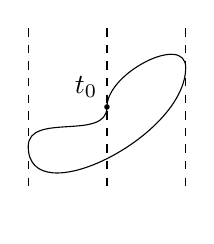
\begin{tikzpicture}
                            \fill (0,0) circle (1pt) node[above left] {$t_0$};
                            \draw (0,0) to[out=90,in=90] (1,0.5);
                            \draw (-1,-0.5) to[out=90,in=270] (0,0);
                            \draw (-1,-0.5) to[out=270,in=270] (1,0.5);
                            \draw[dashed] (0,1) -- (0,-1);
                            \draw[dashed] (1,1) -- (1,-1);
                            \draw[dashed] (-1,1) -- (-1,-1);
                        \end{tikzpicture}
                        \caption{\label{not-one-side}Три касательные}
                    \end{minipage}
                \end{figure}
            }
            }
        }
    }


    \section{Кривые в старших размерностях}
    Пусть $\gamma: [0, L] \map \R^n$ --- натурально параметризованная регулярная кривая, $\gamma' = v$.

    Так как $\angles{v, v} = 1$, то $\angles{v, v'} = 0$, $v'$ --- \emph{вектор кривизны}.
    \definition[Кривизна (без знака)]{Модуль вектора кривизны $k \bydef |v'| = |\gamma''|$.}
    \definition[(Главная) нормаль]{$N \bydef \frac{\gamma''}{|\gamma''|}$.}
    Если размерность объемлющего пространства на самом деле равна двум, то $N = \pm n$.

    \definition[Соприкасающаяся плоскость]{
        $\Lin(\gamma',\gamma'') = \Lin(v, N)$.
    }
    Потом обоснуем, что от данной плоскости кривая отходит медленнее всего;\ при $k = 0$ таких плоскостей много.
    \properties{
        \item $v \perp N, |v| = |N| = 1$.
        \item Кривизна $k$ сохраняется при движении.
%    \item $\dot{N} = -k v$.
%    \provehere{
%    Аналогично двумерному случаю: $\angles{v, N} = 0 \then \underbrace{\angles{\dot{v}, N}}_{k} + \langle v, \dot{N}\rangle = 0$.
%
%        $\langle N, N\rangle = 1 \then \langle N, \dot{N}\rangle = 0$, проекции $\dot{N}$ на $v$ и $N$ совпали с проекциями $-kv$.
%    }
    }
    Пусть $\tilde{\gamma}$ не натурально параметризована, $\tilde{\gamma} = \gamma \circ \phi$, где $\gamma$ уже параметризована натурально, здесь $\phi: \R \map \R$ --- гладкая перепараметризация ($s \coloneqq \phi' > 0$).

    \[\all{\tilde{\gamma}'(t) = \gamma'(\phi(t)) \cdot \phi'(t) \\ \phi'(t) = |\tilde{\gamma}'(t)| = s(t)} \then \tilde{\gamma}'(t) = s(t)\gamma'(\phi(t)) \qquad \tilde{\gamma}''(t) = s^2(t) \gamma''(\phi(t)) + s'(t)\gamma'(\phi(t)) = s^2 kN + s' v\]
    Таким образом, здесь тоже для соприкасающейся плоскости $\Lin(v, N) = \Lin(\gamma', \gamma'')$.

    В физике $\tilde{\gamma}''$ --- ускорение, и оно раскладывается в составляющие: $\overrightarrow{a} = \underbrace{\frac{|v|^2}{R}\overrightarrow{N}}_{\text{нормальная}} + \underbrace{|v|'\cdot \overrightarrow{v}}_{\text{тангенциальная}}$

    Из $\tilde{\gamma}'$ и $\tilde{\gamma}''$ можно найти $N, k, v: v = \tilde{\gamma}'$, и так как $\tilde{\gamma}'' = s^2 k N + s' v$, $k \ge 0, |N| = 1$, то $N$ тоже находится однозначно.

    Имеет место прежняя двумерная формула (но с модулем) $k = \frac{|\tilde{\gamma}' \wedge \tilde{\gamma}''|}{|\tilde{\gamma}'|^3}$, здесь $\wedge$ --- внешнее произведение.
    \ok
    Пусть $\gamma: [0, L] \map \R^n$ --- кривая в натуральной параметризации.
    \definition[Поворот кривой $\gamma$ в старших размерностях на отрезке $\lbrack a, b\rbrack \subset \lbrack 0, L\rbrack$]{
        $\int\limits_{a}^{b}k(\tau)\d\tau$.
    }
    Следовательно, в ненатуральной параметризации надо интегрировать $k |\tilde{\gamma}'|$.
    \precaution{
        Определение совсем не совпадает с определением поворота плоской кривой!
        У такой кривой $\begin{tikzpicture}[baseline=-4]
                            \draw[->] (0,0) to[out=45, in=225] (1,0);
        \end{tikzpicture}$ плоский поворот нулевой, а поворот в старших размерностях больше нуля (так как у кривизны нет знака).
    }
    \statement{
        $\angle(v(b), v(a)) \le \int\limits_{a}^{b}k\d\tau$.
        \provehere{
            $|v'| = k$, и $\abs{\int\limits_{a}^{b}v'\d\tau}\le\int\limits_{a}^{b}\abs{v'}\d\tau$.
            Вообще, поворот --- это длина кривой $v: [a, b] \map S^{n-1}$, а угол --- расстояние на сфере от $v(a)$ до $v(b)$.
        }
    }
    \theorem[Фенхель]{
        Пусть $\gamma$ --- регулярная замкнутая кривая.
        Тогда поворот $\gamma$ составляет хотя бы $2\pi$.
        \provehere{
            \indentlemma{
                Пусть даны три точки $A, B, C \in S^m$, такие, что $\underbrace{\angle(A, C)}_{\beta} + \underbrace{\angle(C, B)}_{\alpha} < \pi$.

                Тогда, понятное дело, $\angle(A, B) < \pi$, и есть кратчайшая дуга $\overset{\frown}{AC}$, отметим её середину $M$.
                Утверждается, что $\angle(C, M) < \frac{\pi}2$, то есть $C$ лежит в открытой полусфере с центром в $M$.
                \note{
                    Если знаки нестрогие, то не выполнено: можно взять $A, M, B, C$ на одной большой окружности:
                    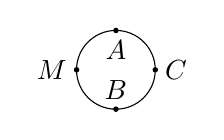
\begin{tikzpicture}[baseline=-4]
                        \draw(0,0) circle[radius=0.5];
                        \fill (-0.5,0) circle (1pt) node[left] {$M$};
                        \fill (0.5,0) circle (1pt) node[right] {$C$};
                        \fill (0,0.5) circle (1pt) node[below] {$A$};
                        \fill (0,-0.5) circle (1pt) node[above] {$B$};
                    \end{tikzpicture}.
                }
            }{
                Пусть $O$ --- центр сферы, достаточно показать, что $\langle OC, \underbrace{OB + OA}_{\upuparrows OM}\rangle > 0$.
                Действительно, $\angles{OC, OB} + \angles{OC, OA} = \cos \alpha + \cos \beta > \cos(\pi - \beta) + \cos \beta = 0$.
            }
            \indentlemma{\label{short}Пусть $\gamma: [a, b] \map S^m$ --- кривая, и $L(\gamma) < 2\pi$.
            Тогда $\Image(\gamma)$ лежит в некоторой открытой полусфере.
            }{
                Поделим кривую пополам: выберем $t_0 \in (a, b): L\left(\gamma\big|_{[a, t_0]}\right), L\left(\gamma\big|_{[t_0, b]}\right) < \pi$.
                Положим $A \coloneqq \gamma(a) = \gamma(b), B \coloneqq \gamma(t_0)$.
                Тогда $\forall C \in \Image(\gamma): \angle(A, C) + \angle(C, B) < \pi$, и все такие точки лежат в полусфере с центром в $M$ --- середине дуги $\overset{\frown}{AB}$.
            }
            \indent{\lemma{\label{ubiquitous}
            Вектор скорости регулярной замкнутой кривой не лежит ни в какой открытой полусфере.
            \provehere[Доказательство леммы]{
                От противного: пусть $\exists z \in S^{n-1}$, такой, что $\angles{z, v} > 0$.
                Тогда $\angles{\gamma(b) - \gamma(a), z} = \int\limits_{a}^{b}\angles{v, z} > 0$, то есть кривая не замкнута.
            }}}
            От противного: пусть поворот меньше $2\pi$, или же длина кривой, которую заметает вектор скорости $v: [a, b] \map S^{n - 1}$ меньше $2\pi$. Но тогда согласно~(\cref{short}) вектор скорости лежит в одной открытой полусфере, получаем противоречие с~(\cref{ubiquitous}).
        }
    }


    \section{Кривые в $\R^3$, кручение кривых}
    Пусть $\gamma: [0, L] \map \R^3$ --- кривая в натуральной параметризации, $k \ne 0$.
    Определения вектора скорости $v$, нормали $N$ и кривизны $k$ остались прежними.
    \definition[Бинормаль]{
        $b \coloneqq v \times N$. Так как $v \perp N$, то $(v, N, b)$ --- правый ортонормированный базис, $b$ --- перпендикуляр к соприкасающейся плоскости.
    }
    \note{
        $0 = \angles{v, b} \then 0 = \angles{k N, b} + \angles{v, b'}$ и $1 = \angles{b, b}$, откуда $\all{\angles{b', v} = 0 \\ \angles{b', b} = 0}$, то есть $b' \parallel N$.
    }
    \definition[Кручение]{
        Такое число $\tau$, что $b' = -\tau N$ ($\tau = -\angles{b', N}$).
    }
    Для регулярной кривой $\gamma$ с ненулевой кривизной $k$ получаем \emph{трёхмерный базис Френе}: гладкие $v, N, b$, \emph{кривизна} $k$ и \emph{кручение} $\tau$, такие, что выполняются формулы Френе:
    \[\dot{v} = k N \qquad \dot{b} = -\tau N \qquad \dot{N} = -k v + \tau b\]
    Последняя формула берётся из $\all{\langle\dot{N}, N\rangle = 0 \\ \langle\dot{N}, v\rangle = -\langle\dot{v}, N\rangle \\ \langle\dot{N}, b\rangle = -\langle\dot{b}, N\rangle}$.

    \theorem{
        Кручение нулевое $\tau = 0 \iff \gamma$ --- плоская кривая, $\Image(\gamma)$ лежит в некоторой плоскости.
        \provetwhen{
            Из формул Френе: $\dot{b} = 0$, то есть $b = b_0 = \const$.
            Заметим, что $\angles{\gamma, b_0}' = \angles{v, b_0} = 0$, то есть $\angles{\gamma, b_0} = \const$.
        }{
            Пусть $\Image(\gamma) \subset P \cong \R^2$. Тогда $v, N \parallel P$, и $b = v \times N = \const$ --- нормаль к $P$ (из непрерывности она не меняет направление).
            Значит, $\dot{b} = 0 \then \tau = 0$.
        }
    }

    \subsection{Скорость ухода от соприкасающейся плоскости}
    Помимо \emph{соприкасающейся плоскости} $\Lin(v, N)$, определяют также \emph{нормальную плоскость} $\Lin(N, b)$ (вектор скорости перпендикулярен ей) и \emph{спрямляющую плоскость} $\Lin(v, b)$ (кривизна в проекции на неё равна нулю).

    Запишем $\gamma'' = k N$, и $\gamma''' = k(-k v + \tau b) + \dot{k}N$.

    Теперь можно написать ряд Тейлора $\gamma(t) = \gamma(t_0) + v(t - t_0) + \frac{kN}{2}(t - t_0)^2 + \frac{\gamma'''}{6}(t - t_0)^3 + o((t - t_0)^3)$.
    Пусть $P$ --- соприкасающаяся плоскость, то есть плоскость, проходящая через $\gamma(t_0)$, и натянутая на $(v, N)$.

    Из ряда Тейлора получаем $\pm d(\gamma(t), P) = \frac{\angles{\gamma''', b}}{6} \cdot (t-t_0)^3 + o((t - t_0)^3) = \frac{k\tau}{6}(t - t_0)^3 + o((t - t_0)^3) = \bigO((t - t_0)^3)$, то есть порядок касания соприкасающейся плоскости $\ge 2$.
    \theorem{
        Пусть $\gamma$ --- кривая (необязательно в натуральной параметризации).
        Тогда $\tau = \dfrac{[\gamma', \gamma'', \gamma''']}{|\gamma' \times \gamma''|^2}$, где $[\_,\_,\_]$ --- смешанное произведение, то есть определитель матрицы, составленной из данных векторов (записанных в некотором ортонормированном базисе).
        \provehere{
            Натурально параметризуем: пусть $\gamma = \overline{\gamma}(\phi(t))$, где $|\overline{\gamma}'| = 1$, положим $s \coloneqq \phi'$.

            \indent{Ниже все аргументы у $s, \gamma$ и их производных --- $t$, а у остальных функций ($\overline{\gamma}, k, N, \tau$, и их производных) --- $\phi(t)$.}

            \gather{\gamma' = \overline{\gamma}' \cdot s = v \cdot s\\\gamma'' = v' \cdot s^2 + v \cdot s' = s^2 \cdot k N + vs'\\\gamma''' = 2 ss'\cdot kN + s^2 \cdot k'\cdot s \cdot N + s^2 k(-kv + \tau b)\cdot s + s''v + s'\cdot(kN)\cdot s}
            Используя антисимметричность смешанного произведения, получаем \[[\gamma', \gamma'', \gamma'''] = [v \cdot s, s^2 \cdot kN, s^2 k \tau bs] = s^6 k^2 \tau\]
            С другой стороны, $\abs{\gamma' \times \gamma''} = \abs{v \cdot s \times s^2 k N} = s^3 k$, откуда получается искомая формула для $\tau$.
        }
    }
    \newlection{6 ноября 2023 г.}


    \section{Базис Френе и кривизны в $\R^n$}
    \definition[$\gamma: I \map \R^n$ --- невырожденная кривая]{ $\gamma', \dots, \gamma^{(n - 1)}$ линейно независимы.}
    \theorem{
        Пусть $\gamma$ --- натурально параметризованная невырожденная кривая в $\R^n$.
        Тогда $\exists! v_1, \dots, v_n: I \map \R^n$ --- базис Френе, зависящий от времени, и $\exists!$ гладкие функции $k_1, \dots, k_{n-1}: I \map \R^n$, такие, что $k_1, \dots, k_{n-2} > 0, k_{n-1}$ имеет любой знак.
        При этом выполнены формулы Френе
        \numbers{
            \item $\gamma'(t) = v_1(t)$
            \item $\all{v_1' = k_1 v_2 \\ v_i' =  -k_{i-1}v_{i-1} + k_i v_{i+1} \text{ (при $2 \le i \le n-1$)} \\ v_n' = -k_{n-1}v_{n-1}}$.
            Это также можно записать в виде $v' = Kv$, где $K$ --- двухдиагональная антисимметричная матрица из кривизн.
            \item Базис $v_1, \dots, v_n$ --- правый ортонормированный.
        }
        \provehere{
            Рассмотрим набор производных $\gamma', \dots, \gamma^{(n-1)}$, по ним строится $v_1, \dots, v_{n-1}$ при помощи ортогонализации Грама --- Шмидта.
            Алгоритм возвращает ортонормированный базис какого-то гиперпространства коразмерности 1, оно единственным образом дополняется до ортонормированного правого базиса $\R^n$.
            По построению $v_i$ --- гладкие функции, причём $v_1 = \gamma_1$.

            Дальше по данному базису раскладываются вектора производных.
            Проверим, что соответствующие коэффициенты получаются нужного знака, и много кто --- нули: проверим соответствие (2).
            \[v_i' = c_{i,1}v_1 + \cdots + c_{i,n}v_n\]
            Так как $\angles{v_i,v_i} = 1$, то $\angles{v_i',v_i} = 0$. Так как $\angles{v_i,v_j} = 0$, то $\angles{v_i',v_j} = -\angles{v_i,v_j'}$.
            Таким образом, матрица $(c_{i,j})$ кососимметричная.
            $v_i \in \Lin(\gamma^{(1)}, \dots, \gamma^{(i)})$, откуда $v_i' \in \Lin(\gamma^{(1)},\dots,\gamma^{(i+1)}) = \Lin(v_1, \dots, v_{i +1})$.
            Отсюда получаем $c_{i,j} = 0$ для $j > i + 1$, и из кососимметричности это значит, что $c_{i,j} = 0$ для $|i - j| > 1$.

            Из ортогонализации Грама --- Шмидта $v_i = k \gamma^{(i)} + r_i$, где $k > 0, r_i \in \Lin(\gamma^{(1)}, \dots, \gamma^{(i-1)})$.
            Продифференцируем и скалярно домножим на $v_{i + 1}$.
            Слева получится $k_i = \angles{\dot{v}_i, v_{i + 1}}$, а справа $k\angles{\gamma^{(i + 1)}, v_{i + 1}} > 0$, так как $v_{i+1} \perp \dot{r}_i + \dot{k}\gamma^{(i)}$.
            Отсюда кривизны действительно положительны.

            Проверим однозначность определения базиса Френе. Пойдём индукцией: пусть $v_1, \dots, v_{i}$ однозначно определены. Почему $v_{i+1}$ однозначно определён?
            Из формул $v_{i+1} \perp \Lin(v_1, \dots, v_{i})$, $v_i' \in \Lin(v_1, \dots, v_{i+1})$. Производная $v_i'$ определена однозначно, значит, $\Lin(v_1, \dots, v_{i+1})$. определена, как $\Lin(v_1, \dots, v_i, v_i')$.
            Так как $k_i = \angles{v_i', v_{i+1}} > 0$, то направление $v_{i+1}$ определено однозначно. $v_n$ же определяется однозначно из того, что базис --- правый.
        }
    }
    \theorem{
        Пусть даны гладкие функции $k_1, \dots, k_{n-1}: I \map \R$, такие, что $k_1, \dots, k_{n-2} > 0$.
        Тогда существует (и единственна с точностью до движения) кривая с такими кривизнами.
        \provehere{
            Отметим произвольную точку, произвольно выберем правый ортонормированный базис $v_0 = v(0), v_1, \dots, v_{n-1}$.
            В матричной записи $v' = Kv$. Это линейное дифференциальное уравнение, имеет единственное решение при начальных данных $v_0, \dots, v_{n-1}$.

            Таким образом ищется функция $v(t)$, тогда $\gamma = p_0 + \int\limits_{t_0}^{t}v(\tau)\d \tau$.

            Заметим, что $(v^tv)' = (v')^t v + v^t v' = v^t K^t v + v^t K v = v^t\underbrace{(K^t + K)}_{0}v = 0$, откуда базис $v$ --- правый ортонормированный в любой момент времени, а не только в нулевой.
        }
    }


    \section{2-мерные поверхности в $\R^3$}
    Далее всё происходит в $\R^3$.
    \definition[Топологическая поверхность $\Sigma$]{
        Подмножество $\Sigma \subset \R^3$, которое может быть получено, как образ топологического вложения связного двумерного многообразия $f: M \hookrightarrow \R^3$.

        Топологичность вложения означает, что топология, индуцируемая с помощью $f$ топологией $\R^3$ совпадает с собственной топологией $M$.
    }
    \definition[Гладкая поверхность $\Sigma \subset \R^3$] {
        Поверхность $\Sigma$, которая локально может быть представлена, как график гладкой функции: $\forall p \in M$: можно ввести координатные оси $x,y,z$ с нулём в $p$, так, что $\exists \underset{\ni p}{U} \subset \R^3: \exists f: (\Omega \subset \R^2_{x,y})\underset{\text{гладко}}\map \R: \Sigma \cap U = \Gamma_f$ (здесь $\Gamma_f$ --- график $f$ в $\R^3_{x,y,z}$).
    }
    \definition[Регулярное отображение $r$]{
        Дифференциал $\d r$ невырожден (то есть размерность образа линейного оператора максимально возможная).
    }
    Невырожденность гладкого $r: \R^2 \map \R^3$ при введении базиса $(u, v)$ в $\R^2$ можно переформулировать так: $\der{r}{u} \times \der{r}{v} \ne 0$.

    \subsection{Локальная параметризация}
    В дальнейшем часто будут использоваться частные производные.
    Они будут обозначаться $r'_x$, или же $\der{r}{x}$.
    Также часто используется обозначение $r_x$, но мне оно не нравится, и я стараюсь его избегать.
    \theorem{\label{regular-param-sigma}
    Пусть $\Omega \subset \R^2$, пусть $r: \Omega \map \R^3$ --- регулярное (всегда подразумевается, что ещё и гладкое).
    Если $r: \Omega \map \R^3$ --- вложение, то $r(\Omega) \eqqcolon \Sigma$ --- гладкая поверхность.
    \provehere{
        Рассмотрим $r$ покоординатно: \[\vect{u\\v} \overset{r}\mapsto \vect{r_1(u, v) = x(u,v)\\r_2(u,v) =y(u,v)\\r_3(u,v)=z(u,v)}\]
        Так как дифференциал невырожден, то найдётся минор с ненулевым определителем.
        Без потери общности $\abs{\arr{cc}{x'_u & y'_u \\ x'_v & y'_v}} \ne 0$.

        Пусть $p = r(x_0)$. Из невырожденности дифференциала $\exist W \subset \Lin(x, y), V \subset \Lin(u, v)$ и обратное отображение $s: W \map V$, такое, что $(r_1, r_2) \circ s = \id$.
        Тогда $(r \circ s)(x, y) = (x, y, (r_3 \circ s)(x, y))$.
        Обозначим $f \coloneqq r_3 \circ s$; заметим, что $r(V)$ открыто в $\Sigma$, получаем, что $r(V)$ переписывается в виде $\Sigma \cap U$ для некоторого открытого $U \subset \R^3$.
    }
    }
    \definition[Регулярная параметризация поверхности $\Sigma$]{Отображение $r$, как в~(\cref{regular-param-sigma})}
    \note{
        Далеко не всякая поверхность в $\R^3$ гомеоморфна плоскости, например, у сферы $S^2 \subset \R^3$ нет регулярной параметризации.

        Тем не менее, существует локальная регулярная параметризация, которая получается из тех же соображений, что в теореме.
    }
    Пусть $r$ --- регулярная параметризация, как в теореме.
    Тогда $\exists r^{-1} \eqqcolon \phi: \Sigma \map \Omega$, оно называется \emph{картой}.

    \definition[Две эквивалентные регулярные параметризации $r_1: \Omega_1 \map \Sigma$ и $r_2: \Omega_2 \map \Sigma$]{
        $\exists$ гладкое регулярное $s: \Omega_1 \map \Omega_2$, такое, что $s^{-1}$ --- тоже гладкое регулярное, такое, что $r_1 = r_2 \circ s$.
    }
    % https://q.uiver.app/#q=WzAsMyxbMCwxLCJcXE9tZWdhXzEiXSxbMSwxLCJcXE9tZWdhXzIiXSxbMSwwLCJcXFNpZ21hIl0sWzAsMiwicl8xIl0sWzEsMiwicl8yIiwyXSxbMCwxLCJzIiwyXV0=
    \[\begin{tikzcd}[ampersand replacement=\&]
          \& \Sigma \\
          {\Omega_1} \& {\Omega_2}
          \arrow["{r_1}", from=2-1, to=1-2]
          \arrow["{r_2}"', from=2-2, to=1-2]
          \arrow["s"', from=2-1, to=2-2]
    \end{tikzcd}\]
    \exercise{
        Для гладкой поверхности локально любые две параметризации эквивалентны.
    }
    Пусть $r: \Omega \map \Sigma$ --- регулярная параметризация.

    \indent{Пусть $l: [0, 1] \map \Omega, l(t) = (t, v_0)$ --- путь с постоянной координатой $v_0$.
    Можно ввести координатные линии $r \circ l$, отвечающее линиям $r(t, v_0)$ и аналогично $r(u_0, t)$.

    Векторы скорости координатных линий $r'_u(t, v_0)$ и $r'_v(u_0, t)$.

    Пусть $\tilde{\gamma} = r \circ \gamma$. $\gamma$ регулярна $\iff$ $\tilde{\gamma}$ регулярна.
    Обратно можно получить $\gamma = \phi \circ \tilde{\gamma}$.
    }
    \statement{Пусть $f: \R^m \map \R^n$ --- гладкое отображение.

    Чтобы посчитать производную по направлению $v \in \R^m$ в $p_0 \in \Image(f)$, можно взять произвольную гладкую кривую $\gamma: (-\eps, +\eps) \map \R^m$, такую, что $\gamma(0) = p_0, \gamma'(0) = v$, тогда $(f \circ \gamma)'(0)$ --- искомая.
    \provehere{
        $(f \circ \gamma)'(0) = \d f(\gamma(0)) \cdot \d\gamma(0) = \d f(p_0) \cdot v$.
        Это выражение не зависит от пути $\gamma$, и является фактически определением производной по направлению.
    }
    }
    \definition[Касательное пространство к $\Sigma$ в точке $p = r(x)$]{
        $T_p(\Sigma) = \d_x r(\R^2)$.
    }
    Касательное пространство можно рассматривать, как линейное пространство, или аффинное пространство в $\R^3$.

    \statement{
        Касательное пространство не зависит от параметризации.
        \provehere{
            Можно определить эквивалентным образом: касательное пространство $T_p(\Sigma) = \{\text{векторы скорости гладких кривых, проходящих через точку $p$}\}$
        }
    }
    Касательная плоскость --- линейное пространство, натянутое на векторы $\der{r}{u}$ и $\der{r}{v}$ --- стандартный базис в касательном пространстве.
    $\der{r}{u} = r'_u = \d r(1, 0), \der{r}{v} = r'_v = \d r(0, 1)$.
    \newlection{13 ноября 2023 г.}

    \subsection{Гладкие функции на поверхности}
    Определим гладкую функцию $f: \Sigma \map \R$ из поверхности в прямую.
    \definition[Функция $f$ гладкая]{
        $\forall p \in \Sigma: \exists U \ni p$, и карта, такая, что $f$ --- гладкая в карте $U$, то есть $\exists r: \Omega \map U: f \circ r$ --- гладкая.
    }
    \statement{
        Условие гладкости $f: \Sigma \map \R$ равносильно следующим:
        \numbers{
            \item $f$ гладкая в любой карте.
            \item $\exists F: (\subset \R^3) \map \R$ --- продолжение $f$, гладкое в окрестности любой точки.
        }
        \provehere{\down
        \numbers{
            \item Отображение перехода между картами $s$ --- регулярно, и $s^{-1}$ --- тоже регулярно.
            \note{
                Из теоремы об обратном отображении $s$ --- регулярная биекция.
            }
            \item Если поверхность локально задаётся графиком $\Sigma = (x, y, h(x, y))$, то можно определить $F(x, y, z) = f(x, y, h(x, y))$.
            Обратно, если $F: (\subset \R^3) \map \R$ гладкое, то гладко и $F\big|_{\Sigma}$.
        }
        }
    }

    \subsection{Производная по направлению}
    Пусть взяты точка в поверхности $p \in \Sigma$ и касательный вектор $X \in T_p(\Sigma)$.

    Пусть $f: \Sigma \map \R$ --- гладкая функция, пусть $\tilde{\gamma}: (-\eps, +\eps) \map \Sigma$ --- кривая на поверхности.
    Пусть $p \coloneqq \tilde{\gamma}(0), \tilde{\gamma}'(0) = X$.
    Тогда
    \numbers{
        \item $f \circ \tilde{\gamma}$ --- гладкая (скалярная) функция.
        \item $(f \circ \tilde{\gamma})'(0)$ --- не зависит от $\tilde{\gamma}$.
        \item Для всякой параметризации $r: \Omega \map \R^3$: $(f \circ \tilde{\gamma})'(0) = X_1 \der{f \circ r}{u} + X_2 \der{f \circ r}{v}$, где $X_1, X_2$ --- координаты $X$ в базисе $r'_u, r'_v$.
    }
    \provebullets{
        \item[1.] Композиция гладких функций --- гладкая (можно продолжить $f$ до $F: \R^3 \map \R$).
        \item[2.] Следует из следующего.
        \item[3.] Пусть $r: \Omega \map \Sigma$ --- параметризация, и $\tilde{\gamma} = r \circ \gamma$, где $\gamma: (-\eps, +\eps) \map \Omega$.

        Обозначим $\gamma(t) = \vect{u(t) \\ v(t)}$, получим $(f \circ \tilde{\gamma})'(0) = \left(f \circ r \circ \vect{u \\ v}\right)'(0) = (f \circ r)'_u \cdot u'(0) + (f \circ r)'_v \cdot v'(0)$.

        При этом действительно $\tilde{\gamma}'(0) = r'\vect{u \\ v}(0) \cdot \vect{u'(0) & v'(0)}$, то есть $u'(0), v'(0)$ --- координаты $X = \tilde{\gamma}'(0)$ в базисе $r'_u, r'_v$.
    }
    $X_1 (f \circ r)'_u + X_2 (f \circ r)'_v$ называется \emph{производной функции $f: \Sigma \map \R$ в точке $p \in \Sigma$ по направлению} $X \in T_p(\Sigma)$, обозначается $X_p(f)$.

    \definition[$f: \Sigma \map \R^3$ --- гладкая функция]{
        $f$ --- гладкая покоординатно.
    }
    Пусть теперь есть две поверхности $\Sigma_1$ и $\Sigma_2$.

    Если $\Image(\tilde{f}) \subset \Sigma_2$, то $\tilde{f}$ --- гладкая функция $\Sigma_1 \map \Sigma_2$ из одной поверхности в другую.

    Можно рассмотреть соответствующую $f: \Omega_1 \map \Omega_2$
% https://q.uiver.app/#q=WzAsNCxbMCwxLCJcXE9tZWdhXzEiXSxbMCwwLCJcXFNpZ21hXzEiXSxbMSwwLCJcXFNpZ21hXzIiXSxbMSwxLCJcXE9tZWdhXzIiXSxbMCwzLCJmIiwyXSxbMCwxLCJyXzEiLDJdLFsxLDIsIlxcdGlsZGV7Zn0iLDJdLFszLDIsInJfMiJdXQ==
    \[\begin{tikzcd}[ampersand replacement=\&]
    {\Sigma_1}
          \& {\Sigma_2} \\
          {\Omega_1} \& {\Omega_2}
          \arrow["f"', from=2-1, to=2-2]
          \arrow["{r_1}"', from=2-1, to=1-1]
          \arrow["{\tilde{f}}"', from=1-1, to=1-2]
          \arrow["{r_2}", from=2-2, to=1-2]
    \end{tikzcd}\]
    \statement{$\tilde{f}$ --- гладкая $\iff f$ гладкая в некоторой карте.
    \provehere{
        \bullets{
            \item[$\then$] Рассмотрим хорошую карту, в которой параметризации --- графики $(x, y, h(x, y))$.
            В ней $f$ действительно гладкая.
            \item[$\when$] Из коммутативности диаграммы $\tilde{f} = r_2 \circ f \circ r_1^{-1}$.
        }
    }
    }
    Пусть $\tilde{f}: \Sigma_1 \map \Sigma_2$ --- гладкая.
    Посчитаем производную по направлению, рассматривая $\tilde{f}$, как функцию в $\R^3$.
    Пусть $X \in T_p(\Sigma_1)$.
    Утверждается, что $X(\tilde{f}) \in T_{\tilde{f}(p)}(\Sigma_2)$.

    \definition[Дифференциал $\tilde{f}$ в точке $p$ по направлению $X$]{
        $\d_p\tilde{f}(X) \bydef X(\tilde{f})$.
    }
    Дифференциал в точке $p$ --- линейное отображение $T_p(\Sigma_1) \map T_{\tilde{f}(p)}(\Sigma_2)$.
% https://q.uiver.app/#q=WzAsMyxbMCwwLCJcXFNpZ21hXzEiXSxbMSwwLCJcXFNpZ21hXzIiXSxbMiwwLCJcXFNpZ21hXzMiXSxbMCwxLCJcXHRpbGRle2Z9Il0sWzEsMiwiXFx0aWxkZXtnfSJdLFswLDIsIlxcdGlsZGV7aH0iLDIseyJjdXJ2ZSI6M31dXQ==
    \[\begin{tikzcd}[ampersand replacement=\&]
    {\Sigma_1}
          \& {\Sigma_2} \& {\Sigma_3}
          \arrow["{\tilde{f}}", from=1-1, to=1-2]
          \arrow["{\tilde{g}}", from=1-2, to=1-3]
          \arrow["{\tilde{h}}"', curve={height=18pt}, from=1-1, to=1-3]
    \end{tikzcd}\]
    Дифференциал композиции равен произведению дифференциалов $\d\tilde{g} \circ \d\tilde{f} = \d \tilde{h}$.

% https://q.uiver.app/#q=WzAsNCxbMCwxLCJcXE9tZWdhXzEiXSxbMCwwLCJcXFNpZ21hXzEiXSxbMSwwLCJcXFNpZ21hXzIiXSxbMSwxLCJcXE9tZWdhXzIiXSxbMCwzLCJmIiwyXSxbMCwxLCJyXzEiLDJdLFsxLDIsIlxcdGlsZGV7Zn0iLDJdLFszLDIsInJfMiJdXQ==
    \[\begin{tikzcd}[ampersand replacement=\&]
    {\Sigma_1}
          \& {\Sigma_2} \\
          {\Omega_1} \& {\Omega_2}
          \arrow["f"', from=2-1, to=2-2]
          \arrow["{r_1}"', from=2-1, to=1-1]
          \arrow["{\tilde{f}}"', from=1-1, to=1-2]
          \arrow["{r_2}", from=2-2, to=1-2]
    \end{tikzcd}\]
    Частным случаем этого утверждения является $\d \tilde{f} \circ \d r_1 = \d r_2 \circ \d f$.
    \definition[$\tilde{f}$ регулярно]{
        $\d \tilde{f}$ невырожден (здесь эквивалентно: $f$ регулярно в любой карте).
    }


    \section{Первая квадратичная форма поверхности}
    Имеется соответствие между квадратичными и билинейными симметричными формами: сужение билинейной формы на диагональ --- квадратичная форма ($B(x, x) = Q(x)$), и билинейную форму можно восстановить по квадратичной.
    Поэтому в будущем мы будем использовать слова квадратичной и билинейной формы взаимозаменяемо.

    После выбора базиса $(e_1, \dots, e_n) \in V$ для билинейной формы можно записать матрицу $[B] = (b_{i,j})_{i,j} = (B(e_i,e_j))_{i,j}$.

    $I$ квадратичная форма определяется для параметризации $r: \Omega \map \Sigma$.
    Положим $I_x: \R^2\times\R^2 \map \R$, $I_x(X, Y) \bydef \angles{\d_x r(X), \d_x r(Y)}_{\R^3}$.
    Это билинейная симметричная форма.
    \definition[$I$ квадратичная форма в $x \in \Omega$]{
        Квадратичная форма, отвечающая сужению на диагональ: $I_x(X) \bydef I_x(X, X)$.
    }
    Матрица квадратичной формы $[I_x] = (g_{i,j})_{i,j} = (\angles{\d r(e_i), \d r(e_j)})_{i,j}$ --- \emph{метрический тензор}.

    Имеются установленные буквенные обозначения $[I_x] = \vect{E & F \\ F & G}$.
    А именно, \[E(u, v) \coloneqq \angles{r'_u(u, v), r'_u(u, v)}, F(u, v) \coloneqq \angles{r'_u(u, v), r'_v(u, v)}, G(u, v) \coloneqq \angles{r'_v(u, v), r'_v(u, v)}\]

    Разложим в этом базисе $X = (X_1, X_2)$ и $Y = (Y_1, Y_2)$, получаем $I(X, Y) = X_1 E Y_1 + (X_1 F Y_2 + X_2 F Y_1) + X_2 G Y_2$.

    \examples[Вычисления, связанные первой с квадратичной формой]{
        \item Длина вектора $X$ --- это $\sqrt{I(X, X)}$, $\cos(\angle(X, Y)) = \frac{I(X, Y)}{\sqrt{I(X)}\sqrt{I(Y)}}$.

        \item Пути на поверхности $\tilde{\gamma} = r \circ \gamma$ сопоставляется его длина $L(\tilde{\gamma}) = \int\sqrt{I(\gamma',\gamma')}\d t$

        \item     Ортонормированному базису $(u, v)$ соответствует базис $r'_u, r'_v$.
        Площадь поверхности $r(\Omega)$ равна $\int\limits_{\Omega}\sqrt{EG - F^2}\d s$ (это было обосновано на матанализе, $EG - F^2 = \det I$).
    }

    \subsection{I форма при замене координат}
    Пусть $r: \Omega_1 \map \Sigma, r^*: \Omega_2 \map \Sigma$ --- две параметризации $\Sigma$, отображение перехода между картами $s$.
% https://q.uiver.app/#q=WzAsMyxbMCwxLCJcXE9tZWdhXzEiXSxbMiwxLCJcXE9tZWdhXzIiXSxbMSwwLCJcXFNpZ21hIl0sWzEsMCwicyJdLFswLDIsInIiXSxbMSwyLCJyXioiLDJdXQ==
    \[\begin{tikzcd}[ampersand replacement=\&]
          \& \Sigma \\
          {\Omega_1} \&\& {\Omega_2}
          \arrow["s", from=2-3, to=2-1]
          \arrow["r", from=2-1, to=1-2]
          \arrow["{r^*}"', from=2-3, to=1-2]
    \end{tikzcd}\]
    Обозначим за $I$ квадратичную форму, отвечающую $r$, за $I^*$ --- отвечающую $r^*$.

    При замене параметризации одна форма выражается через другую: $I^*(v, w) = I(\d s(v), \d s(w))$.
    В координатной форме (считая, что базисы согласованы: $s$ переводит базис $I^*$ в базис $I$)
    \[[v]^t[I^*][w] = ([\d s][v])^t[I] \cdot [\d s][w] = [v^t]([\d s]^t [I][\d s])[w] \qquad [I^*] = [\d s]^t [I] [\d s]\]
    \example{
        Рассмотрим две разные параметризации плоскости --- в декартовых и полярных координатах.
        \numbers{
            \item В декартовых $r(u, v) = (u, v, 0)$. $I = \vect{1 & 0 \\ 0 & 1}$
            \item В полярных $r(\rho, \phi) = (\rho \cos(\phi), \rho \sin(\phi), 0)$.
            $\der{r}{\rho} = (\cos \phi, \sin \phi)$, $\der{r}{\phi} = (-\rho\sin\phi, \rho\cos\phi)$.

            Получаем $\d s = \vect{\cos \phi & -\rho \sin \phi \\ \sin \phi & \rho \cos \phi}$, и $[\d s]^t \cdot [\d s] = \vect{1 & 0 \\ 0 & \rho^2}$.
            Отсюда $[I^*] = \vect{1 & 0 \\ 0 & \rho^2}$.
        }
    }

    \subsection{Изометрии}
% https://q.uiver.app/#q=WzAsNCxbMCwxLCJcXE9tZWdhXzEiXSxbMCwwLCJcXFNpZ21hXzEiXSxbMSwwLCJcXFNpZ21hXzIiXSxbMSwxLCJcXE9tZWdhXzIiXSxbMCwzLCJmIiwyXSxbMCwxLCJyXzEiLDJdLFsxLDIsIlxcdGlsZGV7Zn0iLDJdLFszLDIsInJfMiJdXQ==
    \[\begin{tikzcd}[ampersand replacement=\&]
    {\Sigma_1}
          \& {\Sigma_2} \\
          {\Omega_1} \& {\Omega_2}
          \arrow["f"', from=2-1, to=2-2]
          \arrow["{r_1}"', from=2-1, to=1-1]
          \arrow["{\tilde{f}}"', from=1-1, to=1-2]
          \arrow["{r_2}", from=2-2, to=1-2]
    \end{tikzcd}\]

    Бывают такие поверхности, что их можно отобразить друг в друга, при этом длины соответствующих векторов не будут меняться.
    Например, квадрат скатать в цилиндр, или конус развернуть в кусок плоскости.
    \definition[Гладкое $\tilde{f}: \Sigma_1 \map \Sigma_2$ --- изометрия]{
        $\d \tilde{f}$ сохраняет скалярное произведение $\angles{\_,\_}$: $\forall V, W \in T_p(\Sigma_1): \angles{V, W} = \angles{\d_p \tilde{f}(V), \d_p\tilde{f}(W)}$.
    }
    Если параметризации используют одну карту --- например, вторая параметризация равна $r_2 = \tilde{f} \circ r_1$ --- то матрицы первых форм равны: $[I]^{r_1} = [I]^{r_2}$.
    В общем случае $[I]^{r_1} = [\d f]^t [I]^{r_2} [\d f]$.
    \example{
        Конус над любой кривой локально изометричен плоскости.
        \provehere{
            Пусть $\gamma_0: [0, 1] \map \R^2 \subset \R^3$ --- некоторая (гладкая регулярная) кривая, $O \in \R^3$ --- точка вне плоскости, содержащей $\Image(\gamma_0)$.

            Конусом над $\gamma_0$, по-видимому, называется подмножество $\R^3$, состоящее из лучей $\defset{OX}{X \in \Image(\gamma_0)}$.
            В вершине конуса, очевидно, есть излом поэтому следует рассматривать открытые лучи, не включающие точку $O$.

            Подвинем точки вдоль лучей, так, чтобы они все лежали на единичной сфере с центром в $O$; иначе говоря, пусть $\gamma(t) = O + \frac{\gamma_0(t) - O}{|\gamma_0(t) - O|}$.
            Конусы над $\gamma$ и над $\gamma_0$ совпадают; можно считать, что $\gamma$ натурально параметризована.

            Теперь конус задаётся параметризацией $r(\rho, t) = O + \rho \cdot (\gamma(t) - O)$. $\der{r}{\rho} = \gamma(t) - O, \der{r}{t} = \rho \cdot \gamma'(t)$.
            В такой параметризации первая квадратичная форма оказывается такой же, как и у параметризации плоскости в полярных координатах --- $\vect{1 & 0 \\ 0 & \rho^2}$. $\angles{\der{r}{\rho}, \der{r}{t}} = 0$, так как $\langle \gamma(t) - O, \gamma(t) - O \rangle = \const$.}
    }
    Пусть $p, q \in \Sigma$, тогда расстояние между точками $d(p, q) = \inf\defset{L(\tilde{\gamma})}{\tilde{\gamma}: [0, 1] \map \Sigma, \tilde{\gamma}(0) = p, \tilde{\gamma}(1) = q}$.
    Это \emph{внутренняя метрика поверхности}.

    Внутренняя метрика, вообще говоря, не совпадает с внешней --- между диаметрально противоположными точками $S^1$ расстояние внешнее --- 2, внутреннее --- $\pi$.


    \section{Вторая квадратичная форма}
    Первая форма не менялась при изометриях, а вторая, наоборот, будет говорить, как поверхность изогнута в $\R^3$ --- на какой параболоид она больше всего похожа.

    Зафиксируем параметризацию $r: \Omega \map \Sigma$, определим единичную нормаль $n \coloneqq \frac{r'_u \times r'_v}{|r'_u \times r'_v|}$ в точке $r(x)$, $x \in \Omega$.
    \definition[Вторая квадратичная форма]{$\II_x(v, w) = \angles{\d_x^2 r(v, w), n}$.}
    Коэффициенты матрицы второй формы обозначают так: $[\II] = \vect{L & M \\ M & N}$, где $L = \angles{r''_{u,u}, n}, M = \angles{r''_{u,v}, n}, N = \angles{r''_{v,v}, n}$.
    \theorem{
        Можно рассмотреть нормаль, как гладкую функцию $\Omega \map (S^2 \subset \R^3)$. Утверждается, что $\II(v, w) = -\angles{\d r(v), \d n(w)}$.
        \provehere{
            $\d r(v)$ лежит в касательной плоскости, поэтому $\angles{\d r(v), n} = 0$.
            Дифференцируя по $w$, получаем
            $\angles{\d^2 r(v, w), n} + \angles{\d r(v), \d n(w)} = 0$.
        }
    }
    \newlection{20 ноября 2023 г.}

    \subsection{Специальные координаты. Соприкасающийся параболоид}
    Пусть $\Sigma$ --- поверхность, $p \in \Sigma$ --- точка.
    Выберем ортонормированный базис $x = f_1, y = f_2$ в $T_p \Sigma$.
    Можно выбрать такую окрестность $U \ni p$, что $\Sigma \cap U$ --- график $(x, y, f(x, y))$, причём третья ось направлена перпендикулярно $T_p\Sigma$.

    Тогда $r'_x(0) = (1, 0, f'_x) \in T_p\Sigma$ и $r'_y(0) = (0, 1, f'_y) \in T_p\Sigma$, и так как $T_p\Sigma$ натянуто на первые две оси, то $f'_x = f'_y = 0$.

    Иными словами, $\d f = 0$, и $n(0) = (0, 0, 1)$.
    Дифференцируя далее, получаем \[r''_{x,x}(0) = (0, 0, f''_{x,x})\qquad r''_{x,y}(0) = (0, 0, f''_{x,y})\qquad r''_{y,y}(0) = (0, 0, f''_{y,y})\]
    Записав коэффициенты $\II$ формы $L = \angles{r''_{x,x}, n} = f''_{x,x};~M = f''_{x,y};~N = f''_{y,y}$, получаем матрицу Гессе $H = \vect{f''_{x,x} & f''_{x,y} \\ f''_{x,y} & f''_{y,y}}$

    Из формул Тейлора $f(x, y) = \frac{1}{2}(Lx^2 + 2Mxy + Ny^2) + o(x^2 + y^2)$.
    Определим соприкасающийся параболоид $z = \frac{1}{2}(Lx^2 + 2Mxy + Ny^2)$, он касается поверхности (касание второго порядка).

    Оси координат $x, y$ можно так повернуть, чтобы смешанная производная $\der{}{y}\der{}{x}f = f''_{x,y}$ была равна нулю, тогда параболоид имеет вид $z = Ax^2 + By^2$.
    Гессиан в этих координатах имеет вид $\vect{L & 0 \\ 0 & N}$, и данные значения $L, N$ называются $k_1, k_2$ --- \emph{главные кривизны}, а сами координаты, в которых гессиан имеет такой вид --- \emph{специальные}.

    Если $k_1 \ne k_2$, то главные направления определены с точностью до перестановки осей, иначе матрица Гессе диагональна, и все направления главные.
    \definition[Гауссова кривизна]{ Произведение главных кривизн: $K \bydef k_1 \cdot k_2$.}
    \definition[Средняя кривизна]{ Полусумма главных кривизн, $\frac{k_1 + k_2}2$.}

    В специальных координатах векторы $r'_x, r'_y$ --- \emph{главные направления} --- образуют ортонормированный базис в $T_p\Sigma$~(\cref{veingarten-eigenvalues}).

    \definition[Эллиптическая точка]{
        Кривизны в ней одного знака, и не равны нулю.
    }
    \definition[Гиперболическая точка]{
        Кривизны в ней разного знака. Ещё такую точку называют \emph{седловая}.
    }
    \definition[Омбилическая точка]{
        Кривизны равны.
    }
    \definition[Параболическая точка]{
        Ровно одна из кривизн равна нулю.
    }
    \definition[Точка уплощения]{
        Обе кривизны равны нулю.
    }
    \ok
    На пространстве $(V, \angles{\_, \_})$ билинейной форме $B(x, y)$ по лемме Рисса соответствует линейный оператор $A: V \map V$, такой, что $B(x, y) = \angles{x, Ay}$.

    Если базис $e_1, \dots, e_n$ ортонормирован, то матрицы $[A] = [B]$ равны.
    Иначе $[B] = [G][A]$, где $[G]$ --- матрица Грама ($[G]$ симметрична).

    $[X]^t[B][Y] = [X]^t[G][AY]$.

    \fact{
        $[B]$ --- симметрическая матрица ($B$ --- симметричная форма) $\iff A$ --- самосопряжена.
        \provehere{
            $\angles{x, Ay} = [x]^t[G][A][y] = [x]^t[G][A][G]^{-1}[G][y] = \angles{([G][A][G]^{-1})^t[x], [y]}$, откуда $[A]$ самосопряжена $\iff ([G][A][G]^{-1})^t = [A] \iff [G][A] = ([G][A])^t$.
        }
    }
    \corollary{
        В ортонормированном базисе матрица самосопряжённого оператора симметрична.
        \provehere{
            В ортонормированном базисе $[G] = E$.
        }
    }

    \subsection{Гауссово отображение}
    Пусть $\Sigma \subset \R^3$ --- поверхность.
    \definition[Гауссово отображение]{ Непрерывное $\hat{n}: \Sigma \map S^2$, такое, что $\forall p \in \Sigma: \hat{n}(p) \perp T_p\Sigma$, $\abs{\hat{n}(p)} = 1$.}
    Если поверхность ориентируема, то $\hat{n}$ можно задать на всей поверхности, но нас будет интересовать задание в карте.

    Пусть $r: \Omega \map \Sigma$ --- параметризация, тогда можно определить $n(u, v) \coloneqq \frac{r'_u \times r'_v}{|r'_u \times r'_v|}$.
% https://q.uiver.app/#q=WzAsMyxbMCwxLCJcXE9tZWdhIl0sWzAsMCwiXFxTaWdtYSJdLFsxLDAsIlNeMiJdLFswLDEsInIiXSxbMSwyLCJcXGhhdHtufSJdLFswLDIsIm4iLDJdXQ==
    \[\begin{tikzcd}[ampersand replacement=\&]
          \Sigma \& {S^2} \\
          \Omega
          \arrow["r", from=2-1, to=1-1]
          \arrow["{\hat{n}}", from=1-1, to=1-2]
          \arrow["n"', from=2-1, to=1-2]
    \end{tikzcd}\]

    \subsection{Оператор Вайнгартена}
    Пусть $p \in \Sigma$.
    Посмотрим на $\d_p \hat{n}: T_p\Sigma \map T_{\hat{n}(p)}S^2$.
    Получается, в точке $p$ касательные пространства к $\Sigma$ и $S^2$ совпадают (как векторные пространства), так как у них общая нормаль $\hat{n}(p)$.

    Если их отождествить, то можно считать, что $\d_p\hat{n}: T_p\Sigma \map T_p\Sigma$.
    \definition[Оператор Вайнгартена]{
        $S \bydef -\d_p\hat{n}: T_p\Sigma \map T_p\Sigma$.
    }
    Определим билинейную форму $\hat{\II}: T_p\Sigma \times T_p\Sigma \map \R, \hat{\II}(v, w) = \angles{v, S(w)} = -\angles{v, \d_p\hat{n}(w)}$.
    Определение не использует никакую конкретную параметризацию ($\hat{n}$ в каждой точке определяется с точностью до знака, и если ориентация фиксирована, то однозначно).
    \theorem{
        Пусть $r: \Omega \map \Sigma$ --- произвольная параметризация, пусть $p = r(x)$.
        Тогда $\forall v, w \in \R^2: \II(v, w) = \hat{\II}(\d_x r(v), \d_x r(w))$.
        \provehere{
            Используем $\II(v, w) = -\angles{\d r(v), \d n(w)}$, и $n = \hat{n} \circ r$.
            Получаем \[\II_x(v, w) = \angles{\d_x r(v), -\d_p\hat{n}\cdot\d_x r(w)}\qedhere\]
        }
    }
    \corollary{\down
    \numbers{
        \item $\hat{\II}$ симметрична, поэтому оператор Вайнгартена самосопряжён.
        \item $[\II]_{u, v} = [\hat{\II}]_{r'_u, r'_v}$.
        \item По-прежнему в любой параметризации $[\hat{\II}]_{r'_u,r'_v} = [I]_{u,v} \cdot [S]_{r'_u,r'_v}$ --- здесь используется, что $[I]_{u,v}$ --- матрица Грама для базиса $r'_u$ и $r'_v$.
        \item Пусть есть две параметризации
% https://q.uiver.app/#q=WzAsMyxbMCwxLCJcXE9tZWdhXzEiXSxbMiwxLCJcXE9tZWdhXzIiXSxbMSwwLCJcXFNpZ21hIl0sWzAsMiwicl8xIl0sWzEsMiwicl8yIiwyXSxbMSwwLCJzIl1d
        \[\begin{tikzcd}[ampersand replacement=\&]
              \& \Sigma \\
              {\Omega_1} \&\& {\Omega_2}
              \arrow["{r_1}", from=2-1, to=1-2]
              \arrow["{r_2}"', from=2-3, to=1-2]
              \arrow["s", from=2-3, to=2-1]
        \end{tikzcd}\]
        Тогда $r_2 = r_1 \circ s$ и $[\II^{r_2}] = [\d s]^t [\II^{r_1}][\d s]$.
    }
    }
    \theorem{
        Пусть $\Omega$ --- линейно связно, и есть параметризация $r: \Omega \map \R^3$. \[\II \equiv 0 \iff r(\Omega) \text{--- часть плоскости}\]
        \provewthen{
            Для плоскости $n \equiv \const\then\d n \equiv 0\then \II \equiv 0$.
        }{
            Оператор Вайнгартена $S \equiv 0 \then \d \hat{n} \equiv 0 \then n = n_0 = \const$.
            Любая кривая $\gamma: [0, 1] \map \Sigma$ на поверхности перпендикулярна этой нормали во всякой своей точке.
            Функция высоты $H = \angles{\_, n_0}$ постоянна во всех точках кривой.
        }
    }
    \proposal{\label{veingarten-eigenvalues}
    Собственные числа оператора Вайнгартена --- главные кривизны (и они отвечают собственным векторам --- векторам, лежащим на главных направлениях).
    \provehere{
        Рассмотрим специальные координаты.
        В них $\vect{k_1 & 0 \\ 0 & k_2} = [\II]_{u,v} = [\hat{\II}]_{r'_u, r'_v}$, и так как $r'_u, r'_v$ --- ортонормированный базис, то $[S]_{r'_u, r'_v} = [\II]_{u,v} = \vect{k_1 & 0 \\ 0 & k_2}$.
    }
    }
    Из предложения следует, что так как оператор Вайнгартена самосопряжён, то у него существует ортонормированный базис из собственных векторов с вещественными собственными числами, а именно --- если $k_1 \ne k_2$, то главные направления перпендикулярны (если $k_1 = k_2$, то все направления --- главные).
    
    Пусть $r: \Omega \map \Sigma, x \in \Omega, p = r(x)$.
    \theorem[Родриг]{\down
    \numbers{
        \item Бескоординатная формулировка: $v \in T_p(\Sigma)$ на главном направлении $\iff \d\hat{n}(v)\parallel v$, причём если это так, то $\d\hat{n}(v) = -k_1 v$ или же $\d\hat{n}(v) = -k_2 v$.
        \item Для $\xi \in \R^2$: $\d r(\xi)$ на главном направлении $\iff \d r(\xi) \parallel \d n(\xi)$, причём если это так, то $\d n(\xi) = -k_{1}\cdot\d r(\xi)$ или $\d n(\xi) = -k_2 \cdot \d r(\xi)$.
    }
    \provenumbers{
        \item Это определение собственного вектора, а $S = -\d\hat{n}$.
        \item Из предыдущего $\d r(\xi)$ на главном направлении $\iff \d\hat{n}(\d r(\xi)) \parallel \d r(\xi)$.
        Теперь заметим, что $\d n(\xi) = \d\,(\hat{n} \circ r)(\xi) = \d\hat{n}\d r(\xi)$.
    }
    }
    \definition[Нормальное сечение с началом в точке $p$ и направлением $v \in T_p\Sigma$]{
        Пересечение $\Sigma \cap P(p, n(p), v)$, здесь $P(p, n(p), v)$ --- плоскость, проходящая через $p$, и натянутая на векторы нормали $n(p)$ и $v$.
    }
    В окрестности $p$ нормальное сечение --- кривая.

    Далее в определениях считаем, что во всех точках непрерывно выбрана нормаль $\hat{n}: \Sigma \map S^2$ (крышка иногда будет опускаться, если понятно из контекста).
    \definition[Кривизна поверхности в направлении вектора $v \in T_p\Sigma$]{
        Кривизна нормального сечения --- гладкой регулярной кривой $\gamma_v$ --- со знаком $+$, если нормаль к кривой $\gamma_v$ сонаправлена с $\hat{n}$, и $-$ иначе.
        Обозначается $k_n(v)$

        Иными словами, пусть $\gamma_v$ --- натурально параметризованная кривая, проходящая нормальное сечение: $\gamma_v' \upuparrows v$, $\gamma_v(0) = p$.
        Тогда $k_n(v) \bydef k_{\gamma_v}(0) \cdot \angles{N_{\gamma_v}(0), \hat{n}(p)} = \angles{\gamma''(0), \hat{n}(p)}$.
    }
    Теперь пусть $\tilde{\gamma}: [a, b] \map \Sigma$ --- натурально параметризованная кривая.
    Запишем $\tilde{\gamma}'' = k_{\tilde{\gamma}} \cdot N_{\tilde{\gamma}}$.

    \definition[Нормальная кривизна $\tilde{\gamma}$]{
        $k_n(\tilde{\gamma}) \coloneqq \angles{\tilde{\gamma}'', \hat{n}} = k_{\tilde{\gamma}} \cos(N, \hat{n})$.
    }
    \definition[Геодезическая кривизна $\tilde{\gamma}$]{
        $k_g$ --- модуль проекции $\tilde{\gamma}''$ на $T_p\Sigma$.
    }
    Фактически, вектор кривизны был разложен на нормальную и касательную составляющие, только нормальная со знаком, и касательная --- без.
    $k_g = \abs{\tilde{\gamma}'' - k_n \hat{n}}$.
    По теореме Пифагора $k_{\tilde{\gamma}} = \sqrt{k^2_n(\tilde{\gamma}) + k^2_g(\tilde{\gamma})}$.
    \definition[Геодезическая кривая $\gamma$]{ Такая кривая, что $k_g(\gamma) \equiv 0$.}

    \subsection{Выражение нормальной кривизны через квадратичные формы}
    Пусть $\tilde{\gamma}: [0, 1] \map \Sigma$ --- кривая на поверхности.
    Введём $\gamma: [0, 1] \map \Omega$ так, что $\tilde{\gamma} = r \circ \gamma$.
    Разложим покоординатно $\gamma(t) = (u(t), v(t))$.

    Теперь посчитаем производные по $t$. $\tilde{\gamma} = r(u, v) \then \tilde{\gamma}' = r'_u \cdot u' + r'_v \cdot v'$ и \[\tilde{\gamma}'' = r''_{u,u}(u')^2 + r''_{u,v}\cdot u'  v' + r''_{v,u}\cdot v' u' + r''_{v,v}(v')^2 + r'_u u'' + r'_v \cdot v''\]
    Домножим это скалярно на нормаль. $r'_u \perp \hat{n}, r'_v \perp \hat{n}$, поэтому
    \[\angles{\tilde{\gamma}'', \hat{n}} = \angles{r''_{u,u},\hat{n}}(u')^2 + 2\angles{r''_{u,v}, \hat{n}}\cdot u'v' + \angles{r''_{v,v},\hat{n}}(v')^2\]
    Видно, что правая часть получилась $\angles{\d^2 r(\gamma', \gamma'), \hat{n}} = \II(\gamma')$:
    \[\angles{\tilde{\gamma}'', \hat{n}} = \II(\gamma')\]
    \theorem{
        Значение $\II$ на единичных векторах $\xi \in \R^2$ (те, для которых $I(\xi) = 1$ --- единичные в касательной плоскости) --- это кривизны поверхности по направлению вектора $\d_x r(\xi)$.
        \provehere{
            Применить предыдущую формулу к нормальному сечению с направляющим вектором $v = \d_x r(\xi)$.
        А именно, пусть $\tilde{\gamma}$ --- кривая, проходящая нормальное сечение, $\tilde{\gamma}'(0) = v$. Тогда
            \[k_n(\tilde{\gamma}) = \hat{\II}(v, v) = \II(\xi, \xi) = \II(\gamma'(0), \gamma'(0)) = \angles{\tilde{\gamma}''(0), \hat{n}(p)}\]
            Если же $|v| \ne 1$, то $k_n(v) = \frac{\II(\xi, \xi)}{I(\xi, \xi)}$, где $v = \d r(\xi)$.
        }
    }
    \theorem[Менье]{
        Пусть $p \in \Sigma, v \in T_p\Sigma, |v| = 1$.
        \numbers{
            \item Пусть $\tilde{\gamma}$ --- натурально параметризованная кривая, такая, что $\tilde{\gamma}(0) = p, \tilde{\gamma}'(0) = v$.
            У всех таких $\tilde{\gamma}$ нормальная кривизна одна и та же.
            \item Кривизна кривой на поверхности с начальным вектором скорости $v$ зависит только от угла $\angle(N_{\tilde{\gamma}}, \hat{n})$, где $N_{\tilde{\gamma}}$ --- главная нормаль к кривой.
            А именно, $k_{\tilde{\gamma}} \cdot \angles{N_{\tilde{\gamma}}, \hat{n}} = k(v)$.
        }
        \provehere{
            Нормальная кривизна переписывается так: $k_n(\tilde{\gamma}) = \angles{\tilde{\gamma}'', \hat{n}} = \II(\gamma', \gamma')$.
        }
    }
    \example{
        В сфере единичного радиуса кривизны в любом направлении --- 1, тогда можно посчитать кривизну кривой, которая получается сечением сферы какой-то плоскости.
        Например, если плоскость под углом $\frac{\pi}{4}$ к касательному пространству, то кривизна равна $\sqrt{2}$.
    }
    \newlection{27 ноября 2023 г.}


    \section{Формулы типа Френе}
    Пусть $\Sigma$ --- поверхность, $\gamma$ --- кривая на поверхности.

    Обозначим вектор скорости $\gamma' = v$ ($|v| = 1$).%, вектор главной нормали $m = \frac{\gamma''}{|\gamma''|}$.

    Пусть $n$ --- нормаль к $T_p\Sigma$ в точке $\gamma(t)$ ($n(t) = \hat{n}(\gamma(t))$), зафиксируем $t_0: \gamma(t_0) = p$, дополним $(v, n)$ до ортонормированного базиса: $l \coloneqq v \times n$.

    Запишем формулы, как в случае формул Френе:
    \[\all{v' = \alpha_1(t)v(t) + \beta_1(t) n(t) + \delta_1(t)l(t) \\ n' = \alpha_2(t)v(t) + \beta_2(t) n(t) + \delta_2(t)l(t) \\ l' = \alpha_3(t)v(t) + \beta_3(t) n(t) + \delta_3(t)l(t)} \qquad \frac{\d}{\d t}\vect{v \\ n \\ l} = \vect{\alpha_1 & \beta_1 & \delta_1 \\ \alpha_2 & \beta_2 & \delta_2 \\ \alpha_3 & \beta_3 & \delta_3}\vect{v \\ n \\ l}\]
    Из того, что вектора единичные, получаем $\angles{v, v} = 1 \then \angles{v', v} = 0 \then \alpha_1 = 0$.
    Аналогично $\beta_2 = \gamma_3 = 0$.
    Далее, из того, что вектора ортогональны: $\angles{v', n} = -\angles{v, n'}$ получается, что матрица, как и ранее, кососимметрична.
    Итак, матрица имеет вид
    \[\vect{0 & -\alpha_2 & -\alpha_3 \\ \alpha_2 & 0 & -\beta_3 \\ \alpha_3 & \beta_3 & 0}\]
    Оказывается, что с первой парой коэффициентов мы уже знакомы.
    Это $k_n(\gamma) = \angles{v', n} = -\alpha_2$ --- нормальная кривизна, $\pm k_g(\gamma) = \angles{\gamma'', l} = -\alpha_3$ --- геодезическая кривизна со знаком.
    Иными словами, $\gamma'' = k_n(\gamma) \cdot n + k_g(\gamma) \cdot l$.

    $-\beta_3$ назовём \emph{геодезическим кручением} $\tau_g$, можно проверить, что $\tau_g = -\hat{\II}(l, v)$.
    \theorem{
        Для натурально параметризованной кривой $\gamma$ на поверхности $\Sigma$ выполняются формулы типа Френе:
        $\all{v' = k_n n + k_g l \\ n' = -k_n v +\tau_g l \\ l' = -\tau_g n - k_g v}$.
        \provehere{
            Надо проверить только то, что коэффициент $\tau_g$ --- как раз $-\hat{\II}(l, v)$.
            \[\tau_g = \angles{n', l} = \angles{\frac{\d}{\d t}\hat{n}(\gamma(t)),l} = \angles{\d_{\gamma(t)}\hat{n}\cdot v, l}\angles{-S(v), l} = -\hat{\II}(v, l)\qedhere\]
        }
    }
    \definition[Геодезическая кривая]{Геодезическая кривизна $k_g = 0$, иначе говоря $\gamma'' \parallel n$.}
    \definition[Асимптотическая кривая]{Нормальная кривизна $k_n = 0$, иначе говоря ${k_n(v) = 0}$.}
    \example[Асимптотическая линия]{
        Через каждую точку гиперболического параболоида походит прямая.
    }
    Как мы скоро увидим, у любой поверхности с кривизной меньше нуля есть такое семейство прямых.
    \definition[Линия кривизны]{Геодезическое кручение равно нулю.}
    \proposal{
        У линии кривизны $\gamma$: $\gamma'$ --- главное направление.
        \provehere{
            Формула вида Френе принимает вид $n' = -k_n v$; так как $n' = -S(v)$, то $v$ --- собственный вектор оператора Вайнгартена.
        }
    }
    \example[Линия кривизны]{
        Параллели и меридианы на торе.
    }
    \theorem[Эйлер]{
        Рассмотрим $v \in T_p\Sigma$ ($|v| = 1$), пусть $v_1, v_2$ --- лежат на главных направлениях, отнормируем их: $|v_1| = |v_2| = 1$.
        Пусть им отвечают главные кривизны $k_1, k_2$ соответственно.

        Так как $v_1 \perp v_2$ образуют базис $T_p(\Sigma)$, то можно записать $v = \cos(\phi)v_1 + \sin(\phi)v_2$ для некоего $\phi$.
        Утверждается $k_n(v) = k_1 \cos^2(\phi) + k_2 \sin^2(\phi)$.
        \provehere{
            Выберем специальные координаты. Пусть $\R^2_{x, y} = T_p\Sigma$, причём оси координат $x, y$ --- главные направления.
            Пусть $r(x_0) = p$.
            Тогда $[\II] = \vect{k_1 & 0 \\ 0 & k_2}$ и $r'_x(x_0) = v_1, r'_y(x_0) = v_2$.

            $k_n(v) = \frac{\hat{\II}(v)}{\hat{I}(v)}$, здесь $\hat{I}(v) = \angles{v, v}$ (если $v = \d r(\xi)$, то $I(\xi) = \hat{I}(v)$).
            Так как $|v| = 1$, то \[k_n(v) = \hat{\II}(v) = \vect{\cos \phi & \sin \phi}\vect{k_1 & 0 \\ 0 & k_2} \vect{\cos \phi \\ \sin \phi} = k_1 \cos^2\phi + k_2 \sin^2 \phi\qedhere\]
        }
    }
    \corollary{
        $k_1, k_2$ --- экстремальные значения (минимум и максимум) кривизн по направлению.
    }


    \section{Вычисление главных кривизн и направлений в координатах}
    Вычислим при заданной параметризации $r: \Omega \map \Sigma$ главные кривизны.
    \theorem{
        Пусть поверхность параметризована $r: \Omega \map \Sigma$, тогда главные кривизны --- это корни уравнения
        \[\det([\II] - \lambda[I]) = 0\]
        (Иными словами, такие $\lambda \in \R$, что билинейная форма $\II - \lambda I$ вырождена, они не зависят от базиса)

        У данного квадратного уравнения могут быть два равных корня, тогда точка --- омбилическая, то есть все кривизны равны, и все векторы --- главного направления.

        Иначе векторы главного направления $\xi_{1,2}$ --- такие, что $([\II] - k_{1,2}[I])\xi_{1,2} = 0$.
        \provehere{
            $[\II]_{u,v} = [I]_{u,v} \cdot [S]_{r'_u,r'_v}$. Отсюда $[S] = [I]^{-1}[\II]$.
            Вообще говоря, $S$ --- самосопряжён, но матрица не симметрична, так как базис $r'_u, r'_v$ не ортонормирован.
            Найдём собственные числа $[S]$, то есть решим уравнение $\det([S] - \lambda E) = 0$.
            Но $\det([I]) \ne 0$ ($I$ --- матрица Грама регулярной параметризации $r$), поэтому уравнение эквивалентно уравнению $\det([I]\cdot[S] - \lambda[I]) = 0$.

            Про собственные векторы аналогично: если $\xi$ --- вектор главного направления, то $[S]\xi = k_{1,2}\xi$, домножая на первую форму, получаем, $[I]\cdot[S]\xi = k_{1,2}\cdot[I]\xi$.
        }
    }
    Для конкретных коэффициентов $[\II] = \vect{L & M \\ M & N}$, $[I] = \vect{E & F \\ F & G}$, получено уравнение \[\det([\II] - \lambda[I]) = \abs{\arr{cc}{L - \lambda E & M - \lambda F \\ M - \lambda F & N - \lambda G}} = (L - \lambda E)(N - \lambda G) - (M - \lambda F)^2 = 0\]
    \[\lambda^2(EG - F^2) - \lambda(EN + LG - 2FM) + (LN - M^2) = 0\]
    Гауссова кривизна $K = k_1 \cdot k_2 = \frac{LN - M^2}{EG - F^2} = \frac{\det[\II]}{\det[I]}$.
    Средняя кривизна --- это $\frac{k_1 + k_2}{2} = \frac{EN + LG - 2FM}{2\det[I]}$.


    \section{Ковариантная производная}
    \definition[Гладкое векторное поле вдоль поверхности $\Sigma$]{
        Гладкое отображение $X: \Sigma \map \R^3$, такое, что $X_p = X(p) \in T_p\Sigma$ ($T_p\Sigma$ рассматривается, как векторное, а не аффинное, подпространство).
    }
    Рассмотрим параметризацию $r: \Omega \map \Sigma$.
    Разложим $X$ по базису: $X = X_1 r'_u + X_2 r'_v$.
    \statement{
        $X$ --- гладкое $\iff X_1, X_2$ --- оба гладкие отображения $\Sigma \map \R$.
    \provehere{
    Обозначим $X^1 = \angles{X, r'_u}, X^2 = \angles{X, r'_v}$ --- они гладкие.
        Тогда $\vect{X^1 \\ X^2} = I \vect{X_1 \\ X_2}$, и домножая слева на $I^{-1}$ ($I$ невырождена), получаем гладкое выражение $\vect{X_1 \\ X_2}$.
    }
    }
    Пусть $X$ --- гладкое векторное поле, зафиксируем $p \in \Sigma$, выберем $v \in T_p\Sigma$.
    \definition[Ковариантная производная векторного поля вдоль вектора $v$]{
        Производная ортогональной проекции $X$ на $T_p\Sigma$ по направлению вектора $v$:
        $\nabla_v X = \Pr_{T_p\Sigma}(X)'_v \in T_p\Sigma$.
        Ещё $\nabla$ называется \emph{связность} (с чего бы это?).
    }
    Вообще говоря, производную можно брать только вдоль кривой, но можно выбрать любую кривую, проходящую через данную точку с данным вектором производной.
    \note{
        Для двух функций $f, g: \R^n \map \R^n$ и регулярной кривой $\gamma$ с производной $v = \gamma'(t_0)$:
        Если $f\big|_{\Image(\gamma)} = g\big|_{\Image(\gamma)}$, то $f'_v(t_0) = g'_v(t_0)$.
    }
    \note{
        Ковариантная производная $\nabla_vX$ в точке $p$ зависит только от $v$, и от $X$ в окрестности $p$.
    }
    Для двух векторных полей $X, Y$: $\nabla_Y X$ --- тоже векторное поле, $(\nabla_Y X)(p) = \nabla_{Y_p}X$.
    \proposal{
        Кривая $\gamma$ в натуральной параметризации геодезическая $\iff \nabla_{\gamma'}(\gamma') = 0$.
        \provehere{
            Не до конца понятно, что имеется в виду, кривая не является отображением $\Sigma \map \R^3$.

            Тем не менее, если $p = \gamma(t_0)$, то по-видимому $\nabla_{\gamma'}\gamma'(t_0) = \lim\limits_{t \to 0}\frac{\Pr_{T_p\Sigma}\gamma'(t_0 + t)}{t} = \Pr_{T_p\Sigma}\gamma''(t_0)$, и $\nabla_{\gamma'}\gamma' = 0 \iff \gamma'' \perp T_p\Sigma$.
        }
    }
    \properties{
        \item \textbf{Билинейность}: для $\alpha, \beta \in \R: \nabla_v(\alpha X + \beta Y) = \alpha\nabla_vX + \beta\nabla_vY$ и $\nabla_{\alpha v_1 + \beta v_2}X = \alpha\nabla_{v_1}X + \beta\nabla_{v_2}X$.
        Следует из того, что производная (и дифференциал) линейны.
        \item Пусть $f: \Sigma \map \R$.
        Тогда $\nabla_{v} (f \cdot  X) = f'_v \cdot X + f \cdot \nabla_{v}X$ и $\nabla_{f v}(X) = f \nabla_v X$.
        \item \textbf{Дифференцирование} $\angles{\_, \_}$.
        Пусть $X, Y$ --- векторные поля, $v_p \in T_p\Sigma$. Тогда $\angles{X, Y}'_{v} = \angles{\nabla_v X, Y} + \angles{X, \nabla_v Y}$.
        \provehere{
            Мы знаем, что $\angles{X, Y}'_v = \angles{X'_v, Y} + \angles{X'_v, Y}$.

            Достаточно проверить, что $\angles{X_v', Y} = \angles{\nabla_v X, Y}$.
            Это правда, так как $\Pr_{T_p\Sigma}(X'_v) = \nabla_v X$, и $Y \in T_p\Sigma$. Таким образом, $X'_v = \nabla_v X + c \hat{n}$.
        }
    }

    \subsection{Вычисления в координатах. Символы Кристоффеля}
    Пусть $r: \Omega \map \Sigma$ --- параметризация.

    В данном разделе будет удобно нумеровать координаты в виде $x_1, \dots, x_n$, хотя по сути мы будем рассматривать только случай $n = 2$.

    Рассмотрим производные $r'_{x_i}$.
    Пусть $\Gamma_{i,j} \bydef \nabla_{r'_{x_i}}r'_{x_j} \in T_p\Sigma$.
    Так как $r''_{x_i x_j} = r''_{x_j x_i}$, то $\Gamma_{i,j} = \Gamma_{j,i}$.

    Разложим $\Gamma_{i,j}$ в базисе $r'_{x_1}, \dots, r'_{x_n}$:
    \definition[Символ Кристоффеля первого рода]{
        $\Gamma_{i,j;k} = \angles{\Gamma_{i,j}, r'_{x_k}}$.
    }
    \definition[Символ Кристоффеля второго рода]{
        Такие числа $\Gamma_{i,j}^k$, что $\Gamma_{i,j} = \sum\limits_{k = 1}^{n}\Gamma_{i,j}^k r'_{x_k}$.
    }
    Удобнее использовать символы Кристоффеля второго рода, а символы первого рода нужны только, чтобы посчитать символы второго рода.
    \statement{
        Пусть первая форма $I = \vect{E & F \\ F & G} = \vect{g_{1,1} & g_{1,2} \\ g_{2,1} & g_{2,2}}$.
        $\Gamma_{i,j;k} = \sum\limits_{l = 1}^{n}g_{k,l}\Gamma_{i,j}^l$.
        \provehere{
            Умножим разложение $\Gamma_{i,j} = \sum\limits_{l = 1}^{n}\Gamma_{i,j}^{l}r'_{x_l}$ скалярно на $r'_{x_k}$.
            $\Gamma_{i,j;k} = \angles{\Gamma_{i,j}, r'_{x_k}} = \angles{\sum\limits_{l = 1}^{n}\Gamma_{i,j}^l r'_{x_l}, r'_{x_k}}$.
            Далее воспользуемся тем, что $\angles{r'_{x_l}, r'_{x_k}} = g_{l,k}$, и по линейности получим нужную формулу.
        }
    }
    \newlection{4 декабря 2023 г.}
    Если при фиксированных $i,j$ обозначить $\Gamma_{i,j;k} = (Y) = \vect{\Gamma_{i,j;1} \\ \vdots \\ \Gamma_{i,j,n}}$ и $\Gamma_{i,j}^{l} = (X) = \vect{\Gamma_{i,j}^1 \\ \vdots \\ \Gamma_{i,j}^n}$, то окажется, что $Y = G X$ и $G^{-1}Y = X$ (матрица Грама обратима).

    \subsection{Зачем нужны символы Кристоффеля}
    Символы Кристоффеля нужны для того, чтобы вычислять ковариантную производную в координатах.

    \theorem{Пусть $\Sigma$ --- поверхность, $V$ и $W$ --- два векторных поля, разложенных в координатах $V = \sum\limits_{i}\xi_i r'_{x_i}$ и $W = \sum\limits_{i}\eta_i r'_{x,i}$.

    Тогда $\nabla_V W = \sum\limits (\eta_i)'_v r_{x_i} + \sum\limits_{i,j}\xi_i \eta_j \Gamma_{i,j}$.
    \provehere{
        Дифференцируя по правилу Лейбница, получаем \[\nabla_V\left(\sum\limits_{i}\eta_i r'_{x_i}\right) = \sum\limits_{i}\eta_i r'_{x_i} + \sum\limits_{i}\eta_i \nabla_V r'_{x_i}\]
        Раскроем второе выражение по линейности: $\nabla_{\sum\limits_{j}{\xi_j r'_{x_j}}}r'_{x_i} = \sum\limits_{j}\xi_j \nabla_{r'_{x_j}}r'_{x_i} = \sum\limits_{i,j}\xi_j\Gamma_{i,j}$.
    }}
    \theorem{
        Символы Кристоффеля выражаются через коэффициенты первой формы $I = \vect{g_{1,1} & g_{1,2} \\ g_{2,1} & g_{2,2}}$ и их производные:
        $\Gamma_{i,j; k} = \frac{(g_{i,k})'_{x_j} + (g_{j,k})'_{x_i} - (g_{i,j})'_{x_k}}{2}$.
        \provehere{
            Возьмём определение метрического тензора $\angles{r'_{x_i}, r'_{x_j}} = g_{i,j}$ и продифференцируем:
            \[(g_{i,j})'_{x_k} = \angles{r''_{x_i, x_k}, r'_{x_j}} + \angles{r'_{x_i}, r''_{x_j, x_k}}\circlesign{=} \qquad \left\|\Pr{}_{T_p\Sigma}r_{x'_i, x'_j} = \nabla_{r'_{x_i}}r'_{x_j} = \Gamma_{i,j}\right\|\]
            Так как если $w$ --- вектор плоскости $S$, то $\angles{v, w} = \angles{\Pr_S v, w}$, то
            \[\circlesign{=}\angles{\Gamma_{i,k}, r'_{x_j}} + \angles{r'_{x_i}, \Gamma_{j,k}} = \Gamma_{i,k; j} + \Gamma_{j,k; i}\]
            Из симметрии ($\Gamma_{i,j;*} = \Gamma_{j,i;*}$) получаем $(g_{i,k})'_{x_j} = \Gamma_{i,j;k} + \Gamma_{j,k;i}$ и $(g_{k,j})_{x_i} = \Gamma_{i,k; j} + \Gamma_{i,j;k}$.

            Действительно $\Gamma_{i,j; k} = \frac{(g_{i,k})'_{x_j} + (g_{j,k})'_{x_i} - (g_{i,j})'_{x_k}}{2}$.
        }
    }
    \corollary{
        Символы Кристоффеля лежат во внутренней геометрии (сохраняется при изометриях, зависит только от внутренней метрики).
    }
    \corollary{
        Ковариантная производная принадлежит внутренней геометрии.
    }
    \theorem[Theorema Egregium, Гаусс]{\label{egregium}
        Гауссова кривизна принадлежит внутренней геометрии поверхности.
        А именно, гауссова кривизна $K = \frac{\angles{\nabla_X \nabla_Y Y - \nabla_Y \nabla_X Y, X}}{\det I}$, где $X = r'_u, Y = r'_v$.
        \provehere{
            \indentlemma{\label{covariant}
                Пусть $W, V$ --- гладкие векторные поля. Тогда $W'_V = \nabla_V W + \hat{\II}(V, W) \cdot \hat{n}$.
            }{
                По определению, проекция ковариантной производной на касательную плоскость --- это $\nabla_V W$.
                Надо доказать, что $\angles{W'_V, \hat{n}} \overset{?}= \hat{\II}(V, W)$

                $\angles{W,\hat{n}} = 0 \then \angles{W'_V, \hat{n}} + \angles{W, \hat{n}'_V} = 0$ и $\angles{W_V, \hat{n}} = \angles{W, -\hat{n}'_V} = \angles{W, S(V)} = \hat{\II}(V, W)$.
            }
            Посчитаем ковариантную производную: $\nabla_Y Y = r''_{v,v} - \hat{\II}(Y,Y)\cdot \hat{n}$.
            Затем
            \[\nabla_X(r''_{v,v} - \hat{\II}(Y,Y)\cdot n) = \Pr{}_{T_p\Sigma}(r'''_{v,v,u} - \hat{\II}(Y,Y)'_u \cdot \hat{n} - \hat{\II}(Y, Y)\hat{n}'_u) = \Pr{}_{T_p\Sigma}(r'''_{v,v,u} + \hat{\II}(Y, Y) \cdot S(X))\]

            Аналогично $\nabla_X Y = r''_{v,u} - \hat{\II}(X, Y) \cdot \hat{n}$  и \[\nabla_Y (r''_{v,u} - \hat{\II}(X, Y)\hat{n}) = \Pr{}_{T_p\Sigma}(r'''_{v,u,v} - \hat{\II}(X,Y)'_v \cdot n - \hat{\II}(X, Y) \cdot \hat{n}'_v) = \Pr{}_{T_p\Sigma}(r'''_{v,u,v} + \hat{\II}(X, Y) \cdot S(Y))\]

            Вычтем выражения друг из друга, и домножим скалярно на $X$. Получится
            \[\angles{\hat{\II}(Y,Y)S(X) - \hat{\II}(X,Y)S(Y), X} = \hat{\II}(Y, Y) \cdot \hat{\II}(X, X) -(\hat{\II}(X, Y))^2 = \det(\II)\]
            Далее используем $K = \frac{\det\II}{\det I}$.
        }
    }
    Получается, в случае, когда пространство искривлено, имеет место неравенство $f''_{u,v} \ne f''_{v,u}$ (что такое $f$?), и мера некоммутативности ковариантной производной определяет гауссову кривизну.
    \example{
        Гауссова кривизна плоскости --- ноль, плоскость можно как-то изгибать, в конус или цилиндр, но по-прежнему гауссова кривизна будет нулём (и цилиндр, и конус лежат по одну сторону от касательной плоскости, поэтому их гауссовы кривизны неотрицательны, но есть направления, в которых их кривизны равны нулю, поэтому гауссовы кривизны равны нулю).
    }
    Локально поверхность имеет уравнение $z = \frac{k_1 x^2 + k_2 y^2}{2}$.
    Кривизны $k_1$ и $k_2$ могут быть одного знака, или разных.

    Если кривизны разного знака, то из формулы $k(\phi) = k_1 \cos^2\phi + k_2 \sin^2\phi$ понятно, что найдётся направление, в котором кривизна равна нулю.
    В частности, в гиперболическом параболоиде эти направления выстраиваются в прямую.


    \section{Выпуклые поверхности}
    \definition[Выпуклая поверхность]{
        Она лежит по одну сторону от любой своей соприкасающейся плоскости.
    }
    \definition[Локальный гомеоморфизм $f: X \map Y$]{Отображение $f$, такое, что
    $\forall x \in X: \exists U \ni x: f\big|_U$ --- гомеоморфизм на образ, причём $f(U)$ открыто.
    }
    \theorem{
        Пусть $\Sigma$ --- гладкая компактная поверхность без края.
        \numbers{
            \item Если поверхность выпукла, то гауссова кривизна $K \ge 0$.
            \item Если гауссова кривизна $K > 0$, то поверхность выпукла.
        }
        \provenumbers{
            \item Выберем специальные координаты, проверим, что в них $K \ge 0$.
            Пусть $p \in \Sigma$, некоторая окрестность $p$ представима в виде графика $(x, y, f(x, y))$ при $f''_{x,y} = 0$.

            Главные кривизны равны $f''_{x,x}$ и $f''_{y,y}$, так как $f \ge 0$, и $f(0,0) = 0$, то из разложения в ряд Тейлора получаем $f''_{x,x} \ge 0$ и $f''_{y,y} \ge 0$.
            \item Выберем нормаль $\hat{n}$ во всех точках так, что главные кривизны во всех точках $> 0$.
            Оно непрерывно, так как для каждой локальной параметризации имеет вид $\hat{n}(r(x)) = \pm\frac{r'_u(x) \times r'_v(x)}{\abs{r'_u(x) \times r'_v(x)}}$, где знак фиксирован.

            Это показывает, что существует гауссово отображение $\hat{n}: \Sigma \map S^2$, то есть гауссово отображение можно определить глобально.
            $\d \hat{n} \ne 0$, так как главные кривизны невырождены, и если $u, v$ --- главные направления, то по теореме Родрига $n'_u = -k_1 r_u \ne 0$ и $n'_v = -k_2 r_v \ne 0$.
            По-другому можно сказать, что $S = -\d \hat{n}$, собственные числа $S$ не равны 0, поэтому $\d \hat{n}$ невырожден.

            Значит (по теореме об обратной функции), отображение $\hat{n}: \Sigma \map S^2$ --- локальный гомеоморфизм.

            \indentlemma{Пусть $X$ --- компактное метризуемое пространство, $f: X \map Y$ --- локальный гомеоморфизм. Тогда $f$ --- накрытие.}{
                Из метризуемости следует хаусдорфовость, из компактности --- секвенциальная компактность.

                Проверим, что $f$ --- конечнолистное накрытие. От противного: $\exists y \in Y: f^{-1}(y) = \{x_1, x_2, \dots\}$ бесконечно.
                Выберем сходящуюся подпоследовательность $x_n \underset{n \to \infty}\Map x$, где $x \in X$ --- предельная точка $f^{-1}(y)$.
                Получим противоречие: в точке $x$ нарушается условие того, что $f$ --- локальный гомеоморфизм.

                Теперь у каждой точки $y \in Y$ конечное число прообразов $\{x_1, \dots, x_n\}$, и из хаусдорфовости можно выбрать им непересекающиеся окрестности $V_{x_1}, \dots, V_{x_n}$, а дальше заменить $V_{x_j} \rightsquigarrow V_{x_j} \cap U_{x_j}$ ($U_{x_j}$ --- такая окрестность $x_j$, что $f\big|_{U_{x_j}}$ --- гомеоморфизм на образ).
            }
            Далее сфера односвязна, поэтому всякое накрытие однолистно, значит, $\Sigma \map S^2$ --- гомеоморфизм.
            Получается, нашлось ровно два направления, в которых данная плоскость --- касательна, и, значит, $\Sigma$ действительно выпукла:

            От противного, пусть $\Sigma$ не выпукла, тогда существует касательная плоскость, такая, что $\Sigma$ лежит по обе стороны от данной плоскости, но на $+\infty$ и $-\infty$ найдутся ещё две касательные плоскости, параллельные данной.
        }
    }
    \intfact{
        На самом деле даже $K \ge 0$ влечёт выпуклость поверхности, но это доказывать сложнее.
    }
    \newlection{11 декабря 2023 г.}
    \lemma{
        Пусть $\Omega \subset \R^2$ --- область (в размерности 3 неверно), и пусть в $\Omega$ заданы два гладких поля --- $V, W$, причём в $x_0 \in \Omega: V_{x_0}, W_{x_0}$ линейно независимы.

        Тогда $\exists U_{x_0} \ni x_0$, и $\exists$ карта $\phi:U_{x_0} \map \Omega_0$, такая, что $V, W$ --- касательные к координатным линиям.

        Обратно, если $r = \phi^{-1}$, то $\d r(1, 0) \parallel V$ и $\d r(0, 1) \parallel W$.
        \provehere{Позднее:~(\cref{later}).}
    }
    \definition[Развёртывающаяся поверхность]{Поверхность, локально изометричная плоскости.}
    \statement{
        Из теоремы Гаусса следует, что гауссова кривизна развёртывающейся поверхности --- нуль.
    }
    \intfact{
        Если гауссова кривизна поверхности $K \equiv 0$, то поверхность --- развёртывающаяся.
    }
    \theorem{
        Пусть $\Sigma \subset \R^3$ --- развёртывающаяся поверхность.
        \numbers{
            \item Тогда $\forall p \in \Sigma: \exists a, b \in \Sigma: p \in (a, b)$ и $[a, b] \subset \Sigma$.
            Здесь $[a, b]$ и $(a, b)$ --- отрезок и интервал  в $\R^3$ с концами в этих точках.
            \item[1+.] Если одна из главных кривизн не нуль, то отрезок можно продолжать на любой компакт $K \subset \Sigma$.
            \item Все касательные плоскости, построенные в точках $[a, b] \subset \Sigma$, параллельны.
            \item\up \intfact{
                Если $\Sigma$ --- полная (в смысле топологического пространства: все фундаментальные последовательности имеют предел), то это --- цилиндр (то есть восставлены перпендикуляры к некоторой кривой на плоскости).
            }
            \provehere{
                Разобьём точки на омбилические $\Sigma_0$ (обе кривизны равны нулю) и остальные $\Sigma_1$: $\Sigma = \Sigma_0 \sqcup \Sigma_1$.

                Сначала рассмотрим точки из $\Sigma_1$.
                Пусть в направлении $v_1$ кривизна $k_1 = 0$, а в направлении $v_2: k_2 \ne 0$.

                Такие направления находятся единственным образом, значит, прямые $\angles{v_i}$ гладко зависят от точки --- чтобы их найти, надо решить соответствующее уравнение.

                Тогда в окрестности каждой точки $x_0 \in \Sigma_1$ можно ввести параметризацию $r: \Omega \map \Sigma_1$, такую, что координатные линии параллельны главным направлениям: $\all{\hat{n}'_x = -k_1 r'_x = 0 \\ \hat{n}'_y = -k_2 r'_y}$, $r'_x \perp r'_y$.

                Так как $\hat{n}'_x = 0$, то при перемещении нормали вдоль координатной линии --- образа вектора $(1, 0)$ --- она локально остаётся постоянной: $\hat{n}(\_, \const) = \const$.

                Запишем $0 = \hat{n}''_{x,y} = \hat{n}''_{y,x}$, значит, $\hat{n}'_y \ne 0$ тоже постоянен вдоль оси $x$: $\hat{n}'_y(\_, y_0) = \const$.

                Так как $\hat{n}'_y \parallel r'_y$, то $\hat{n}, \hat{n}'_y$ --- линейно независимы. Так как $\hat{n}, \hat{n}'_y \perp r'_x$, то $r'_x$ --- координатная линия --- является куском прямой, можно выбрать внутри маленький отрезок $[a, b]$.
                Доказали 1 для $\Sigma_1$.

                Понятно, что интервал $(a, b)$ можно продолжить в точке $b$, это не получится только если $b \notin \Sigma_1$ (либо $b \in \Sigma_0$, либо пришли к краю поверхности).
                Покажем, что ситуация $b \in \Sigma_0$ --- невозможная.

                \indentlemma{Заметим, что $\angles{r'_x, r'_x}'_y = 0$.}{$\angles{r'_x, r'_y} = 0 \then \angles{r''_{x,x}, r'_y} + \angles{r'_x, r'_{x,y}} = 0$.
                Мы доказали, что $r'_{x,x} \parallel r'_x$ (так как координатная линия --- отрезок прямой), откуда первое слагаемое --- нуль. Но тогда $\angles{r'_x, r'_x}'_y = 2\angles{r'_x, r''_{x,y}} = 0$.}
                Можно перепараметризовать так, что $\angles{r'_x, r'_x} = 1$ --- взять натуральную параметризацию в направлении отрезка $[a, b]$.

                Теперь $r''_{x,x} = 0$, то есть $r'''_{x,x,y} = 0$, откуда $\left(r'_{y}\right)''_{x,x} = 0$.
                Значит, $r'_y = (ax + b)w_0$, где $w_0$ --- некий постоянный вектор, фиксированный при данном $y$.

                Теперь вспомним, что $n'_y = -k_1 r'_y$.
                Получается, что $k_1 = \frac{c}{ax + b}$, при движении вдоль $x$ ($a, b, c$ --- какие-то константы, $c \ne 0$). Значит, на данном отрезке кривизна никогда не станет нулём.
                Доказали 1+.

                Посмотрим на $\Sigma_0$. Если $p \in \Int \Sigma_0$, $\exists \underbrace{U}_{\ni p} \in \Sigma_0$. Дифференциал $\d \hat{n} = 0$ в данной окрестности, и $U$ --- часть плоскости.
                Иначе $\nexists \underbrace{U}_{\ni p} \in \Sigma_0$, то есть найдётся последовательность точек $p_1, \dots, p_n, \dots \in \Sigma_1: p_k \underset{k \to \infty}\Map p$.
                Возьмём у каждой точке $p_k$ интервал, проходящий через неё. Их длины не стремятся к нулю, так как интервалы могут заканчиваться только на краю поверхности, выберем сходящуюся подпоследовательность отрезков.
                Доказали 1 для $\Sigma_0$.
            }
        }
    }
    \theorem[О выпрямлении векторного поля]{
        Пусть $\Omega \subset \R^2$ (хотя вообще это верно для любой размерности).
        Зафиксируем $x \in \Omega$, пусть $V$ --- гладкое векторное поле, $V_x \ne 0$.

        Тогда $\exists$ окрестность $U_x \ni x$, и карта (карта --- отображение обратное параметризации) $\phi: U_x \map \Omega_0$, такая, что $V$ --- векторное поле координатных линий: $\forall y \in U_x: \d_y \phi(V_y) = (1, 0)$, или если $r = \phi^{-1}$ --- параметризация, то $r'_x = V$.
        \provehere{
            Рассмотрим гладкую регулярную кривую $\alpha(0) = x, \alpha'(t) \text{ и }V'_{\alpha(t)}$ линейно независимы (например, можно выбрать так, чтобы было $\alpha'(0) \perp V'_x$, и продлить на $\eps$, по непрерывности такой (достаточно короткий) путь $\alpha$ найдётся)

            Построим параметризацию \[r(t, \tau) = \gamma_\tau(t)\text{, где $\gamma_\tau$ определено так: } \all{\gamma_\tau(0) = \alpha(\tau) \\ \gamma'_\tau(t) = V(\gamma_\tau(t))}\]
            Решая это дифференциальное уравнение (сначала решим при $\tau = 0$, а потом воспользуемся теоремой об интегральной непрерывности) получаем карту $\gamma_\tau(t)$, гладко зависящую от начальных данных.

            Осталось проверить, что $\d r(0, 0) \ne 0$. $r'_{\tau}(0, 0) = \alpha'(0), r'_t(t, \tau) = V_{r(t, \tau)}$ (в частности $r'_t(0,0) = V_x$), а $V_x$ линейно независимо с $\alpha'(0)$.
        }
    }
    Пусть $\phi = (\phi_1, \phi_2) = r^{-1}$ --- расписали карту, обратную к параметризации, по координатам.

    Теперь докажем лемму, анонсированную в начале лекции.
    \lemma{
        Пусть $\Omega \subset \R^2$ --- область (в размерности 3 неверно), и пусть в $\Omega$ заданы два гладких поля --- $V, W$, причём в $x_0 \in \Omega: V_{x_0}, W_{x_0}$ линейно независимы.

        Тогда $\exists U_{x_0} \ni x_0$, и $\exists$ карта $\phi:U_{x_0} \map \Omega_0$, такая, что $V, W$ --- касательные к координатным линиям.

        Обратно, если $r = \phi^{-1}$, то $\d r(1, 0) \parallel V$ и $\d r(0, 1) \parallel W$.
        \provehere{\label{later}
%    Пусть $h_1, h_2$ --- координаты из теоремы о выпрямлении векторного поля. Тогда $\d h_1(W) = 0$.
        Применим к $V, W$ теорему о выпрямлении векторного поля, назовём для $V$ карту $(\phi_1, \phi_2)$, для $W$ --- $(\psi_1, \psi_2)$.

        Возьмём в качестве карты $h \coloneqq (\phi_2, \psi_2)$. Оно подходит:
        \bullets{
            \item $V \in \Ker\d\phi_2, W \in \Ker\d\psi_2$.
            Действительно, $\phi_2$ постоянно вдоль главных координатных линий, значит, $\d\phi_2(V) = 0$
            \item $\d \phi$ невырожден, значит, $\d\phi_2$ невырожден, аналогично $\d\psi_2$ невырожден.
            При этом $V_{x_0}$ и $W_{x_0}$ линейно независимы, значит, $\d_{x_0} h$ невырожден.
            Можно применить теорему об обратной функции.
        }
        }
    }
    \newlection{Может быть, никогда}
    Пусть имеется параметризация $r: \Omega \map \Sigma$.

    Ранее мы определили первую и вторую квадратичные формы $I$ и $\II$ --- это билинейные формы, определённые во всех точках $\Omega$.
    Понятно, что не всегда существует поверхность с данными формами.
    Например, если $I = E$ --- единичная матрица везде --- то $\Sigma$ изометрична плоскости, но это значит, что гауссова кривизна нуль, то есть $\II$ вырождена.

    А именно,~(\cref{egregium}) определяет соотношения между коэффициентами первой и второй форм, выражая определитель второй формы через первую:
    \[\angles{\nabla_X \nabla_Y Y - \nabla_Y \nabla_X Y, X} = \det(\II)\]
    Оказывается, лемма~(\cref{covariant}) позволяет получить все необходимые соотношения --- \emph{уравнения Гаусса --- Петерсона --- Кодацци --- Майнарди}~(\cref{codacci1}),~(\cref{codacci2}).
    \intfact{
    Поверхность с заданными $I$ и $\II$ квадратичными формами существует тогда и только тогда когда выполняются естественные условия для скалярного произведения (положительная определённость и неравенство Коши --- Буняковского --- Шварца), и дифференциальные уравнения Гаусса --- Петерсона --- Кодацци --- Майнарди.
    }
    Теорема ниже по-видимому должна работать для всех $m \in \N$, но хотя в доказательстве и используется произвольное $m$, для доказательства аналогичного факта про вложение $m$-мерной поверхности в $m+1$-мерие, скорее всего надо произнести какие-то дополнительные слова.
    А именно, мы считаем ниже $m = 2$, что соответствует вложению куска плоскости в пространство.
    \theorem{
    Если поверхность с заданными $I$ и $\II$ квадратичными формами существует, то она единственна с точностью до движения.

        А именно, пусть $r_1, r_2: \Omega \map \R^{m+1}$ --- регулярные параметризации поверхностей, где $\Omega$ связно, и $\forall x \in \Omega: I^{{r_1}} = I^{r_2}$ и $\II^{r_1} = \II^{r_2}$. Тогда существует движение $F: \R^{m+1} \map \R^{m+1}$, такое, что $r_2 = F \circ r_1$.
    \provebullets{
        \item Пусть $r$ --- одна из параметризаций $r_1$ и $r_2$. Обозначим $X_i \coloneqq r'_{x_i}$, и пусть $(h_{i,j})$ --- коэффициенты $\hat{\II}$ в базисе $(X_i)$ --- эквивалентно, коэффициенты $\II$ а базисе $(x_i)$.
        Также пусть $(a_{i,j})$ --- коэффициенты матрицы оператора Вайнгартена $S$ в базисе $X_i$ (это коэффициенты $[I]^{-1}[\II]$).

        Согласно~(\cref{covariant}) можно записать уравнения
    \[(X_i)'_{x_j} = r''_{x_i,x_j} = \Gamma_{i,j} + \hat{\II}(X_i, X_j) \cdot \hat{n} = \sum\limits_{k = 1}^{m}\Gamma_{i,j}^{k}X_k + h_{i,j}n\label{codacci1}\tag{$1$}\]
    Из определения оператора Вайнгартена же получаем следующее
    \[n'_{x_j} = -S(X_j) = \sum\limits_{j = 1}^{m}a_{i,j}X_j\label{codacci2}\tag{$2$}\]
    Это линейная система дифференциальных уравнений на $n$ и $X_i$, и, значит, решение однозначно определяется начальными данными $(X_i(y)), n(y)$ для произвольной точки $y \in \Omega$.
    \item Выберем $y \in \Omega$.
        Построим движение $F: \R^{m+1} \map \R^{m+1}$, переводящее $r_1(y)$ в $r_2(y)$, и переводящее базис $(r_1)'_{x_1}(y), (r_1)'_{x_m}(y), n_1(y)$ в базис $(r_2)'_{x_1}(y), (r_2)'_{x_m}(y), n_2(y)$.

        Теперь у поверхностей, задаваемых параметризациями $F \circ r_1$и $r_2$ одинаковые начальные данные дифференциальных уравнений выше, и одинаковые коэффициенты.
        Значит, решения совпадают.
        А $r'_{x_i}$ однозначно определяют поверхность, так как частные производные однозначно определяют функцию.
    }
    }
\end{document}
